\باب{کثیر المتغیر تفاعل اور جزوی تفرقات}
\موٹا{جائزہ}\\
سائنس میں دو یا دو سے زائد غیر تابع  متغیرات کے تفاعل    ایک متغیر کے تفاعل سے زیادہ کثرت سے پائے جاتے ہیں اور ان کی علم   احصاء  زیادہ  عمدہ   ہوتی  ہے۔زیادہ متغیرات ایک دوسرے پر زیادہ طریقوں سے اثر انداز ہو سکتے ہیں جس کی بنا ان کے تفرقات    مختلف اور زیادہ دلچسپ  صورتیں اختیار  کر سکتے ہیں۔ ان کے تکملات  زیادہ اقسام کے عملی  مسائل میں کام آتے ہیں۔ احتمال،  سیالی حرکیات، اور برقیات، وغیرہ،    پر غور کے دوران  ایک سے زائد متغیرات  کے تفاعل قدرتی طور پر رونما ہوتے ہیں۔ان تفاعل کی  ریاضیات، سائنس کی عظیم  کامیابیوں میں  سے ایک ہے۔


\حصہ{کثیر متغیرات کے تفاعل}
کئی تفاعل ایک سے زائد متغیرات کے تابع  ہوتے ہیں۔دائری نلکی کا حجم،  اس    کے رداس اور قد سے،   تفاعل  \عددی{H=\pi r^2h}   دیتا ہے۔ مستوی \عددی{xy} میں نقطہ \عددی{N(x,y)} کے دو محدد سے،   قطع مکافی   \عددی{z=x^2+y^2}  کا قد  تفاعل \عددی{f(x,y)=x^2+y^2} دیتا ہے۔اس حصہ میں ہم ایک سے زیادہ متغیرات کے تابع تفاعل متعارف کرتے ہیں  اور ان کو ترسیم کرنے کے طریقوں پر غور کرتے ہیں۔

\جزوحصہء{تفاعل اور متغیرات} 
کثیر غیر تابع حقیقی متغیرات  کے حقیقی قیمت تفاعل کی تعریف  بالکل واحد متغیر کے تفاعل کی طرح کی جاتی ہے۔ان کے وقفے  حقیقی   (تین، چار، وغیرہ)    اعداد کے  مرتب جوڑی  کے سلسلے ہوں گے اور ان  کی  سعت  ، اس طرح  کے حقیقی اعداد کے سلسلے ہوں گے جن کے ساتھ ہم کام کرتے آ رہے ہیں۔

\ابتدا{تعریفات}
فرض کریں \عددی{n} عدد حقیقی اعداد \عددی{x_1,x_2,\cdots,x_n} کا سلسلہ \عددی{D} ہے۔  تب \عددی{D} پر \اصطلاح{حقیقی قیمت تفاعل}\فرہنگ{تفاعل!حقیقی قیمت}\حاشیہب{real valued function}\فرہنگ{function!real valued} \عددی{f} سے مراد وہ قاعدہ ہے جو \عددی{D} کے ہر رکن کو حقیقی عدد
\begin{align*}
w=f(x_1,x_2,\cdots,x_n)
\end{align*}
مختص کرتا ہو۔سلسلہ \عددی{D} اس تفاعل کا \اصطلاح{دائرہ کار}\فرہنگ{دائرہ کار}\حاشیہب{domain}\فرہنگ{domain} ہو گا۔  تفاعل  \عددی{f} کی  \عددی{w} قیمتوں کا سلسلہ  \عددی{f} کی \اصطلاح{سعت}\فرہنگ{سعت}\حاشیہب{range}\فرہنگ{range} ہو گی۔ علامت \عددی{w} تفاعل \عددی{f} کا \اصطلاح{تابع متغیر}\فرہنگ{متغیر!تابع}\حاشیہب{dependent variable}\فرہنگ{variable!dependent} ہو گا اور \عددی{f} کو  \عددی{n}  \اصطلاح{غیر تابع متغیرات}\فرہنگ{متغیر!غیر تابع}\حاشیہب{independent variable}\فرہنگ{variable!independent} \عددی{x_1} تا \عددی{x_n}   کا تفاعل کہتے ہیں۔ ہم  ان \عددی{x} کو تفاعل کے \اصطلاح{داخلی متغیرات}\فرہنگ{متغیر!داخلی}\حاشیہب{input variable}\فرہنگ{variable!input} اور \عددی{w} کو تفاعل کا \اصطلاح{خارجی متغیر}\فرہنگ{متغیر!خارجی}\حاشیہب{output variable}\فرہنگ{variable!output}  بھی کہتے ہیں۔
\انتہا{تعریفات}
%==================

اگر \عددی{f} دو غیر تابع متغیرات کا تفاعل ہو تب عموماً ہم  ان غیر تابع متغیرات کو \عددی{x} اور \عددی{y} کہتے ہیں اور \عددی{f} کے دائرہ کار  کو مستوی \عددی{xy} میں ایک خطہ تصور کرتے ہیں۔ اگر \عددی{f} تین غیر تابع متغیرات کا تفاعل ہو تب ہم  ان متغیرات کو \عددی{x}، \عددی{y} اور \عددی{z} کہتے ہیں اور تفاعل کے  دائرہ کار کو فضا میں ایک خطہ تصور کرتے ہیں۔

عملی استعمال میں ہم  وہ حروف استعمال کرتے ہیں جو ہمیں ان چیزوں  کی یاد  دلا سکیں جن کے لئے یہ متغیرات استعمال  کیے گئے ہوں۔ یہ  کہنے  کی خاطر کہ دائری نلکی کا حجم اس کے رداس \عددی{r}  اور قد \عددی{h}   کا تفاعل ہو گا، ہم \عددی{H=f(r,h)} لکھ سکتے ہیں۔بالخصوص  ہم \عددی{f(r,h)} کی جگہ وہ کلیہ استعمال کر سکتے ہیں جو \عددی{r} اور \عددی{h} کی قیمتوں سے \عددی{H} کی  قیمت دیتا ہو، یعنی ہم  \عددی{H=\pi r^2h} لکھ سکتے ہیں۔دونوں صورتوں میں \عددی{r} اور \عددی{h} غیر تابع متغیرات ہوں گے اور \عددی{H} تابع متغیر ہو گا۔

ہمیشہ کی طرح،ہم  تفاعل کی تعریفی کلیہ میں غیر تابع متغیرات کی قیمتیں پر کر  کے مطابقتی تابع متغیر کی قیمت حاصل کرتے ہیں۔

\ابتدا{مثال}
نقطہ \عددی{(3,0,4)} پر تفاعل \عددی{f(x,y,z)=\sqrt{x^2+y^2+z^2}} کی قیمت درج ذیل ہو گی۔
\begin{align*}
f(3,0,4)=\sqrt{(3)^2+(0)^2+(4)^2}=\sqrt{25}=5
\end{align*}
\انتہا{مثال}
%===============
\جزوحصہء{وقفے}
ایک سے زیادہ متغیرات کے تفاعل  کی تعریف  میں، ہمیشہ کی طرح، ہم  ان مداخل کو  شامل نہیں  کرتے ہیں  جو مخلوط اعداد دیتے ہوں یا جن کی وجہ سے   تقسیم صفر  کا عمل  پیدا ہوتا ہو۔یوں \عددی{f(x,y)=\sqrt{y-x^2}} میں \عددی{y} کی قیمت \عددی{x^2} کی قیمت سے کم نہیں ہو سکتی ہے اور \عددی{f(x,y)=\tfrac{1}{xy}} میں \عددی{xy} کی قیمت صفر نہیں ہو سکتی ہے۔ان شرائط کو مطمئن کرتے ہوئے، تفاعل کے  دائرہ کار سے مراد  وہ بڑے سے بڑا سلسلہ ہو گا جس پر تفاعل کا  تعریفی قاعدہ حقیقی اعداد  پیدا کرتا ہو۔ 

\ابتدا{مثال}\ترچھا{دو متغیرات کے تفاعل}\\
\begin{center}
\renewcommand{\arraystretch}{1.2} 
\begin{tabular}{LLL}
\multicolumn{1}{C}{\text{\RL{تفاعل}}}&\text{\RL{دائرہ کار}}&\multicolumn{1}{C}{\text{\RL{سعت}}}\\
\midrule
w=\sqrt{y-x^2}&y\ge x^2&[0,\infty)\\
w=\tfrac{1}{xy}&xy\ne 0&(-\infty,0)\cup(0,\infty)\\
w=\sin xy&\text{\RL{پورا مستوی}}&[-1,1]
\end{tabular}
\end{center}
\انتہا{مثال}
%===============
\ابتدا{مثال}\ترچھا{تین متغیرات کے  تفاعل}\\
\begin{center}
\renewcommand{\arraystretch}{1.2} 
\begin{tabular}{LLL}
\multicolumn{1}{C}{\text{\RL{تفاعل}}}&\multicolumn{1}{C}{\text{\RL{دائرہ کار}}}&\multicolumn{1}{C}{\text{\RL{سعت}}}\\
\midrule
w=\sqrt{x^2+y^2+z^2}&\text{\RL{پوری فضا}}&[0,\infty)\\
w=\dfrac{1}{x^2+y^2+z^2}&(x,y,z)\ne (0,0,0)&(0,\infty)\\
w=xy\ln z&\text{\RL{نصف فضا z>0}}&(-\infty,\infty)
\end{tabular}
\end{center}
\انتہا{مثال}
%===========
بالکل حقیقی لکیر کے وقفوں  پر معین تفاعل کے دائرہ کار کی طرح، مستوی  کے حصوں پر معین تفاعل کے دائرہ کار کے اندرونی نقطے اور  سرحدی نقطے  ہو سکتے ہیں۔
\begin{figure}
\centering
\begin{subfigure}{0.45\textwidth}
\centering
\begin{tikzpicture}[scale=0.75]
\draw[smooth cycle,fill=llgray]plot coordinates {(0,0)(1,-2)(2,-1.5)(3,-2)(5,-1)(4.5,0)(5,1)(2,2)(1,1.5)};
\draw[dashed,fill=lgray](3,-0.5)node[circ]{}node[pin={[pin edge=solid]135:{$(x_0,y_0)$}}]{} circle (0.5);
\draw(1,-1)node[]{$R$};
\end{tikzpicture}
\caption{اندرونی نقطہ}
\end{subfigure}\hfill
\begin{subfigure}{0.45\textwidth}
\centering
\begin{tikzpicture}[scale=0.75]
\draw[name path=kout,smooth cycle,fill=llgray]plot coordinates {(0,0)(1,-2)(2,-1.5)(3,-2)(5,-1)(4.5,0)(5,1)(2,2)(1,1.5)};
\draw(1,-1)node[]{$R$};
\begin{scope}
\path[clip,smooth cycle]plot coordinates {(0,0)(1,-2)(2,-1.5)(3,-2)(5,-1)(4.5,0)(5,1)(2,2)(1,1.5)};
\fill[lgray](3,-2) circle (0.5);
\end{scope}
\draw[dashed,name path=kin](3,-2)node[circ]{}node[pin={[pin edge=solid,above]70:{$(x_0,y_0)$}}]{} circle (0.5);
\end{tikzpicture}
\caption{سرحدی  نقطہ}
\end{subfigure}
\caption{مستوی خطہ \عددی{R}  کا اندرونی نقطہ اور سرحدی نقطہ۔اندرونی نقطہ لازماً \عددی{R} کا حصہ ہو گا جبکہ ضروری نہیں کہ سرحدی نقطہ \عددی{} کا حصہ ہو۔}
\label{شکل_کثیرالمتغیر_اندرونی_سرحدی_نقاط}
\end{figure}

\ابتدا{تعریفات}
مستوی \عددی{xy} میں خطہ (سلسلہ) \عددی{R}  میں نقطہ \عددی{(x_0,y_0)}  تب \عددی{R} کا \اصطلاح{اندرونی نقطہ}\فرہنگ{نقطہ!اندرونی}\حاشیہب{interior point}\فرہنگ{point!interior} ہو گا جب  یہ اس قرص کا مرکز  ہو جو مکمل طور پر \عددی{R} میں پایا جاتا ہو (شکل \حوالہ{شکل_کثیرالمتغیر_اندرونی_سرحدی_نقاط})۔  نقطہ \عددی{(x_0,y_0)} تب \عددی{R} کا  \اصطلاح{سرحدی نقطہ}\فرہنگ{نقطہ!سرحدی}\حاشیہب{boundary point}\فرہنگ{point!boundary} ہو گا جب ہر اس  قرص  میں، جس کا مرکز \عددی{(x_0,y_0)} ہو ،  \عددی{R} کے بیرونی  اور \عددی{R} کے اندرونی نقطے پائے جاتے ہوں۔(ضروری نہیں کہ سرحدی نقطہ ازخود \عددی{R} میں شامل  ہو۔ )

ایک خطہ کے اندرونی نقطے، بطور ایک سلسلہ، اس خطہ  کی\اصطلاح{ اندرون}\فرہنگ{اندرون}\حاشیہب{interior}\فرہنگ{interior} ہوں گے۔ اس خطہ کے سرحدی نقطے اس کی \اصطلاح{سرحد}\فرہنگ{سرحد}\حاشیہب{boundary}\فرہنگ{boundary}  ہیں۔ایسا خطہ  جو مکمل طور پر اندرونی نقطوں پر مشتمل ہو \اصطلاح{کھلا}\فرہنگ{کھلا}\حاشیہب{open}\فرہنگ{open} خطہ کہلاتا ہے۔ ایسا خطہ جس میں  اس کے تمام سرحدی نقطے شامل ہوں \اصطلاح{بند}\فرہنگ{بند}\حاشیہب{closed}\فرہنگ{closed} خطہ کہلاتا ہے۔ 
\انتہا{تعریفات}
%===================
\begin{figure}
\centering
\begin{subfigure}{0.30\textwidth}
\centering
\begin{tikzpicture}
\draw(0,0)node[below left]{$O$};
\fill[llgray](0,0) circle (1);
\draw[dashed,fill=lgray](0.4,0.4)node[circ]{} circle (0.25);
\draw[-latex](-1.5,0)--(1.5,0)node[right]{$x$};
\draw[-latex](0,-1.25)--(0,1.5)node[left]{$y$};
\end{tikzpicture}
\caption{
\عددی{\{(x,y)|x^2+y^2<1\}}\\
کھلا قرص۔ ہر نقطہ اندرونی نقطہ ہے۔
}
\end{subfigure}\hfill
\begin{subfigure}{0.30\textwidth}
\centering
\begin{tikzpicture}
\draw(0,0)node[below left]{$O$};
\begin{scope}
\draw[clip](0,0) circle (1);
\fill[lgray](45:1) circle (0.25);
\end{scope}
\draw[dashed](45:1)node[circ]{} circle (0.25);
\draw[-latex](-1.5,0)--(1.5,0)node[right]{$x$};
\draw[-latex](0,-1.25)--(0,1.5)node[left]{$y$};
\end{tikzpicture}
\caption{
\عددی{\{(x,y)|x^2+y^2=1\}}\\
اکائی قرص کی  سرحد۔ (اکائی دائرہ۔)
}
\end{subfigure}\hfill
\begin{subfigure}{0.30\textwidth}
\centering
\begin{tikzpicture}
\draw(0,0)node[below left]{$O$};
\draw[fill=llgray](0,0) circle (1);
\draw[-latex](-1.5,0)--(1.5,0)node[right]{$x$};
\draw[-latex](0,-1.25)--(0,1.5)node[left]{$y$};
\end{tikzpicture}
\caption{
\عددی{\{(x,y)|x^2+y^2\le 1\}}\\
بند اکائی قرص۔تمام سرحدی نقطے اس میں شامل ہیں۔
}
\end{subfigure}
\caption{مستوی میں اکائی قرص کے اندرونی نقطے اور سرحدی نقطے۔}
\label{شکل_کثیرالمتغیر_اکائی_قرص_اندرونی_سرحدی}
\end{figure}

حقیقی اعداد کے وقفوں کی طرح، مستوی میں بعض خطے نا کھلا اور نا ہی بند ہوتے ہیں۔ شکل \حوالہ{شکل_کثیرالمتغیر_اکائی_قرص_اندرونی_سرحدی} کے کھلا قرص   میں چند،   نا کہ  تمام،    سرحدی نقطے شامل کرنے سے ایسا خطہ حاصل ہو گا جو نا کھلا ہو گا اور نا ہی بند ہو گا۔اس میں شامل سرحدی نقطے اس کو کھلا وقفہ بننے  سے روکتے  ہیں جبکہ اس میں نا  شامل سرحدی نقطے اس کو  بند  خطہ بننے سے روکتے ہیں۔

\ابتدا{تعریف}
مستوی میں  مقررہ رداس کے قرص  میں پائے جانے والا خطہ  \اصطلاح{محدود}\فرہنگ{محدود}\حاشیہب{bounded}\فرہنگ{bounded} ہو گا۔  ایسا خطہ جو محدود نا ہو \اصطلاح{غیر محدود}\فرہنگ{غیر محدود}\حاشیہب{unbounded}\فرہنگ{unbounded}  ہو گا۔
\انتہا{تعریف}
%================
\begin{figure}
\centering
\begin{tikzpicture}[font=\small,declare function={f(\x)=(\x)^2;}]
 \pgfmathsetseed{42}
\begin{axis}[clip=false,axis on top,small,axis lines=middle,xtick={-1,1},ytick={1},enlargelimits=true,xlabel={$x$},ylabel={$y$},xlabel style={at={(current axis.right of origin)},anchor=north},ylabel style={at={(current axis.above origin)},anchor=south}]
\addplot[thick,name path=kc,domain=-2:2]{f(x)}node[pos=0.85,pin={[align=right,below]-45:{\RL{قطع مکافی}\\ $y-x^2=0$\\   \RL{سرحد ہے}}}]{};
    \draw[name path=kl,decorate,decoration={random steps,segment length=4pt,amplitude=2pt}] (-2,{f(-2)}) -- (2,{f(2)});
\addplot[fill=llgray]fill between[of=kc and kl];
\draw(1,{f(1.9)})node[pin={[align=center]45:{\RL{اندرونی نقاط، جہاں}\\  $y-x^2>0$}}]{};
\draw(-1,1)node[left,align=center]{\RL{باہر،}\\$y-x^2<0$};
\end{axis}
\end{tikzpicture}
\caption{تفاعل \عددی{f(x,y)=\sqrt{y-x^2}} کا دائرہ کار سایہ دار خطہ ہے اور اس کی سرحد قطع مکافی \عددی{y=x^2} ہے۔}
\label{شکل_مثال_کثیرالمتغیر_سایہ_دار_دائرہ_کار}
\end{figure}

\ابتدا{مثال}
\begin{description}
\item{مستوی میں محدود سلسلے:}
خطی قطعات؛ مثلثیں؛ مثلثوں کی اندرون؛  مستطیلیں؛ ا قراص۔
\item{مستوی میں غیر محدود سلسلے:}
خطوط،؛ محددی محور؛  لا متناہی وقفہ پر معین تفاعل کی ترسیم؛   ربعات،  نصف مستوی؛ مستوی از خود۔
\end{description}
\انتہا{مثال}
%================
\ابتدا{مثال}
تفاعل \عددی{f(x,y)=\sqrt{y-x^2}} کا دائرہ کار بند اور غیر محدود ہے (شکل \حوالہ{شکل_مثال_کثیرالمتغیر_سایہ_دار_دائرہ_کار})۔ قطع مکافی \عددی{y=x^2} اس دائرہ کار کی سرحد ہے۔ قطع مکافی سے اوپر نقطے دائرہ کار کی اندرون ہیں۔
\انتہا{مثال}
%=================

فضا میں  اندرون، سرحد ، کھلا، بند، محدود  اور غیر محدود کی تعریفیں عین مستوی میں انہیں کی تعریفوں کی طرح ہیں۔ اضافی بعد کی بنا ہم قرص کی  بجائے گیند لیتے ہیں۔ \اصطلاح{بند گیند}\فرہنگ{بند!گیند}\حاشیہب{closed ball}\فرہنگ{closed!ball} میں کرہ کی اندرونی نقطوں کے ساتھ  گیند بھی شامل ہو گا۔ \اصطلاح{کھلا گیند}\فرہنگ{کھلا!گیند}\حاشیہب{open ball}\فرہنگ{open!ball} میں گیند کی اندرونی نقطے شامل ہوں گے جبکہ گیند از خود اس میں شامل نہیں ہو گا۔ 

\ابتدا{تعریفات}
فضا میں خطہ \عددی{D} میں نقطہ \عددی{(x_0,y_0,z_0)}  اس صورت \عددی{D} کا \اصطلاح{اندرونی نقطہ}\فرہنگ{اندرونی!نقطہ}\حاشیہب{interior point}\فرہنگ{interior!point} ہو گا جب  یہ نقطہ  ایسے گیند کا مرکز ہو جو مکمل طور پر \عددی{D} میں پایا جاتا ہو۔اگر ہر  گیند، جس کا مرکز   \عددی{(x_0,y_0,z_0) }  ہو، میں شامل نقطوں میں کچھ  نقطے     \عددی{D} کے اندرونی    اور کچھ  اس کے بیرونی نقطے   ہوں تب یہ نقطہ \عددی{D} کا \اصطلاح{سرحدی نقطہ}\فرہنگ{سرحدی!نقطہ}\حاشیہب{boundary point}\فرہنگ{boundary!point} ہو گا۔خطہ \عددی{D} کے اندرونی نقطوں کا  سلسلہ  \عددی{D} کا  \اصطلاح{اندرون}\فرہنگ{اندرون}\حاشیہب{interior}\فرہنگ{interior} ہو گا۔ خطہ \عددی{D} کے سرحدی نقطوں کا سلسلہ \عددی{D} کا \اصطلاح{سرحد}\فرہنگ{سرحد}\حاشیہب{boundary}\فرہنگ{boundary} ہو گا۔

ایک ایسا خطہ جو صرف اندرونی نقطوں پر مشتمل ہو  \اصطلاح{کھلا}\فرہنگ{کھلا}\حاشیہب{open}\فرہنگ{open} خطہ کہلائے  گا۔ ایک  خطہ جس میں خطے کا پورا سرحد شامل ہو\اصطلاح{ بند}\فرہنگ{بند}\حاشیہب{closed}\فرہنگ{closed} خطہ کہلائے گا۔
\انتہا{تعریفات}
%===============

\ابتدا{مثال}
\begin{description}
\item{فضا میں کھلا سلسلے}
کھلا گیند؛کھلا نصف فضا \عددی{z>0}؛ ربع اول (بغیر تحدیدی  سطحیں)  ؛ فضا  ا زخود
\item{فضا میں بند سلسلے}  
خطوط؛ مستوی؛ بند گیند؛ بند نصف فضا \عددی{z\ge 0}؛ ربع اول بمع اس کے تحدیدی  سطحیں؛ فضا از خود
\item{نا کھلا اور نا بند}
بند گیند جس میں تحدیدی کرہ کا کچھ حصہ شامل نہ ہو؛ ٹھوس مربع جس میں ایک  تحدیدی سطح یا کنارہ   یا کونا شامل نہ ہو 
\end{description}
\انتہا{مثال}
%=========

\جزوحصہء{دو متغیرات کے تفاعل کی ترسیمات اور   ہم قد منحنیات}
تفاعل \عددی{f(x,y)}   کی  تصویر کشی دو طریقوں سے کی جا سکتی ہے۔اول،   ہم اس دائرہ کار میں   \عددی{f} کی  منحنیات ترسیم کر سکتے ہیں جس پر \عددی{f}  کی قیمت مستقل ہو۔ دوم،    ہم فضا میں سطح \عددی{z=f(x,y)} ترسیم کر سکتے ہیں۔

\ابتدا{تعریفات}
اس مستوی  میں  نقطوں کا سلسلہ جہاں \عددی{f(x,y)}  کی قیمت ایک مستقل  \عددی{f(x,y)=c}  ہو،   \عددی{f} کی  \اصطلاح{ہم قد منحنی}\فرہنگ{ہم قد!منحنی}\حاشیہب{level curve}\فرہنگ{curve!level} کہلاتا ہے۔فضا میں \عددی{f} کے دائرہ کار میں \عددی{(x,y)} کے لئے  تمام نقطوں \عددی{(x,y,f(x,y))} کا سلسلہ  \عددی{f} کی \اصطلاح{ترسیم}\فرہنگ{ترسیم}\حاشیہب{graph}\فرہنگ{graph} کہلاتا ہے۔تفاعل \عددی{f} کی ترسیم کو \اصطلاح{سطح}\فرہنگ{سطح}\حاشیہب{surface}\فرہنگ{surface} \عددی{z=f(x,y)} بھی کہتے ہیں۔
\انتہا{تعریفات}
%===============

دھیان رہے کہ   ہم قد منحنیات اس مستوی میں پائی جاتی ہیں جس پر تفاعل کا  دائرہ کار پایا جاتا ہو۔
 %======================


\حصہء{سوالات}
\begin{figure}
\centering
\begin{tikzpicture}[declare function={fx(\r,\t)=\r*cos(\t);fy(\r,\t)=\r*sin(\t);fz(\r,\t)=100-(\r)^2;}]
\pgfmathsetmacro{\ra}{10}
\pgfmathsetmacro{\rb}{7}
\pgfmathsetmacro{\rc}{5}
\begin{axis}[clip=false,view/h=120,small,axis lines=center,colormap={}{gray(0cm)=(0.6);gray(1cm)=(0.8);},enlargelimits=true,xlabel={$x$},ylabel={$y$},zlabel={$z$},xmax=12,ymax=12,zmax=120,xlabel style={anchor=east},ylabel style={anchor=west},zlabel style={anchor=west},xtick={10},ytick={10},zticklabel style={yshift=1ex}]
\addplot3[surf,shader=interp,z buffer=sort,domain=0:10,domain y=0:360]({fx(x,y)},{fy(x,y)},{fz(x,y)});
\addplot3[domain y=0:360] ({fx(\ra,y)},{fy(\ra,y)},0)node[pos=0.125,pin=-45:{$f(x,y)=0$}]{};
\addplot3[domain y=0:360] ({fx(\rb,y)},{fy(\rb,y)},0)node[pos=0.3,pin={[align=center,right,pin distance=1.5cm]55:{$f(x,y)=51$\\   \RL{ہم قد منحنی تفاعل کے}\\   \RL{دائرہ کار میں پائی جاتی ہے۔}}}]{};
\addplot3[domain y=0:360] ({fx(\rc,y)},{fy(\rc,y)},0);
\addplot3[]({fx(7,270)},{fy(7,270)},{fz(7,270)})node[pin={[align=center]135:{\RL{سطح}\\  $z=100-x^2-y^2$\\  \RL{\عددی{f} کی ترسیم ہے۔}}}]{};
\end{axis}
\end{tikzpicture}
\caption{تفاعل کی ترسیم اور منتخب ہم قد منحنیات۔}
\label{شکل_مثال_کثیرالمتغیر_تفاعل_کی_ہم_قد_منحنیات}
\end{figure}
\ابتدا{مثال}
تفاعل \عددی{f(x,y)=100-x^2-y^2} ترسیم کریں اور مستوی میں  \عددی{f} کے دائرہ کار میں  ہم قد  منحنیات \عددی{f(x,y)=0}، \عددی{f(x,y)=51} اور \عددی{f(x,y)=75}   ترسیم کریں۔

حل:\quad
تفاعل \عددی{f} کا دائرہ کار پورا  \عددی{xy} مستوی ہے جبکہ اس کی سعت   \عددی{100}  جتنا  یا اس سے کم   تمام حقیقی اعداد کا سلسلہ ہے۔ قطع مکافی \عددی{z=100-x^2-y^2} اس کی ترسیم ہے جس کا کچھ حصہ شکل \حوالہ{شکل_مثال_کثیرالمتغیر_تفاعل_کی_ہم_قد_منحنیات}  میں دکھایا گیا ہے۔

مستوی \عددی{xy} میں ان نقطوں کا سلسلہ جن پر  درج ذیل ہو،    ہم قد منحنی \عددی{f(x,y)=0}  ہو گی جو ایک دائرہ ہے جس کا رداس \عددی{10} اور جس کا مرکز مبدا پر ہے۔
\begin{align*}
x^2+y^2=100\quad \text{یعنی}\quad f(x,y)=100-x^2-y^2=0
\end{align*}
اسی طرح  ہم قد  منحنیات  \عددی{f(x,y)=51} اور \عددی{f(x,y)=75} درج ذیل دائرے ہوں گے جو \عددی{xy} مستوی میں پائے جاتے ہیں اور جن کے  مراکز عین مبدا پر پائے  جاتے ہیں۔
\begin{align*}
x^2+y^2&=49\quad \text{یعنی}\quad f(x,y)=100-x^2-y^2=51\\
x^2+y^2&=25\quad\text{یعنی}\quad f(x,y)=100-x^2-y^2=75
\end{align*}
ہم قد  منحنی \عددی{f(x,y)=100} صرف مبدا پر مشتمل ہے۔(اس کے باوجود یہ ایک ہم قد منحنی ہے۔)
\انتہا{مثال}
%================
\begin{figure}
\centering
\begin{tikzpicture}[declare function={fx(\r,\t)=\r*cos(\t);fy(\r,\t)=\r*sin(\t);fz(\r,\t)=100-(\r)^2;}]
\pgfmathsetmacro{\rc}{5}
\begin{axis}[clip=false,view/h=120,small,axis lines=center,colormap={}{gray(0cm)=(0.6);gray(1cm)=(0.8);},enlargelimits=true,xlabel={$x$},ylabel={$y$},zlabel={$z$},xmax=12,ymax=12,zmax=120,xlabel style={anchor=east},ylabel style={anchor=west},zlabel style={anchor=west},xtick={10},ytick={10},ztick={75,100},zticklabel style={yshift=1ex}]
\addplot3[surf,shader=interp,z buffer=sort,domain=5:10,domain y=0:360]({fx(x,y)},{fy(x,y)},{fz(x,y)});
\addplot3[dashed,domain y=0:360] ({fx(\rc,y)},{fy(\rc,y)},0)node[pos=0.125,pin={[align=center,below,pin edge={black,solid}]-45:{\RL{ہم قد منحنی}\\   $f(x,y)=100-x^2-y^2$\\ \RL{مستوی \عددی{xy} میں دائرہ}\\  \RL{$x^2+y^2=25$ ہو گی۔}}}]{};
\addplot3[]({fx(9,90)},{fy(9,90)},{fz(9,90)})node[pin=45:{$z=100-x^2-y^2$}]{};
\addplot3[fill=lgray] coordinates {(-10,-10,75) (10,-10,75) (10,10,75) (-10,10,75)  (-10,-10,75)}node[pos=0.8,pin=20:{\RL{مستوی $z=75$}}]{};
\addplot3[fill=gray,dashed,domain y=0:360]({fx(\rc,y)},{fy(\rc,y)},{fz(\rc,y)})node[pos=0.75,pin={[align=center,pin edge={black,solid}]135:{\RL{خط ارتفاع}\\  $f(x,y)=100-x^2-y^2=75$\\  \RL{مستوی  $z=75$ میں دائرہ $x^2+y^2=25$ ہو گا۔}}}]{};
\addplot3[dashed]coordinates{(0,0,0)(10,0,0)};
\addplot3[dashed]coordinates{(0,0,0)(0,10,0)};
\addplot3[dashed]coordinates{(0,0,0)(0,0,100)};
\addplot3[]coordinates{(0,0,75)}node[circ]{}node[right,font=\scriptsize]{$75$};
\end{axis}
\end{tikzpicture}
\caption{تفاعل \عددی{f(x,y)=100-x^2-y^2} کی ترسیم اور مستوی \عددی{z=75} کے ساتھ اس کا تقاطع۔}
\label{شکل_کثیرالمتغیر_خط_ارتفاع_اور_ہم_قد_منحنی}
\end{figure}

\جزوحصہء{خطوط  ارتفاع}
فضا میں وہ منحنی جس میں  مستوی \عددی{z=c}  سطح \عددی{z=f(x,y)} کو مس کرتا   ہو،  ان نقطوں پر مشتمل ہو گی  جو تفاعل \عددی{f(x,y)=c} کو ظاہر کرتی ہے۔ اس کو\اصطلاح{  خط ارتفاع}\فرہنگ{خط!ارتفاع}\حاشیہب{contour line}\فرہنگ{contour!line} \عددی{f(x,y)=c} کہتے ہیں تا کہ اس کے   بیچ  اور   \عددی{f} کے دائرہ کار  میں  ہم قد منحنی \عددی{f(x,y)=c}کے بیچ  تمیز کرنا ممکن ہو۔شکل \حوالہ{شکل_کثیرالمتغیر_خط_ارتفاع_اور_ہم_قد_منحنی}  میں تفاعل \عددی{f(x,y)=100-x^2-y^2} کی سطح \عددی{z=100-x^2-y^2} پر  خط ارتفاع \عددی{f(x,y)=75}  دکھایا گیا ہے۔ یہ خط ارتفاع ٹھیک دائرہ \عددی{x^2+y^2=25} ، جو تفاعل کے دائرہ کار میں  ہم قد  منحنی \عددی{f(x,y)=75} ہے، کے اوپر کچھ بلندی پر پایا جاتا ہے۔

 بعض ریاضی دان  خط ارتفاع اور  ہم قد  منحنی میں تمیز نہیں کرتے ہیں اور دونوں کو کسی ایک نام سے پکارتے ہیں۔ایسی صورت میں   متن سے آپ جان سکتے ہیں کہ کس کی بات کی گئی ہے۔ عموماً نقشات  پر  (سطح سمندر سے )   مستقل بلندی کو ظاہر کرنے والی منحنیات کو  خط ارتفاع  پکارا جاتا ہے نا کہ  ہم قد  منحنیات۔

\جزوحصہء{سہ  متغیری   تفاعل کی ہم قد منحنیات}
مستوی میں جن نقطوں پر   دو غیر تابع  متغیرات کے  تفاعل  کی قیمت ایک مستقل \عددی{f(x,y)=c} ہو اس تفاعل کے دائرہ کار میں ایک منحنی تشکیل دیتے ہیں۔فضا میں  جن نقطوں پر تین غیر تابع متغیرات کے تفاعل کی قیمت ایک مستقل  \عددی{f(x,y,z)=c} ہو  اس تفاعل کے دائرہ کار  ایک سطح تشکیل دیتے ہیں۔

\ابتدا{تعریف}
فضا میں ان نقطوں  \عددی{(x,y,z)}  کا سلسلہ جن پر تین غیر تابع متغیرات کے تفاعل کی قیمت ایک مستقل \عددی{f(x,y,z)=c} ہو، \عددی{f} کی \اصطلاح{ ہم قد سطح}\فرہنگ{ہم قد!سطح}\حاشیہب{level surface}\فرہنگ{surface!level} کہلاتا ہے۔
\انتہا{تعریف}
%=====================

\ابتدا{مثال}
درج ذیل تفاعل کے ہم قد  سطحوں پر تبصرہ کریں۔
\begin{align*}
f(x,y,z)=\sqrt{x^2+y^2+z^2}
\end{align*}
حل:\quad
تفاعل \عددی{f} کی قیمت،   مبدا سے نقطہ \عددی{(x,y,z)} تک فاصلہ   ہو گا۔ ہر  ہم قد  سطح \عددی{\sqrt{x^2+y^2+z^2}=c,\, c>0} رداس \عددی{c} کا کرہ ہو گا جس کا مرکز مبدا پر ہو گا۔   ہم قد  سطح \عددی{\sqrt{x^2+y^2+z^2}=0}  صرف مبدا پر مشتمل ہے۔

ہم یہاں تفاعل کو ترسیم نہیں کر رہے ہیں۔ایک تفاعل جو نقاط  \عددی{(x,y,z,\sqrt{x^2+y^2+z^2})} پر مشتمل ہو،  چار متغیری فضا  میں پایا جائے گا۔اس کی بجائے  ہم تفاعل کے دائرہ کار میں  ہم قد  سطحوں کو دیکھ رہے ہیں۔

 اس تفاعل کی  ہم قد  سطحیں ہمیں   تفاعل کے دائرہ کار  میں  چلتے ہوئے تفاعل کی قیمت کی تبدیلی  دکھاتی ہیں۔اگر ہم رداس \عددی{c} کے کرہ ،جس کا مرکز مبدا پر ہو،   پر چہل قدمی  کریں  تب تفاعل کی قیمت بدستور \عددی{c} رہے گی۔ ایک کرہ سے دوسری کرہ  منتقل ہونے پر تفاعل کی قیمت تبدیل ہو گی۔مبدا سے دوری    تفاعل کی قیمت بڑھاتی ہے جبکہ مبدا کے قریب ہونے سے اس کی قیمت کم ہوتی ہے۔تفاعل کی قیمت میں تبدیلی کا دارومدار ہمارے چلنے کے رخ پر ہو گا۔تفاعل کی قیمت میں تبدیلی کا رخ پر انحصار ایک اہم حقیقت ہے جس پر بعد کے حصہ میں غور کیا جائے گا۔ 
\انتہا{مثال}
%===============

\جزوحصہء{کمپیوٹر ترسیم کشی}
کمپیوٹر کی مدد سے  دو متغیرات کا  تفاعل با آسانی   ترسیم کیا جا سکتا ہے۔عموماً  ترسیم ہمیں   کلیہ سے زیادہ معلومات   جلدی فراہم کرتی ہے۔

\begin{figure}
\centering
\begin{tikzpicture}[declare function={f(\x,\y)=(cos(deg(0.017*\y-0.656*\x)))*e^(-0.656*\x);}]
\begin{axis}[view/h=135,small,axis lines=center,colormap={}{gray(0cm)=(0.6);gray(1cm)=(0.8);},enlargelimits=true,xlabel={\RL{گہرائی (میٹر)}},ylabel={دن},zlabel={\RL{درجہ حرارت}},xtick={9},ytick={\empty},ztick={\empty},ylabel style={anchor=west},zlabel style={anchor=east}]
\addplot3[surf,domain=0:9,domain y=0:1440]{f(x,y)};
\end{axis}
\end{tikzpicture}
\caption{سطح زمین کی نسبت سے گہرائی میں درجہ حرارت کی تبدیلی بالمقابل وقت۔}
\label{شکل_مثال_کثیر_المتغیر_گہرائی_درجہ_حرارت}
\end{figure}

\ابتدا{مثال}
تفاعل \عددی{w=\cos(1.7\times 10^{-2}t-0.656x)e^{-0.656x}} کی  ترسیم کو شکل \حوالہ{شکل_مثال_کثیر_المتغیر_گہرائی_درجہ_حرارت}  میں دکھایا گیا ہے ، جہاں وقت  کو  \عددی{t}   اور  فاصلہ کو  \عددی{x}    ظاہر کرتے ہیں۔یہ ترسیم  سطح زمین سے نیچے درجہ حرارت کی تبدیلی بالمقابل وقت دکھاتی ہے۔گہرائی میں درجہ حرارت کی تبدیلی \عددی{w}  کو سطحی تبدیلی کی نسبت سے دکھایا گیا ہے۔چار  میٹر کی گہرائی پر سطح تبدیلی کے \عددی{6.3} فی صد جتنی تبدیلی پائی جاتی ہے۔نو  میٹر گہرائی پر  پورے سال  درجہ حرارت میں تبدیلی  قابل نظر انداز ہے۔

آپ دیکھ سکتے ہیں کہ \عددی{4} میٹر گہرائی پر درجہ حرارت سطحی درجہ حرارت سے تقریباً آدھا سال پیچھے    ہے۔ یوں اس گہرائی پر  گرمی کی موسم میں  کم سے کم اور  سردی کی موسم میں  زیادہ سے زیادہ درجہ حرارت ہو گا۔(میں مشورہ  دوں گا کہ زیر زمین ایک کمرہ ضرور بنائیں۔ )
\انتہا{مثال}
%=============

\حصہء{سوالات}
\ابتدا{سوالات}
\موٹا{دائرہ کار، سعت اور ہم قد منحنیات}\\
سوال \حوالہ{سوال_کثیرالمتغیر_دائرہ_کار_الف} تا سوال \حوالہ{سوال_کثیرالمتغیر_دائرہ_کار_ب} میں (ا) تفاعل کا دائرہ کار تلاش کریں، (ب) تفاعل کی سعت تلاش کریں، (ج) تفاعل کی ہم قد  منحنی پر تبصرہ کریں، (د)  تفاعل کے دائرہ کار کی سرحد معلوم کریں، (ہ) کیا دائرہ کار کھلا خطہ، بند خطہ یا دونوں میں سے کوئی نہیں ہے، (و) کیا دائرہ کار محدود یا غیر محدود ہے؟

\ابتدا{سوال}\شناخت{سوال_کثیرالمتغیر_دائرہ_کار_الف}
$f(x,y)=y-x$
\ابتدا{جواب}
\wf{\unexpanded{
(ا) مستوی \عددی{xy} میں تمام نقاط،  (ب) تمام حقیقی، (ج) خطوط \عددی{y-x=c}، (د)  کوئی سرحدی نقطہ نہیں  ہے (ہ) کھلا اور بند دونوں، (و) غیر محدود 
}}
\انتہا{جواب}
\انتہا{سوال}
%=================
\ابتدا{سوال}
$f(x,y)=\sqrt{y-x}$
\انتہا{سوال}
%=================
\ابتدا{سوال}
$f(x,y)=4x^2+9y^2$
\ابتدا{جواب}
\wf{\unexpanded{
(ا) مستوی \عددی{xy} میں تمام نقاط، (ب) \عددی{z\ge 0}، (ج)  \عددی{f(x,y)=0} کے لئے مرکز عین  مبدا پر ہے؛ \عددی{f(x,y)\ne 0} کے لئے وہ ترخیم جس کا مرکز \عددی{(0,0)}  جبکہ محور اکبر اور محور اصغر بالترتیب محور \عددی{x} اور محور \عددی{y} پر ہوں، (د)  کوئی سرحدی نقطہ نہیں ہے، (ہ) کھلا اور بند دونوں، (و) غیر محدود
}}
\انتہا{جواب}
\انتہا{سوال}
%=================
\ابتدا{سوال}
$f(x,y)=x^2-y^2$
\انتہا{سوال}
%=================
\ابتدا{سوال}
$f(x,y)=xy$
\ابتدا{جواب}
\wf{\unexpanded{
(ا) مستوی \عددی{xy} میں تمام نقاط، (ب)  تمام حقیقی، (ج) \عددی{f(x,y)=0} کے لئے محور \عددی{x} اور محور \عددی{y} جبکہ \عددی{f(x,y)\ne 0} کے لئے قطع  زائد جس کے متقارب محور \عددی{ x} اور محور \عددی{y} ہیں ،  (د)  کوئی سرحدی نقطہ نہیں ہے، (ہ)  کھلا اور بند دونوں، (و) غیر محدود
}}
\انتہا{جواب}
\انتہا{سوال}
%=================
\ابتدا{سوال}
$f(x,y)=\tfrac{y}{x^2}$
\انتہا{سوال}
%=================
\ابتدا{سوال}
$f(x,y)=\tfrac{1}{\sqrt{16-x^2-y^2}}$
\ابتدا{جواب}
\wf{\unexpanded{
(ا) وہ تمام  \عددی{(x,y)}  جو \عددی{x^2+y^2<16} کو مطمئن کرتے ہوں، (ب) \عددی{z\ge \tfrac{1}{4}}، (ج) وہ دائرے جن  کے مرکز مبدا پر ہوں اور جن  کے رداس \عددی{r<4} ہوں، (د) دائرہ \عددی{x^2+y^2=16} سرحد ہے، (ہ) کھلا، (و) محدود 
}}
\انتہا{جواب}
\انتہا{سوال}
%=================
\ابتدا{سوال}
$f(x,y)=\sqrt{9-x^2-y^2}$
\انتہا{سوال}
%=================
\ابتدا{سوال}
$f(x,y)=\ln(x^2+y^2)$
\ابتدا{جواب}
\wf{\unexpanded{
(ا) \عددی{(x,y)\ne (0,0)}، (ب)  تمام حقیقی، (ج) وہ دائرے جن کے مراکز مبدا پر ہوں اور جن کے رداس \عددی{r>0} ہوں، (د) واحد نقطہ \عددی{(0,0)} سرحدی نقطہ ہے، (ہ) کھلا، (و) غیر محدود
}}
\انتہا{جواب}
\انتہا{سوال}
%=================
\ابتدا{سوال}
$f(x,y)=e^{-(x^2+y^2)}$
\انتہا{سوال}
%=================
\ابتدا{سوال}
$f(x,y)=\sin^{-1}(y-x)$
\ابتدا{جواب}
\wf{\unexpanded{
(ا) وہ تمام \عددی{(x,y)} جو \عددی{-1\le y-x\le 1} کو مطمئن کرتے ہوں، (ب) \عددی{-\tfrac{\pi}{2}\le z\le \tfrac{\pi}{2}}، (ج) \عددی{y-x=c} طرز کے خطوط جہاں \عددی{-1\le c\le 1} ہے، (د) دو سیدھے خطوط \عددی{y=1+x} اور \عددی{y=-1+x} سرحد ہیں، (ہ) بند، (و) غیر محدود 
}}
\انتہا{جواب}
\انتہا{سوال}
%=================
\ابتدا{سوال}\شناخت{سوال_کثیرالمتغیر_دائرہ_کار_ب}
$f(x,y)=\tan^{-1}(\tfrac{y}{x})$
\انتہا{سوال}
%=================
\موٹا{ہم قد ترسیمات اور تفاعل کی پہچان}\\
سوال \حوالہ{سوال_شکل_سوال_کثیرالمتغیر_ہم_قد_الف} تا سوال \حوالہ{سوال_شکل_سوال_کثیرالمتغیر_ہم_قد_و} میں دی گئی  ہم قد ترسیمات کی سطحیں   شکل \حوالہ{شکل_سوال_کثیرالمتغیر_الف} تا شکل \حوالہ{شکل_سوال_کثیرالمتغیر_و}  میں دی گئی ہیں۔ ہم قد ترسیمات کی سطح پہچانیے۔



%====================
\ابتدا{سوال}\شناخت{سوال_شکل_سوال_کثیرالمتغیر_ہم_قد_الف}
ہم قد ترسیم شکل \حوالہ{شکل_سوال_کثیرالمتغیر_ہم_قد_الف} میں دی گئی ہے۔
\ابتدا{جواب}
\wf{\unexpanded{
شکل \حوالہ{شکل_سوال_کثیرالمتغیر_الف} جو  تفاعل \عددی{z=\cos x\cos ye^{-\sqrt{x^2+y^2}/4}} ہے۔
}}
\انتہا{جواب}
\انتہا{سوال}
%====================
\ابتدا{سوال}\شناخت{سوال_شکل_سوال_کثیرالمتغیر_ہم_قد_ب}
ہم قد ترسیم شکل \حوالہ{شکل_سوال_کثیرالمتغیر_ہم_قد_ب} میں دی گئی ہے۔
\ابتدا{جواب}
\wf{\unexpanded{
شکل \حوالہ{شکل_سوال_کثیرالمتغیر_ب} جو تفاعل  \عددی{z=-\tfrac{xy^2}{x^2+y^2}} ہے۔
}}
\انتہا{جواب}
\انتہا{سوال}
%====================
\ابتدا{سوال}\شناخت{سوال_شکل_سوال_کثیرالمتغیر_ہم_قد_ج}
ہم قد ترسیم شکل \حوالہ{شکل_سوال_کثیرالمتغیر_ہم_قد_ج} میں دی گئی ہے۔
\ابتدا{جواب}
\wf{\unexpanded{
شکل \حوالہ{شکل_سوال_کثیرالمتغیر_ج} جو  تفاعل \عددی{z=\tfrac{1}{4x^2+y^2}} ہے۔
}}
\انتہا{جواب}
\انتہا{سوال}
%====================
\ابتدا{سوال}\شناخت{سوال_شکل_سوال_کثیرالمتغیر_ہم_قد_د}
ہم قد ترسیم شکل \حوالہ{شکل_سوال_کثیرالمتغیر_ہم_قد_د} میں دی گئی ہے۔
\ابتدا{جواب}
\wf{\unexpanded{
شکل \حوالہ{شکل_سوال_کثیرالمتغیر_د} جو  تفاعل \عددی{z=e^{-y}\cos x} ہے۔
}}
\انتہا{جواب}
\انتہا{سوال}
%====================
\ابتدا{سوال}\شناخت{سوال_شکل_سوال_کثیرالمتغیر_ہم_قد_ہ}
ہم قد ترسیم شکل \حوالہ{شکل_سوال_کثیرالمتغیر_ہم_قد_ہ} میں دی گئی ہے۔
\ابتدا{جواب}
\wf{\unexpanded{
شکل \حوالہ{شکل_سوال_کثیرالمتغیر_ہ} جو تفاعل \عددی{z=\tfrac{xy(x^2-y^2)}{x^2+y^2}}  ہے۔
}}
\انتہا{جواب}
\انتہا{سوال}
%====================
\ابتدا{سوال}\شناخت{سوال_شکل_سوال_کثیرالمتغیر_ہم_قد_و}
ہم قد ترسیم شکل \حوالہ{شکل_سوال_کثیرالمتغیر_ہم_قد_و} میں دی گئی ہے۔
\ابتدا{جواب}
\wf{\unexpanded{
شکل \حوالہ{شکل_سوال_کثیرالمتغیر_و} جو   تفاعل \عددی{z=y^2-y^4-x^2} ہے۔
}}
\انتہا{جواب}
\انتہا{سوال}
%====================
\begin{figure}
\centering
\begin{minipage}{0.3\textwidth}
\centering
\begin{tikzpicture}[declare function={f(\x,\y)=cos(deg(\x))*sin(deg(\y))*e^(-1/4*sqrt((\x)^2+(\y)^2));}]
  \begin{axis}[view/h=135,width=6cm,axis lines=center,domain=-7:7,domain y=-7:7,colormap={kgray}{gray(0.2cm)=(0.6);gray(1cm)=(0.9);},xtick={\empty},ytick={\empty},ztick={\empty},enlargelimits=true, hide z axis]
\addplot3[contour gnuplot={output point meta=rawz,number=20,labels=false,},samples=41,z filter/.code=\def\pgfmathresult{0},]{f(x,y)};
 %\addplot3[surf,samples=25]{f(x,y)};
%\addplot3[contour gnuplot={draw color = red,levels={0.1,0.2,0.4}}]{f(x,y)};
\end{axis}
\end{tikzpicture}
\caption{}
\label{شکل_سوال_کثیرالمتغیر_ہم_قد_الف}
\end{minipage}\hfill
\begin{minipage}{0.3\textwidth}
\centering
\begin{tikzpicture}[declare function={f(\x,\y)=-\x*(\y)^2/((\x)^2+(\y)^2);}]
  \begin{axis}[view/h=135,width=6cm,axis lines=center,domain=-2:2,domain y=-2:2,colormap={kgray}{gray(0.2cm)=(0.6);gray(1cm)=(0.9);},xtick={\empty},ytick={\empty},ztick={\empty},enlargelimits=true, hide z axis]
\addplot3[contour gnuplot={output point meta=rawz,number=20,labels=false,},samples=41,z filter/.code=\def\pgfmathresult{0},]{f(x,y)};
% \addplot3[surf,samples=25]{f(x,y)};
%\addplot3[contour gnuplot={draw color = red,levels={0.1,0.2,0.4}}]{f(x,y)};
\end{axis}
\end{tikzpicture}
\caption{}
\label{شکل_سوال_کثیرالمتغیر_ہم_قد_ب}
\end{minipage}\hfill
\begin{minipage}{0.3\textwidth}
\centering
\begin{tikzpicture}[declare function={f(\x,\y)=1/(4*(\x)^2+(\y)^2);}]
  \begin{axis}[view/h=135,width=6cm,axis lines=center,domain=-2:2,domain y=-2:2,colormap={kgray}{gray(0.2cm)=(0.6);gray(1cm)=(0.9);},xtick={\empty},ytick={\empty},ztick={\empty},enlargelimits=true, hide z axis]
\addplot3[contour gnuplot={output point meta=rawz,number=20,labels=false,},samples=41,z filter/.code=\def\pgfmathresult{0},]{f(x,y)};
% \addplot3[surf,samples=25]{f(x,y)};
%\addplot3[contour gnuplot={draw color = red,levels={0.1,0.2,0.4}}]{f(x,y)};
\end{axis}
\end{tikzpicture}
\caption{}
\label{شکل_سوال_کثیرالمتغیر_ہم_قد_ج}
\end{minipage}
\begin{minipage}{0.3\textwidth}
\centering
\begin{tikzpicture}[declare function={f(\x,\y)=e^(-\y)*cos(deg(\x));}]
  \begin{axis}[view/h=135,width=6cm,axis lines=center,domain=-7:7,domain y=-2:2,colormap={kgray}{gray(0.2cm)=(0.6);gray(1cm)=(0.9);},xtick={\empty},ytick={\empty},ztick={\empty},enlargelimits=true, hide z axis]
\addplot3[contour gnuplot={output point meta=rawz,number=20,labels=false,},samples=41,z filter/.code=\def\pgfmathresult{0},]{f(x,y)};
% \addplot3[surf,samples=25]{f(x,y)};
%\addplot3[contour gnuplot={draw color = red,levels={0.1,0.2,0.4}}]{f(x,y)};
\end{axis}
\end{tikzpicture}
\caption{}
\label{شکل_سوال_کثیرالمتغیر_ہم_قد_د}
\end{minipage}\hfill
\begin{minipage}{0.3\textwidth}
\centering
\begin{tikzpicture}[declare function={f(\x,\y)=\x*\y*((\x)^2-(\y)^2)/((\x)^2+(\y)^2);}]
  \begin{axis}[view/h=135,width=6cm,axis lines=center,domain=-2:2,domain y=-2:2,colormap={kgray}{gray(0.2cm)=(0.6);gray(1cm)=(0.9);},xtick={\empty},ytick={\empty},ztick={\empty},enlargelimits=true, hide z axis]
\addplot3[contour gnuplot={output point meta=rawz,number=20,labels=false,},samples=41,z filter/.code=\def\pgfmathresult{0},]{f(x,y)};
% \addplot3[surf,samples=25]{f(x,y)};
%\addplot3[contour gnuplot={draw color = red,levels={0.1,0.2,0.4}}]{f(x,y)};
\end{axis}
\end{tikzpicture}
\caption{}
\label{شکل_سوال_کثیرالمتغیر_ہم_قد_ہ}
\end{minipage}\hfill
\begin{minipage}{0.3\textwidth}
\centering
\begin{tikzpicture}[declare function={f(\x,\y)=(\y)^2-(\y)^4-(\x)^2;}]
  \begin{axis}[view/h=135,width=6cm,axis lines=center,domain=-2:2,domain y=-1:1,colormap={kgray}{gray(0.2cm)=(0.6);gray(1cm)=(0.9);},xtick={\empty},ytick={\empty},ztick={\empty},enlargelimits=true, hide z axis]
\addplot3[contour gnuplot={output point meta=rawz,number=20,labels=false,},samples=41,z filter/.code=\def\pgfmathresult{0},]{f(x,y)};
% \addplot3[surf,samples=25]{f(x,y)};
%\addplot3[contour gnuplot={draw color = red,levels={0.1,0.2,0.4}}]{f(x,y)};
\end{axis}
\end{tikzpicture}
\caption{}
\label{شکل_سوال_کثیرالمتغیر_ہم_قد_و}
\end{minipage}
\end{figure}

%==========================

%====================
\begin{figure}
\centering
\begin{minipage}{0.3\textwidth}
\centering
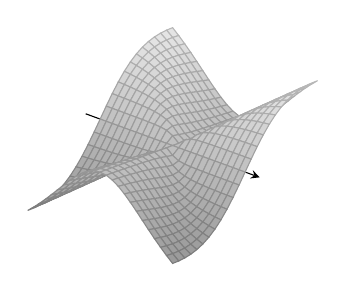
\begin{tikzpicture}[declare function={f(\x,\y)=-\x*(\y)^2/((\x)^2+(\y)^2);}]
  \begin{axis}[view/h=135,width=6cm,axis lines=center,domain=-2:2,domain y=-2:2,colormap={kgray}{gray(0.2cm)=(0.6);gray(1cm)=(0.9);},xtick={\empty},ytick={\empty},ztick={\empty},enlargelimits=true]
%\addplot3[contour gnuplot={output point meta=rawz,number=20,labels=false,},samples=41,z filter/.code=\def\pgfmathresult{-1.6},]{f(x,y)};
 \addplot3[surf,samples=25]{f(x,y)};
%\addplot3[contour gnuplot={draw color = red,levels={0.1,0.2,0.4}}]{f(x,y)};
\end{axis}
\end{tikzpicture}
\caption{}
\label{شکل_سوال_کثیرالمتغیر_ب}
\end{minipage}\hfill
\begin{minipage}{0.3\textwidth}
\centering
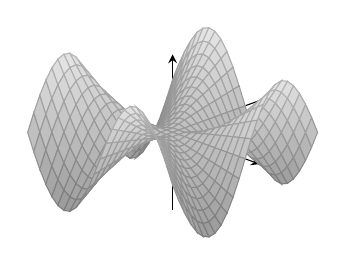
\begin{tikzpicture}[declare function={f(\x,\y)=\x*\y*((\x)^2-(\y)^2)/((\x)^2+(\y)^2);}]
  \begin{axis}[view/h=135,width=6cm,axis lines=center,domain=-2:2,domain y=-2:2,colormap={kgray}{gray(0.2cm)=(0.6);gray(1cm)=(0.9);},xtick={\empty},ytick={\empty},ztick={\empty},enlargelimits=true]
%\addplot3[contour gnuplot={output point meta=rawz,number=20,labels=false,},samples=41,z filter/.code=\def\pgfmathresult{-1.6},]{f(x,y)};
 \addplot3[surf,samples=25]{f(x,y)};
%\addplot3[contour gnuplot={draw color = red,levels={0.1,0.2,0.4}}]{f(x,y)};
\end{axis}
\end{tikzpicture}
\caption{}
\label{شکل_سوال_کثیرالمتغیر_ہ}
\end{minipage}\hfill
\begin{minipage}{0.3\textwidth}
\centering
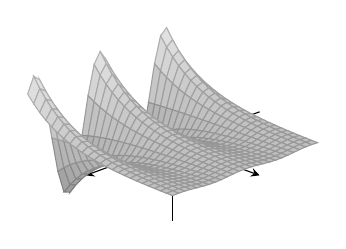
\begin{tikzpicture}[declare function={f(\x,\y)=e^(-\y)*cos(deg(\x));}]
  \begin{axis}[view/h=135,width=6cm,axis lines=center,domain=-7:7,domain y=-2:2,colormap={kgray}{gray(0.2cm)=(0.6);gray(1cm)=(0.9);},xtick={\empty},ytick={\empty},ztick={\empty},enlargelimits=true]
%\addplot3[contour gnuplot={output point meta=rawz,number=20,labels=false,},samples=41,z filter/.code=\def\pgfmathresult{-1.6},]{f(x,y)};
 \addplot3[surf,samples=25]{f(x,y)};
%\addplot3[contour gnuplot={draw color = red,levels={0.1,0.2,0.4}}]{f(x,y)};
\end{axis}
\end{tikzpicture}
\caption{}
\label{شکل_سوال_کثیرالمتغیر_د}
\end{minipage}
\begin{minipage}{0.3\textwidth}
\centering
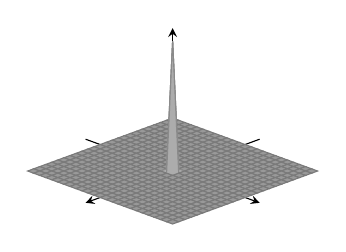
\begin{tikzpicture}[declare function={f(\x,\y)=1/(4*(\x)^2+(\y)^2);}]
  \begin{axis}[view/h=135,width=6cm,axis lines=center,domain=-2:2,domain y=-2:2,colormap={kgray}{gray(0.2cm)=(0.6);gray(1cm)=(0.9);},xtick={\empty},ytick={\empty},ztick={\empty},enlargelimits=true]
%\addplot3[contour gnuplot={output point meta=rawz,number=20,labels=false,},samples=41,z filter/.code=\def\pgfmathresult{-1.6},]{f(x,y)};
 \addplot3[surf,samples=25]{f(x,y)};
%\addplot3[contour gnuplot={draw color = red,levels={0.1,0.2,0.4}}]{f(x,y)};
\end{axis}
\end{tikzpicture}
\caption{}
\label{شکل_سوال_کثیرالمتغیر_ج}
\end{minipage}\hfill
\begin{minipage}{0.3\textwidth}
\centering
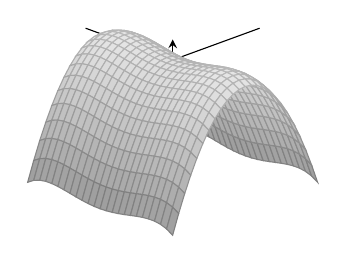
\begin{tikzpicture}[declare function={f(\x,\y)=(\y)^2-(\y)^4-(\x)^2;}]
  \begin{axis}[view/h=135,width=6cm,axis lines=center,domain=-2:2,domain y=-1:1,colormap={kgray}{gray(0.2cm)=(0.6);gray(1cm)=(0.9);},xtick={\empty},ytick={\empty},ztick={\empty},enlargelimits=true]
%\addplot3[contour gnuplot={output point meta=rawz,number=20,labels=false,},samples=41,z filter/.code=\def\pgfmathresult{-1.6},]{f(x,y)};
 \addplot3[surf,samples=25]{f(x,y)};
%\addplot3[contour gnuplot={draw color = red,levels={0.1,0.2,0.4}}]{f(x,y)};
\end{axis}
\end{tikzpicture}
\caption{}
\label{شکل_سوال_کثیرالمتغیر_و}
\end{minipage}\hfill
\begin{minipage}{0.3\textwidth}
\centering
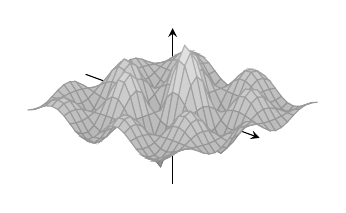
\begin{tikzpicture}[declare function={f(\x,\y)=cos(deg(\x))*sin(deg(\y))*e^(-1/4*sqrt((\x)^2+(\y)^2));}]
  \begin{axis}[view/h=135,width=6cm,axis lines=center,domain=-7:7,domain y=-7:7,colormap={kgray}{gray(0.2cm)=(0.6);gray(1cm)=(0.9);},xtick={\empty},ytick={\empty},ztick={\empty},enlargelimits=true]
%\addplot3[contour gnuplot={output point meta=rawz,number=20,labels=false,},samples=41,z filter/.code=\def\pgfmathresult{-1.6},]{f(x,y)};
 \addplot3[surf,samples=25]{f(x,y)};
%\addplot3[contour gnuplot={draw color = red,levels={0.1,0.2,0.4}}]{f(x,y)};
\end{axis}
\end{tikzpicture}
\caption{}
\label{شکل_سوال_کثیرالمتغیر_الف}
\end{minipage}
\end{figure}

%=====================
\موٹا{دو متغیرات کے تفاعل کی پہچان}\\
سوال \حوالہ{سوال_کثیرالمتغیر_ہم_قد_منحنیات_الف} تا سوال \حوالہ{سوال_کثیرالمتغیر_ہم_قد_منحنیات_ب} میں تفاعل کی قیمتوں کو دو طرح دکھائیں۔ (ا)  سطح \عددی{z=f(x,y)} کو ترسیم کرتے ہوئے اور (ب) تفاعل کے دائرہ کار میں منتخب ہم قد منحنیات ترسیم کرتے ہوئے۔ ہر ایک  ہم قد  منحنی  کی نشاندہی  تفاعل کی قیمت سے کریں۔  

\ابتدا{سوال}\شناخت{سوال_کثیرالمتغیر_ہم_قد_منحنیات_الف}
$f(x,y)=y^2$
\ابتدا{جواب}
\wf{\unexpanded{
\begin{minipage}{0.45\textwidth}
\centering
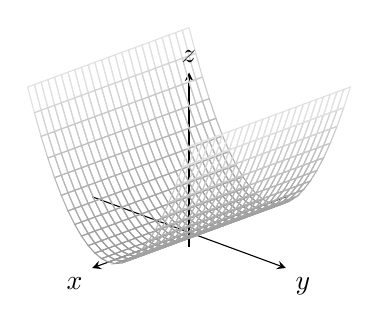
\begin{tikzpicture}[declare function={f(\x,\y)=(\y)^2;}]
  \begin{axis}[view/h=135,small,axis lines=center,domain=-1:1,domain y=-1:1,colormap={kgray}{gray(0.2cm)=(0.6);gray(1cm)=(0.9);},xtick={\empty},ytick={\empty},ztick={\empty},enlargelimits=true,xlabel={$x$},ylabel={$y$},zlabel={$z$},xlabel style={anchor=north east},ylabel style={anchor=north west},zlabel style={anchor=south}]
%\addplot3[, contour gnuplot={output point meta=rawz,number=4,labels=false,},samples=41,z filter/.code=\def\pgfmathresult{-1.6},]{f(x,y)};
 \addplot3[mesh,samples=25]{f(x,y)};
%\addplot3[, contour gnuplot={draw color = red,levels={0.1,0.2,0.4}}]{f(x,y)};
\end{axis}
\end{tikzpicture}
\end{minipage}\hfill
\begin{minipage}{0.45\textwidth}
\centering
\begin{tikzpicture}[declare function={f(\x,\y)=(\y)^2;}]
  \begin{axis}[view/h=135,small,axis lines=center,domain=-1:1,domain y=-1:1,colormap={kgray}{gray(0.2cm)=(0.6);gray(1cm)=(0.9);},xtick={\empty},ytick={\empty},ztick={\empty},enlargelimits=true,hide z axis,,xlabel={$x$},ylabel={$y$},zlabel={$z$},xlabel style={anchor=north east},ylabel style={anchor=north west},zlabel style={anchor=south},colormap={kdark}{gray(0.2cm)=(0.2);gray(1cm)=(0.2);}]
\addplot3[, contour gnuplot={output point meta=rawz,number=4,labels=true,},samples=41,z filter/.code=\def\pgfmathresult{0},]{f(x,y)};
 %\addplot3[mesh,samples=25]{f(x,y)};
%\addplot3[, contour gnuplot={draw color = red,levels={0.1,0.2,0.4}}]{f(x,y)};
\end{axis}
\end{tikzpicture}
\end{minipage}
}}
\انتہا{جواب}
\انتہا{سوال}
%===================
\ابتدا{سوال}
$f(x,y)=4-y^2$
\انتہا{سوال}
%===================
\ابتدا{سوال}
$f(x,y)=x^2+y^2$
\ابتدا{جواب}
\wf{\unexpanded{
\begin{minipage}{0.45\textwidth}
\centering
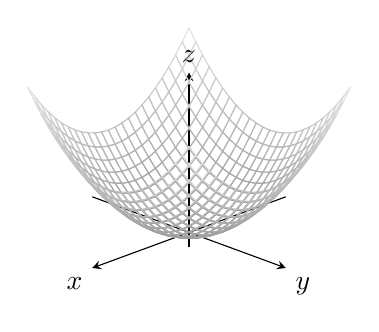
\begin{tikzpicture}[declare function={f(\x,\y)=(\x)^2+(\y)^2;}]
  \begin{axis}[view/h=135,small,axis lines=center,domain=-1:1,domain y=-1:1,colormap={kgray}{gray(0.2cm)=(0.6);gray(1cm)=(0.9);},xtick={\empty},ytick={\empty},ztick={\empty},enlargelimits=true,xlabel={$x$},ylabel={$y$},zlabel={$z$},xlabel style={anchor=north east},ylabel style={anchor=north west},zlabel style={anchor=south}]
%\addplot3[, contour gnuplot={output point meta=rawz,number=4,labels=false,},samples=41,z filter/.code=\def\pgfmathresult{-1.6},]{f(x,y)};
 \addplot3[mesh,samples=25]{f(x,y)};
%\addplot3[, contour gnuplot={draw color = red,levels={0.1,0.2,0.4}}]{f(x,y)};
\end{axis}
\end{tikzpicture}
\end{minipage}\hfill
\begin{minipage}{0.45\textwidth}
\centering
\begin{tikzpicture}[declare function={f(\x,\y)=(\x)^2+(\y)^2;}]
  \begin{axis}[view/h=135,small,axis lines=center,domain=-1:1,domain y=-1:1,colormap={kgray}{gray(0.2cm)=(0.6);gray(1cm)=(0.9);},xtick={\empty},ytick={\empty},ztick={\empty},enlargelimits=true,hide z axis,xlabel={$x$},ylabel={$y$},zlabel={$z$},xlabel style={anchor=north east},ylabel style={anchor=north west},zlabel style={anchor=south},colormap={kdark}{gray(0.2cm)=(0.2);gray(1cm)=(0.2);}]
\addplot3[, contour gnuplot={output point meta=rawz,number=4,labels=true,},samples=41,z filter/.code=\def\pgfmathresult{0},]{f(x,y)};
 %\addplot3[mesh,samples=25]{f(x,y)};
%\addplot3[, contour gnuplot={draw color = red,levels={0.1,0.2,0.4}}]{f(x,y)};
\end{axis}
\end{tikzpicture}
\end{minipage}
}}
\انتہا{جواب}
\انتہا{سوال}
%===================
\ابتدا{سوال}
$f(x,y)=\sqrt{x^2+y^2}$
\انتہا{سوال}
%===================
\ابتدا{سوال}
$f(x,y)=-(x^2+y^2)$
\ابتدا{جواب}
\wf{\unexpanded{
\begin{minipage}{0.45\textwidth}
\centering
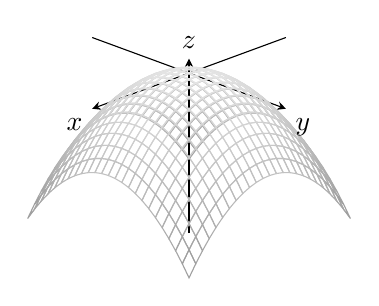
\begin{tikzpicture}[declare function={f(\x,\y)=-(\x)^2-(\y)^2;}]
  \begin{axis}[view/h=135,small,axis lines=center,domain=-1:1,domain y=-1:1,colormap={kgray}{gray(0.2cm)=(0.6);gray(1cm)=(0.9);},xtick={\empty},ytick={\empty},ztick={\empty},enlargelimits=true,xlabel={$x$},ylabel={$y$},zlabel={$z$},xlabel style={anchor=north east},ylabel style={anchor=north west},zlabel style={anchor=south}]
%\addplot3[, contour gnuplot={output point meta=rawz,number=4,labels=false,},samples=41,z filter/.code=\def\pgfmathresult{-1.6},]{f(x,y)};
 \addplot3[mesh,samples=25]{f(x,y)};
%\addplot3[, contour gnuplot={draw color = red,levels={0.1,0.2,0.4}}]{f(x,y)};
\end{axis}
\end{tikzpicture}
\end{minipage}\hfill
\begin{minipage}{0.45\textwidth}
\centering
\begin{tikzpicture}[declare function={f(\x,\y)=-(\x)^2-(\y)^2;}]
  \begin{axis}[view/h=135,width=6cm,axis lines=center,domain=-1:1,domain y=-1:1,colormap={kgray}{gray(0.2cm)=(0.6);gray(1cm)=(0.9);},xtick={\empty},ytick={\empty},ztick={\empty},enlargelimits=true,hide z axis,xlabel={$x$},ylabel={$y$},zlabel={$z$},xlabel style={anchor=north east},ylabel style={anchor=north west},zlabel style={anchor=south},colormap={kdark}{gray(0.2cm)=(0.2);gray(1cm)=(0.2);}]
\addplot3[, contour gnuplot={output point meta=rawz,number=4,labels=true,},samples=41,z filter/.code=\def\pgfmathresult{0},]{f(x,y)};
 %\addplot3[mesh,samples=25]{f(x,y)};
%\addplot3[, contour gnuplot={draw color = red,levels={0.1,0.2,0.4}}]{f(x,y)};
\end{axis}
\end{tikzpicture}
\end{minipage}
}}
\انتہا{جواب}
\انتہا{سوال}
%===================
\ابتدا{سوال}
$f(x,y)=4-x^2-y^2$
\انتہا{سوال}
%===================
\ابتدا{سوال}
$f(x,y)=4x^2+y^2$
\ابتدا{جواب}
\wf{\unexpanded{
\begin{minipage}{0.45\textwidth}
\centering
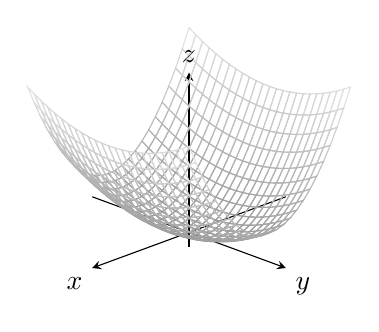
\begin{tikzpicture}[declare function={f(\x,\y)=4*(\x)^2+(\y)^2;}]
  \begin{axis}[view/h=135,small,axis lines=center,domain=-1:1,domain y=-1:1,colormap={kgray}{gray(0.2cm)=(0.6);gray(1cm)=(0.9);},xtick={\empty},ytick={\empty},ztick={\empty},enlargelimits=true,xlabel={$x$},ylabel={$y$},zlabel={$z$},xlabel style={anchor=north east},ylabel style={anchor=north west},zlabel style={anchor=south}]
%\addplot3[, contour gnuplot={output point meta=rawz,number=4,labels=false,},samples=41,z filter/.code=\def\pgfmathresult{-1.6},]{f(x,y)};
 \addplot3[mesh,samples=25]{f(x,y)};
%\addplot3[, contour gnuplot={draw color = red,levels={0.1,0.2,0.4}}]{f(x,y)};
\end{axis}
\end{tikzpicture}
\end{minipage}\hfill
\begin{minipage}{0.45\textwidth}
\centering
\begin{tikzpicture}[declare function={f(\x,\y)=4*(\x)^2+(\y)^2;}]
  \begin{axis}[view/h=135,small,axis lines=center,domain=-1:1,domain y=-1:1,colormap={kgray}{gray(0.2cm)=(0.6);gray(1cm)=(0.9);},xtick={\empty},ytick={\empty},ztick={\empty},enlargelimits=true,hide z axis,xlabel={$x$},ylabel={$y$},zlabel={$z$},xlabel style={anchor=north east},ylabel style={anchor=north west},zlabel style={anchor=south},colormap={kdark}{gray(0.2cm)=(0.2);gray(1cm)=(0.2);}]
\addplot3[, contour gnuplot={output point meta=rawz,number=4,labels=true,},samples=41,z filter/.code=\def\pgfmathresult{0},]{f(x,y)};
 %\addplot3[mesh,samples=25]{f(x,y)};
%\addplot3[, contour gnuplot={draw color = red,levels={0.1,0.2,0.4}}]{f(x,y)};
\end{axis}
\end{tikzpicture}
\end{minipage}
}}
\انتہا{جواب}
\انتہا{سوال}
%===================
\ابتدا{سوال}
$f(x,y)=4x^2+y^2+1$
\انتہا{سوال}
%===================
\ابتدا{سوال}
$f(x,y)=1-\abs{y}$
\ابتدا{جواب}
\wf{\unexpanded{
\begin{minipage}{0.45\textwidth}
\centering
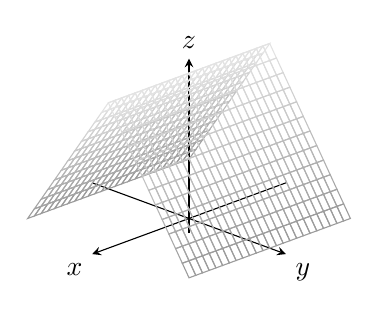
\begin{tikzpicture}[declare function={f(\x,\y)=1-abs(\y);}]
  \begin{axis}[view/h=135,small,axis lines=center,domain=-1:1,domain y=-1:1,colormap={kgray}{gray(0.2cm)=(0.6);gray(1cm)=(0.9);},xtick={\empty},ytick={\empty},ztick={\empty},enlargelimits=true,xlabel={$x$},ylabel={$y$},zlabel={$z$},xlabel style={anchor=north east},ylabel style={anchor=north west},zlabel style={anchor=south}]
%\addplot3[, contour gnuplot={output point meta=rawz,number=4,labels=false,},samples=41,z filter/.code=\def\pgfmathresult{-1.6},]{f(x,y)};
 \addplot3[mesh,samples=25]{f(x,y)};
%\addplot3[, contour gnuplot={draw color = red,levels={0.1,0.2,0.4}}]{f(x,y)};
\end{axis}
\end{tikzpicture}
\end{minipage}\hfill
\begin{minipage}{0.45\textwidth}
\centering
\begin{tikzpicture}[declare function={f(\x,\y)=1-abs(\y);}]
  \begin{axis}[view/h=135,small,axis lines=center,domain=-1:1,domain y=-1:1,colormap={kgray}{gray(0.2cm)=(0.6);gray(1cm)=(0.9);},xtick={\empty},ytick={\empty},ztick={\empty},enlargelimits=true,hide z axis,xlabel={$x$},ylabel={$y$},zlabel={$z$},xlabel style={anchor=north east},ylabel style={anchor=north west},zlabel style={anchor=south},colormap={kdark}{gray(0.2cm)=(0.2);gray(1cm)=(0.2);}]
\addplot3[, contour gnuplot={output point meta=rawz,number=4,labels=true,},samples=41,z filter/.code=\def\pgfmathresult{0},]{f(x,y)};
 %\addplot3[mesh,samples=25]{f(x,y)};
%\addplot3[, contour gnuplot={draw color = red,levels={0.1,0.2,0.4}}]{f(x,y)};
\end{axis}
\end{tikzpicture}
\end{minipage}
}}
\انتہا{جواب}
\انتہا{سوال}
%===================
\ابتدا{سوال}\شناخت{سوال_کثیرالمتغیر_ہم_قد_منحنیات_ب}
$f(x,y)=1-\abs{x}-\abs{y}$
\انتہا{سوال}
%===================

\موٹا{ہم قد سطحیں}\\
سوال \حوالہ{سوال_کثیر_المتغیر_ہم_قد_سطح_الف} تا سوال \حوالہ{سوال_کثیر_المتغیر_ہم_قد_سطح_ب} میں تفاعل کا  ایک علامتی  ہم قد سطح  کا خاکہ بنائیں۔

\ابتدا{سوال}\شناخت{سوال_کثیر_المتغیر_ہم_قد_سطح_الف}
$f(x,y,z)=x^2+y^2+z^2$
\ابتدا{جواب}
\wf{\unexpanded{
\begin{center}
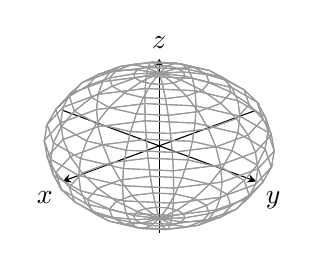
\begin{tikzpicture}[declare function={fx(\x,\y)=sin(\x)*cos(\y);fy(\x,\y)=sin(\x)*sin(\y);fz(\x,\y)=cos(\x);}]
  \begin{axis}[view/h=135,small,axis lines=center,domain=0:180,domain y=0:360,colormap={kgray}{gray(0.2cm)=(0.6);gray(1cm)=(0.6);},xtick={\empty},ytick={\empty},ztick={\empty},enlargelimits=true,xlabel={$x$},ylabel={$y$},zlabel={$z$},xlabel style={anchor=north east},ylabel style={anchor=north west},zlabel style={anchor=south}]
%\addplot3[, contour gnuplot={output point meta=rawz,number=4,labels=false,},samples=41,z filter/.code=\def\pgfmathresult{0},]{f(x,y)};
 \addplot3[mesh,samples=15]({fx(x,y)},{fy(x,y)},{fz(x,y)});
%\addplot3[, contour gnuplot={draw color = red,levels={0.1,0.2,0.4}}]({fx(x,y)},{fy(x,y)},{fz(x,y)});
\end{axis}
\end{tikzpicture}
\end{center}
$f(x,y,z)=x^2+y^2+z^2=1$
}}
\انتہا{جواب}
\انتہا{سوال}
%==================
\ابتدا{سوال}
$f(x,y,z)=\ln(x^2+y^2+z^2)$
\انتہا{سوال}
%================
\ابتدا{سوال}
$f(x,y,z)=x+z$
\ابتدا{جواب}
\wf{\unexpanded{
\begin{center}
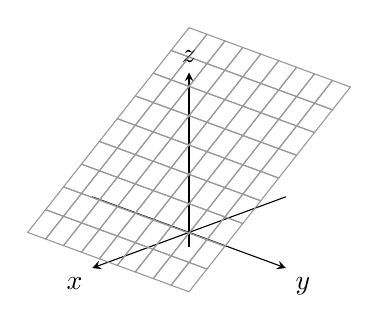
\begin{tikzpicture}[declare function={f(\x,\y)=1-\x;}]
  \begin{axis}[view/h=135,small,axis lines=center,domain=-1:1,domain y=-1:1,colormap={kgray}{gray(0.2cm)=(0.6);gray(1cm)=(0.6);},xtick={\empty},ytick={\empty},ztick={\empty},enlargelimits=true,xlabel={$x$},ylabel={$y$},zlabel={$z$},xlabel style={anchor=north east},ylabel style={anchor=north west},zlabel style={anchor=south}]
%\addplot3[, contour gnuplot={output point meta=rawz,number=4,labels=false,},samples=41,z filter/.code=\def\pgfmathresult{0},]{f(x,y)};
 \addplot3[mesh,samples=10]{f(x,y)};
%\addplot3[, contour gnuplot={draw color = red,levels={0.1,0.2,0.4}}]{f(x,y)};
\end{axis}
\end{tikzpicture}
\end{center}
$f(x,y,z)=x+z=1$
}}
\انتہا{جواب}
\انتہا{سوال}
%================
\ابتدا{سوال}
$f(x,y,z)=z$
\انتہا{سوال}
%================
\ابتدا{سوال}
$f(x,y,z)=x^2+y^2$
\ابتدا{جواب}
\wf{\unexpanded{
\begin{center}
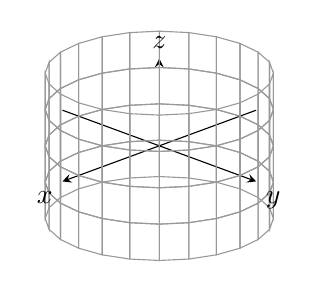
\begin{tikzpicture}[declare function={fx(\x,\y)=cos(\x);fy(\x,\y)=sin(\x);fz(\x,\y)=\y;}]
  \begin{axis}[view/h=135,small,axis lines=center,domain=0:360,domain y=-1:1,colormap={kgray}{gray(0.2cm)=(0.6);gray(1cm)=(0.6);},xtick={\empty},ytick={\empty},ztick={\empty},enlargelimits=true,xlabel={$x$},ylabel={$y$},zlabel={$z$},xlabel style={anchor=north east},ylabel style={anchor=north west},zlabel style={anchor=south}]
%\addplot3[, contour gnuplot={output point meta=rawz,number=4,labels=false,},samples=41,z filter/.code=\def\pgfmathresult{0},]{f(x,y)};
 \addplot3[smooth,mesh,samples=25,samples y=5]({fx(x,y)},{fy(x,y)},{fz(x,y)});
%\addplot3[, contour gnuplot={draw color = red,levels={0.1,0.2,0.4}}]({fx(x,y)},{fy(x,y)},{fz(x,y)});
\end{axis}
\end{tikzpicture}
\end{center}
$f(x,y,z)=x^2+y^2=1$
}}
\انتہا{جواب}
\انتہا{سوال}
%================
\ابتدا{سوال}
$f(x,y,z)=y^2+z^2$
\انتہا{سوال}
%================
\ابتدا{سوال}
$f(x,y,z)=z-x^2-y^2$
\ابتدا{جواب}
\wf{\unexpanded{
\begin{center}
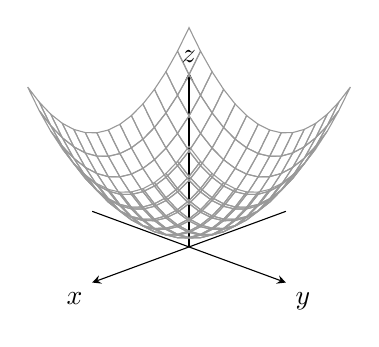
\begin{tikzpicture}[declare function={f(\x,\y)=1+(\x)^2+(\y)^2;}]
  \begin{axis}[view/h=135,small,axis lines=center,domain=-1:1,domain y=-1:1,colormap={kgray}{gray(0.2cm)=(0.6);gray(1cm)=(0.6);},xtick={\empty},ytick={\empty},ztick={\empty},enlargelimits=true,xlabel={$x$},ylabel={$y$},zlabel={$z$},xlabel style={anchor=north east},ylabel style={anchor=north west},zlabel style={anchor=south}]
%\addplot3[, contour gnuplot={output point meta=rawz,number=4,labels=false,},samples=41,z filter/.code=\def\pgfmathresult{0},]{f(x,y)};
 \addplot3[mesh,samples=15]{f(x,y)};
%\addplot3[, contour gnuplot={draw color = red,levels={0.1,0.2,0.4}}]{f(x,y)};
\end{axis}
\end{tikzpicture}
\end{center}
$f(x,y,z)=z-x^2-y^2=1$\\
یعنی
$z=x^2+y^2+1$
}}
\انتہا{جواب}
\انتہا{سوال}
%================
\ابتدا{سوال}\شناخت{سوال_کثیر_المتغیر_ہم_قد_سطح_ب}
$f(x,y,z)=\tfrac{x^2}{25}+\tfrac{y^2}{16}+\tfrac{z^2}{9}$
\انتہا{سوال}
%================
\موٹا{ہم قد منحنی کی  تلاش}\\
سوال \حوالہ{سوال_کثیر_المتغیر_ہم_قد_منحنی_تلاش_الف} تا سوال \حوالہ{سوال_کثیر_المتغیر_ہم_قد_منحنی_تلاش_ب} میں  تفاعل \عددی{f(x,y)} کی اس  ہم قد منحنی کی مساوات تلاش کریں جو  دیے گئے نقطہ سے گزرتی  ہو۔

\ابتدا{سوال}\شناخت{سوال_کثیر_المتغیر_ہم_قد_منحنی_تلاش_الف}
$f(x,y)=16-x^2-y^2,\quad (2\sqrt{2},\sqrt{2})$
\ابتدا{جواب}
\wf{\unexpanded{
$x^2+y^2=10$
}}
\انتہا{جواب}
\انتہا{سوال}
%================
\ابتدا{سوال}
$f(x,y)=\sqrt{x^2-1},\quad (1,0)$
\انتہا{سوال}
%================
\ابتدا{سوال}
$f(x,y)=\int\limits_x^y\frac{\dif t}{1+t^2},\quad (-\sqrt{2},\sqrt{2})$
\ابتدا{جواب}
\wf{\unexpanded{
$\tan^{-1}y-\tan^{-1}x=2\tan^{-1}\sqrt{2}$
}}
\انتہا{جواب}
\انتہا{سوال}
%================
\ابتدا{سوال}\شناخت{سوال_کثیر_المتغیر_ہم_قد_منحنی_تلاش_ب}
$f(x,y)=\sum\limits_{n=0}^{\infty}\big(\frac{x}{y}\big)^n,\quad (1,2)$
\انتہا{سوال}
%================
\موٹا{ہم قد سطح کی تلاش}\\
سوال \حوالہ{سوال_کثیر_المتغیر_ہم_قد_سطح_تلاش_الف} تا سوال \حوالہ{سوال_کثیر_المتغیر_ہم_قد_سطح_تلاش_ب} میں دیے گئے نقطہ سے گزرتی ہم قد سطح کی مساوات تلاش کریں۔

\ابتدا{سوال}\شناخت{سوال_کثیر_المتغیر_ہم_قد_سطح_تلاش_الف}
$f(x,y,z)=\sqrt{x-y}-\ln z,\quad (3,-1,1)$
\ابتدا{جواب}
\wf{\unexpanded{
$\sqrt{x-y}-\ln z=2$
}}
\انتہا{جواب}
\انتہا{سوال}
%=================
\ابتدا{سوال}
$f(x,y,z)=\ln(x^2+y+z^2),\quad (-1,2,1)$
\انتہا{سوال}
%==================
\ابتدا{سوال}
$g(x,y,z)=\sum\limits_{n=0}^{\infty}\frac{(x+y)^n}{n!z^n},\quad (\ln 2,\ln 4,3)$
\ابتدا{جواب}
\wf{\unexpanded{
$\tfrac{x+y}{z}=\ln 2$
}}
\انتہا{جواب}
\انتہا{سوال}
%==================
\ابتدا{سوال}\شناخت{سوال_کثیر_المتغیر_ہم_قد_سطح_تلاش_ب}
$g(x,y,z)=\int\limits_x^y\frac{\dif \theta}{\sqrt{1-\theta^2}}+\int\limits_{\sqrt{2}}^{z}\frac{\dif t}{t\sqrt{t^2-1}},\quad (0,\tfrac{1}{2},2)$
\انتہا{سوال}
%==================

\موٹا{نظریہ اور مثالیں}\\
\ابتدا{سوال}\ترچھا{فضا میں ایک لکیر پر تفاعل کی زیادہ سے زیادہ قیمت۔}\\
کیا لکیر \عددی{x=20-t,\,y=t,\,z=20} پر تفاعل \عددی{f(x,y,z)=xyz} کی  زیادہ سے زیادہ قیمت پائی جاتی ہے؟ اگر  ہو، تب اس کی قیمت کتنی ہو گی؟ اپنے جواب کی وجہ پیش کریں۔ (اشارہ:اس لکیر پر \عددی{w=(f,y,z)} متغیر \عددی{t} کا قابل تفرق تفاعل ہے۔)
\ابتدا{جواب}
\wf{\unexpanded{
جی ہاں، \عددی{2000}
}}
\انتہا{جواب}
\انتہا{سوال}
%==============
\ابتدا{سوال}\ترچھا{فضا میں ایک لکیر پر تفاعل کی کم سے کم  قیمت۔}\\
کیا لکیر \عددی{x=t-1,\,y=t-2,\,z=t+7} پر تفاعل \عددی{f(x,y,z)=xy-z} کی کم سے کم  قیمت پائی جاتی ہے؟ اگر  ہو، تب اس کی قیمت کتنی ہو گی؟ اپنے جواب کی وجہ پیش کریں۔ (اشارہ:اس لکیر پر \عددی{w=(f,y,z)} متغیر \عددی{t} کا قابل تفرق تفاعل ہے۔)
\انتہا{سوال}
%=================
\ابتدا{سوال}\ترچھا{جہاز کا صوتی دھماکا}\\
ایک جہاز کے نیچے زمین پر اس خطہ کی چوڑائی \عددی{w}  جہاں  جہاز کا   صوتی دھماکا   انسان  برائے راست (جو   فضا میں ہوا کی مختلف  سطحوں سے منعکس نہ ہو)  سن سکتا ہو  ، درج ذیل کا  تفاعل ہو گا۔
\begin{itemize}
\item
\عددی{T} زمین پر ہوا کی  درجہ حرارت (کیلون) 
\item
\عددی{h} جہاز کی بلندی (کلو میٹر)
\item
\عددی{d}  درجہ حرارت کی انتصابی  شرح تبدیلی (کیلون فی کلومیٹر)
\end{itemize}
اس چوڑائی کا  کلیہ درج ذیل ہے۔
\begin{align*}
w=4\sqrt{\tfrac{Th}{d}}
\end{align*}
یہ جہاز \عددی{\SI{16.8}{\kilo\meter}} کی بلندی پر پرواز کرتا ہوا  بحیرہ عرب  سے کراچی  شہر    پہنچ رہا ہے۔ اگر سطحی درجہ حرارت \عددی{\SI{290}{\kelvin}} اور انتصابی شرح حرارت \عددی{\SI{5}{\kelvin\per\kilo\meter}} ہو تب   جہاز ساحل سے کتنا دور ہو گا جب اس کا صوتی دھماکا سنائی دے۔
\ابتدا{جواب}
\wf{\unexpanded{
$\SI{63}{\kilo\meter}$
}}
\انتہا{جواب}
\انتہا{سوال}
%================
\ابتدا{سوال}
جیسا کہ آپ جانتے ہیں، واحد حقیقی متغیر کے حقیقی قیمت تفاعل کی ترسیم دو محددی فضا کا سلسلہ ہو تا ہے۔ دو غیر تابع حقیقی متغیرات کے حقیقی قیمت تفاعل  کی ترسیم تین محددی فضا کا سلسلہ ہوتا ہے۔    تین غیر تابع حقیقی متغیرات کے حقیقی قیمت تفاعل  کی ترسیم چار  محددی فضا کا سلسلہ ہوتا ہے۔   آپ چار غیر تابع متغیرات کے تفاعل \عددی{f(x_1,x_2,x_3,x_4)}  کی ترسیم کے بارے میں کیا کہیں گے؟ ۔   آپ \عددی{n}  غیر تابع متغیرات کے تفاعل \عددی{f(x_1,x_2,x_3,\cdots,x_n)}  کی ترسیم کے بارے میں کیا کہیں گے؟
\انتہا{سوال}
%==========
\موٹا{کمپیوٹر کا استعمال۔صریح سطح}\\
کمپیوٹر استعمال کرتے ہوئے سوال \حوالہ{سوال_کثیرالمتغیر_صریح_سطح_الف} تا سوال \حوالہ{سوال_کثیرالمتغیر_صریح_سطح_ب} میں درج ذیل اقدام کریں۔
\begin{enumerate}[a.]
\item
دیے گئے مستطیل پر سطح ترسیم کریں۔
\item
اس مستطیل میں کئی ہم قد منحنیات ترسیم کریں۔
\item
دیے گئے نقطہ سے گزرتی  ہوئی   \عددی{f} کی   ہم قد منحنی ترسیم کریں۔ 
\end{enumerate}

\ابتدا{سوال}\شناخت{سوال_کثیرالمتغیر_صریح_سطح_الف}
$f(x,y)=x\sin\tfrac{y}{2}+y\sin 2x,\quad 0\le x\le 5\pi,\quad 0\le y\le 5\pi$
\انتہا{سوال}
%=================
\ابتدا{سوال}
$f(x,y)=(\sin x)(\cos x)e^{\sqrt{x^2+y^2}/8},\quad 0\le x\le 5\pi,\quad 0\le y\le 5\pi$
\انتہا{سوال}
%==================
\ابتدا{سوال}
$f(x,y)=\sin(x+2\cos y),\quad -2\pi\le x\le 2\pi,\quad -2\pi\le y\le 2\pi$
\انتہا{سوال}
%==================
\ابتدا{سوال}\شناخت{سوال_کثیرالمتغیر_صریح_سطح_ب}
$f(x,y)=e^{(x^{0.1}-y)}\sin (x^2+y^2),\quad 0\le x\le 2\pi,\quad -2\pi\le y\le \pi$
\انتہا{سوال}
%==================
\موٹا{کمپیوٹر کا استعمال۔خفی  سطح}\\
سوال \حوالہ{سوال_کثیرالمتغیر_ہم_قد_سطحیں_ترسیم_الف} تا سوال \حوالہ{سوال_کثیرالمتغیر_ہم_قد_سطحیں_ترسیم_ب} میں کمپیوٹر استعمال کرتے ہوئے ہم قد سطحیں  ترسیم کریں۔

\ابتدا{سوال}\شناخت{سوال_کثیرالمتغیر_ہم_قد_سطحیں_ترسیم_الف}
$4\ln(x^2+y^2+z^2)=1$
\انتہا{سوال}
%================
\ابتدا{سوال}
$x^2+z^2=1$
\انتہا{سوال}
%=====================
\ابتدا{سوال}
$x+y^2-3z^2=1$
\انتہا{سوال}
%=====================
\ابتدا{سوال}\شناخت{سوال_کثیرالمتغیر_ہم_قد_سطحیں_ترسیم_ب}
$\sin\big(\frac{x}{2}\big)-(\cos y)\sqrt{x^2+z^2}=2$
\انتہا{سوال}
%=====================
\موٹا{کمپیوٹر کا استعمال۔مقدار معلوم   سطح}\\
جیسا آپ کسی مقدار معلوم وقفہ \عددی{I} پر  مستوی میں منحنیات کو مقدار معلوم مساوات \عددی{x=f(t),\,y=g(t)} کی    روپ میں لکھتے ہیں، آپ بعض اوقات کسی مقدار معلوم مستطیل \عددی{a\le u\le b,\, c\le v\le d}وقفہ  پر  فضا میں سطحوں کو    مقدار معلوم تین مساوات \عددی{x=f(u,v),\,y=g(u,v),\,z=h(u,v)}  کی روپ میں لکھ سکتے ہیں۔کمپیوٹر اس قسم کی مقدار معلوم مساواتوں سے سطح  ترسیم کر سکتا ہے۔سوال \حوالہ{سوال_کثیرالمتغیر_مقدار_معلوم_الف} تا سوال \حوالہ{سوال_کثیرالمتغیر_مقدار_معلوم_ب} میں کمپیوٹر کی مدد سے سطحیں ترسیم کریں۔ساتھ ہی \عددی{xy} مستوی میں چند ہم قد منحنیات ترسیم کریں۔

\ابتدا{سوال}\شناخت{سوال_کثیرالمتغیر_مقدار_معلوم_الف}
$x=u\cos v,\quad y=u\sin v,\quad z=u,\quad 0\le u\le 2,\quad 0\le v\le 2\pi$
\انتہا{سوال}
%===================
\ابتدا{سوال}
$x=u\cos v,\quad y=u\sin v,\quad z=v,\quad 0\le u\le 2,\quad 0\le v\le 2\pi$
\انتہا{سوال}
%===================
\ابتدا{سوال}
$x=(2+\cos u)\cos v,\,y=(2+\cos u)\sin v,\, z=\sin u,$\\
$ 0\le u\le 2\pi,\, 0\le v\le 2\pi$
\انتہا{سوال}
%===================
\ابتدا{سوال}\شناخت{سوال_کثیرالمتغیر_مقدار_معلوم_ب}
$x=2\cos u\cos v,\quad y=2\cos u\sin v,\quad z=2\sin u$\\
$0\le u\le 2\pi,\quad 0\le v\le \pi$
\انتہا{سوال}
%======================
\انتہا{سوالات}




\حصہ{حد اور استمرار}
اس حصہ میں کثیر المتغیر تفاعل کی حد اور استمرار پر غور کیا جائے گا۔

\جزوحصہء{حد}
اگر نقطہ \عددی{(x_0,y_0)} کے قریب   تمام نقاط \عددی{(x,y) } کے لئے تفاعل \عددی{f(x,y)}  کی قیمتیں کسی  مقررہ حقیقی عدد \عددی{L} کے  بہت  زیادہ  قریب ہوں تب ہم کہتے ہیں کہ جیسے جیسے \عددی{(x,y)} نقطہ \عددی{(x_0,y_0)} تک  پہنچنے کی کوشش کرتا ہے، تفاعل \عددی{f} کی قیمت \عددی{L} تک پہنچنے کی کوشش کرتی ہے۔ یہ تعریف، واحد متغیر کے تفاعل کی حد کی تعریف کی مانند ہے۔البتہ، دھیان رہے کہ اگر \عددی{(x_0,y_0)} تفاعل \عددی{f}  کے دائرہ کار  کی اندرون میں پایا جاتا ہو تب \عددی{(x,y)} نقطہ \عددی{(x_0,y_0)} تک کسی بھی رخ سے پہنچنے کی کوشش کر سکتا ہے۔جیسا آپ نیچے  دی گئی   مثالوں میں سے چند  میں دیکھیں گے،  قریب پہنچنے کا رخ بعض اوقات مسئلہ کھڑا کر سکتا ہے۔

\ابتدا{تعریف}
اگر ہر عدد \عددی{\epsilon>0} کے لئے ایسا مطابقتی عدد \عددی{\delta>0} پایا جاتا ہو کہ \عددی{f} کے دائرہ کار میں تمام \عددی{(x,y)} کے لئے 
\begin{align}\label{مساوات_کثیرالمتغیر_تعریف_حد_الف}
0<\sqrt{(x-x_0)^2+(y-y_0)^2}<\delta\implies \abs{f(x,y)-L}<\epsilon
\end{align}
ہو ، تب ہم کہتے ہیں کہ \عددی{(x_0,y_0)} تک  \عددی{(x,y)}    پہنچنے سے \عددی{f(x,y)} کی قیمت \اصطلاح{حد}\فرہنگ{حد}\حاشیہب{limit}\فرہنگ{limit} \عددی{L} تک پہنچتی ہے جس کو ہم درج ذیل لکھتے ہیں۔
\begin{align*}
\lim_{(x,y)\to(x_0,y_0)}f(x,y)=L
\end{align*}
\انتہا{تعریف}
%====================

حد کی تعریف میں \عددی{\delta \sigma} کی شرط  اس کی  معادل ہے  کہ، کسی بھی \عددی{\epsilon>0} کے لئے ایسا مطابقتی \عددی{\delta>0} پایا جاتا ہو کہ تمام \عددی{x} کے لئے درج ذیل ہو۔
\begin{align}\label{مساوات_کثیرالمتغیر_تعریف_حد_ب}
0<\abs{x-x_0}<\delta\quad \text{اور}\quad 0<\abs{y-y_0}<\delta\implies \abs{f(x,y)-L}<\epsilon
\end{align}
یوں حد کی قیمت  تلاش کرتے   ہوئے ہم مستوی میں فاصلوں کی صورت یا محدد میں فرق کی صورت میں سوچ سکتے ہیں۔

حد کی تعریف، تفاعل \عددی{f} کے دائرہ کار کی اندرون  کے ساتھ   سرحدی نقاط \عددی{(x_0,y_0)} کے لئے بھی   کارآمد  ہے۔  بس اتنا ضروری ہے کہ نقطہ \عددی{(x,y)} ہر وقت دائرہ کار کے اندر رہے۔

واحد متغیر کے تفاعل کی طرح  درج ذیل دکھائے جا  سکتے ہیں۔
\begin{gather}
\begin{aligned}\label{مساوات_کثیر_المتغیر_قواعد_حد}
\lim_{(x,y)\to(x_0,y_0)}x&=x_0\\
\lim_{(x,y)\to(x_0,y_0)}y&=y_0\\
\lim_{(x,y)\to(x_0,y_0)}k&=k\quad \text{\RL{\عددی{k} کوئی بھی عدد ہو سکتا ہے}}
\end{aligned}
\end{gather}
یہ بھی دکھایا جا سکتا ہے کہ دو تفاعل کے مجموعہ کا حد، ان تفاعل کے انفرادی حد   (اگر دونوں موجود ہوں)کا مجموعہ ہو گا۔اسی طرح   کے نتائج   فرق، حاصل ضرب، حاصل تقسیم، مستقل مضرب اور طاقت کے لئے بھی دکھائے جا سکتے ہیں۔

\ابتدا{مسئلہ}\شناخت{مسئلہ_کثیر_المتغیر_قواعد_حد}\موٹا{دو متغیرات کے تفاعل کی حد کے خواص}\\
اگر 
\begin{align*}
\lim_{(x,y)\to(x_0,y_0)}f(x,y)=L\quad \text{اور}\quad \lim_{(x,y)\to(x_0,y_0)}g(x,y)=M
\end{align*}
ہوں تب درج ذیل قواعد کارآمد  ہوں گے۔
\begin{description}
\item{قاعدہ مجموعہ:}
$\lim[f(x,y)+g(x,y)]=L+M$
\item{قاعدہ فرق:}
$\lim[f(x,y)-g(x,y)]=L-M$
\item{قاعدہ مستقل مضرب:}
$\lim kf(x,y)=kL$
جہاں \عددی{k} کوئی مستقل ہے۔
\item{قاعدہ حاصل تقسیم:}
$\lim\frac{f(x,y)}{g(x,y)}=\frac{L}{M}$
اگر  \عددی{M\ne 0} ہو۔
\item{قاعدہ طاقت:}
$\lim[f(x,y)]^{m/n}=L^{m/n}$
اگر  \عددی{m} اور \عددی{n}ا عداد صحیح   اور \عددی{L^{m/n}} ایک حقیقی عدد ہو۔
\end{description}
تمام حد \عددی{(x,y)\to (x_0,y_0)} کی صورت میں حاصل کیے جائیں گے اور \عددی{L}، \عددی{M} کا حقیقی اعداد ہونا لازمی ہے۔
\انتہا{مسئلہ}
%==========

 مساوات \حوالہ{مساوات_کثیر_المتغیر_قواعد_حد} پر   مسئلہ \حوالہ{مسئلہ_کثیر_المتغیر_قواعد_حد} کے اطلاق سے ہمیں معلوم ہوتا ہے کہ  \عددی{(x,y)\to(x_0,y_0)} کرتے ہوئے  کثیر رکنی اور ناطق تفاعل کی حد     ہم \عددی{(x_0,y_0)} پر  تفاعل کی قیمت   سے حاصل کرتے  ہیں۔ بس اتنا ضروری  ہے کہ  نقطہ \عددی{(x_0,y_0)} پر تفاعل  معین ہو۔

\ابتدا{مثال}
\begin{align*}
\lim_{(x,y)\to(0,1)}\frac{x-xy+3}{x^2y+5xy-y^3}&=\frac{0-(0)(1)+3}{(0)^2(1)+5(0)(1)-(1)^3}=-3\\
\lim_{(x,y)\to(3,-4)}\sqrt{x^2+y^2}&=\sqrt{(3)^2+(-4)^2}=\sqrt{25}=5
\end{align*}
\انتہا{مثال}
%=================
\ابتدا{مثال}
درج ذیل حاصل کریں۔
\begin{align*}
\lim_{(x,y)\to(0,0)}\frac{x^2-xy}{\sqrt{x}-\sqrt{y}}
\end{align*}
حل:\quad
چونکہ \عددی{(x,y)\to(0,0)} پر نسب نما   \عددی{ 0} کو پہنچتا ہے لہٰذا  ہم  قاعدہ حاصل تقسیم (مسئلہ \حوالہ{مسئلہ_کثیر_المتغیر_قواعد_حد})  استعمال نہیں کر سکتے ہیں۔ البتہ نسب نما اور شمار کنندہ کو \عددی{\sqrt{x}+\sqrt{y}} سے ضرب  دے کر ایسا معادل حاصل تقسیم حاصل ہوتا ہے جس کا حد ہم تلاش کر سکتے ہیں:
\begin{align*}
\lim_{(x,y)\to(0,0)}\frac{x^2-xy}{\sqrt{x}-\sqrt{y}}&=\lim_{(x,y)\to(0,0)}\frac{(x^2-xy)(\sqrt{x}+\sqrt{y})}{(\sqrt{x}-\sqrt{y})(\sqrt{x}+\sqrt{y})}\\
&=\lim_{(x,y)\to(0,0)}\frac{x(x-y)(\sqrt{x}+\sqrt{y})}{x-y}&&\text{الجبرا}\\
&=\lim_{(x,y)\to(0,0)}x(\sqrt{x}+\sqrt{y})&&\text{\RL{جزو \عددی{(x-y)} کاٹا گیا}}\\
&=0(\sqrt{0}+\sqrt{0})=0
\end{align*} 
\انتہا{مثال}
%================

\جزوحصہء{استمرار}
واحد متغیر کے تفاعل کی طرح، استمرار کی تعریف  حد کی صورت میں کی جاتی ہے۔

\ابتدا{تعریف}
اگر 
\begin{enumerate}[a.]
\item
\عددی{(x_0,y_0)} پر \عددی{f} معین ہو،
\item
\عددی{\lim_{(x,y)\to(x_0,y_0)}f(x,y)} موجود ہو،
\item
\عددی{\lim_{(x,y)\to(x_0,y_0)}f(x,y)=f(x_0,y_0)} ہو،
\end{enumerate} 
تب تفاعل  \عددی{f}    \اصطلاح{نقطہ \عددی{(x_0,y_0)} پر استمراری}\فرہنگ{استمراری!نقطہ پر}\حاشیہب{continuous}\فرہنگ{continuous!at a point} ہو گا۔ ایک  تفاعل  جو اپنے دائرہ کار کے  ہر نقطہ پر استمراری ہو\اصطلاح{ استمراری}\فرہنگ{استمراری}\حاشیہب{continuous}\فرہنگ{continuous} ہو گا۔
\انتہا{تعریف}
%===============

حد کی تعریف کی طرح،  استمرار کی تعریف بھی \عددی{f} کے دائرہ کار کے تمام اندرونی نقاط کے ساتھ  ساتھ  سرحدی نقاط پر بھی قابل اطلاق  ہوتا ہے بس اتنا ضروری ہے کہ پورے  وقت  نقطہ \عددی{(x,y)}تفاعل کے دائرہ کار میں رہے۔

جیسا آپ  دیکھ سکتے ہیں، مسئلہ \حوالہ{مسئلہ_کثیر_المتغیر_قواعد_حد}    کا ایک نتیجہ  یہ ہے  کہ استمراری تفاعل  کے الجبرائی  جوڑ  ہر اس نقطہ پر استمراری ہوں گے جس پر تمام شامل تفاعل استمراری ہوں۔اس کا مطلب ہے کہ جہاں  تمام   استمراری تفاعل استمراری ہوں وہاں ان  کے مجموعہ، فرق، حاصل ضرب،  مستقل مضرب، حاصل تقسیم اور طاقت استمراری ہوں گے۔   بالخصوص دو متغیرات کی کثیر رکنی اور ناطق تفاعل ان تمام نقطوں پر استمراری ہوں گے جہاں یہ معین ہوں۔

اگر  \عددی{x} اور \عددی{y} کا استمراری تفاعل  \عددی{z=f(x,y)} ہو  جبکہ \عددی{z}  کا استمراری تفاعل \عددی{z=g(z)} ہو، تب  مرکب   \عددی{w=g(f(x,y))}  استمراری ہو گا۔یوں  ہر نقطہ \عددی{(x,y)} پر درج ذیل استمراری ہوں گے۔
\begin{align*}
e^{x-y},\quad \cos\frac{xy}{x^2+1},\quad \ln(1+x^2y^2)
\end{align*}

واحد متغیر کے تفاعل کی طرح، استمراری تفاعل کا  مرکب  بھی استمراری ہو گا،  بس اتنا ضروری ہے کہ وہاں  ہر  تفاعل  استمراری ہو۔

\begin{figure}
\centering
\begin{subfigure}{0.45\textwidth}
\centering
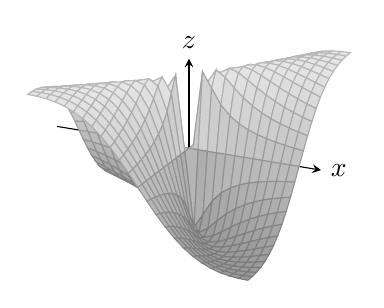
\begin{tikzpicture}[declare function={f(\x,\y)=2*\x*\y/((\x)^2+(\y)^2);}]
  \begin{axis}[small,axis lines=center,colormap={}{gray(0.2cm)=(0.6);gray(1cm)=(0.9);},enlargelimits=true,xlabel={$x$},ylabel={$y$},zlabel={$z$},hide y axis,xlabel style={anchor={west}},zlabel style={anchor=south},xtick={\empty},ytick={\empty},ztick={\empty}]
    \addplot3[surf] { (x==0&&y==0) ?0 : f(x,y) } ;
  \end{axis}
\end{tikzpicture}
\end{subfigure}\hfill
\begin{subfigure}{0.45\textwidth}
\centering
\begin{tikzpicture}[declare function={f(\x,\y)=2*\x*\y/((\x)^2+(\y)^2);}]
  \begin{axis}[small,axis lines=center,colormap={}{gray(0.2cm)=(0.6);gray(1cm)=(0.9);},enlargelimits=true,xlabel={$x$},ylabel={$y$},zlabel={$z$},xlabel style={anchor={west}},ylabel style={anchor=south west},zlabel style={anchor=south},xtick={\empty},ytick={\empty},ztick={\empty},hide z axis]
\addplot3[contour gnuplot={output point meta=rawz,number=5,labels=false,},samples=41,z filter/.code=\def\pgfmathresult{0},]{f(x,y)};
\addplot3[] coordinates {(0,0,0)}coordinate(ka);
  \end{axis}
\draw[fill=white](ka) circle (2pt);
\end{tikzpicture}
\end{subfigure}
\caption{ماسوائے نقطہ \عددی{(0,0)} تفاعل \عددی{f(x,y)} استمراری ہے۔}
\label{شکل_مثال_کثیرالمتغیر_حد_یکتا_ضروری}
\end{figure}

\ابتدا{مثال}\شناخت{مثال_کثیرالمتغیر_حد_یکتا_ضروری}
دکھائیں کہ ماسوائے مبدا   درج ذیل ہر نقطہ پر استمراری ہے (شکل \حوالہ{شکل_مثال_کثیرالمتغیر_حد_یکتا_ضروری})۔
\begin{align*}
f(x,y)=
\begin{cases}
\frac{2xy}{x^2+y^2},&(x,y)\ne (0,0)\\
0,&(x,y)=(0,0)
\end{cases}
\end{align*}
حل:\quad
ہر نقطہ \عددی{(x,y)\ne (0,0)} پر تفاعل کی قیمت \عددی{x} اور \عددی{y}کے  ناطق تفاعل سے حاصل کی جاتی ہے لہٰذا   \عددی{f}   استمراری ہو گا۔

نقطہ \عددی{(0,0)} پر \عددی{f}  کی قیمت معین ہے، لیکن ہم دعویٰ کرتے ہیں کہ \عددی{(x,y)\to(0,0)} کرتے ہوئے اس کا حد غیر موجود ہے۔اس کی وجہ، جیسا ہم دیکھیں گے،   یہ ہے کہ مبدا تک مختلف راہوں سے پہنچتے ہوئے مختلف  نتائج حاصل ہوتے ہیں۔

درج ذیل کی بنا، سوراخ دار لکیر \عددی{y=mx,\, x\ne 0} پر \عددی{m} کی ہر قیمت کے لئے تفاعل \عددی{f} کی ایک مستقل قیمت  ہو گی۔
\begin{align*}
\left. f(x,y)\right\vert_{y=mx}=\left. \frac{2xy}{x^2+y^2}\right\vert_{y=mx}=\frac{2x(mx)}{x^2+(mx)^2}=\frac{2mx^2}{x^2+m^2x^2}=\frac{2m}{1+m^2}
\end{align*}
یوں  اس لکیر  پر جیسے جیسے   \عددی{(x,y)} مبدا تک پہنچتا ہے،  \عددی{f} کی حد اتنی ہو گی:
\begin{align*}
\lim_{\substack{(x,y)\to(0,0)\\ \text{\RL{خط $y=mx$ پر}}}} f(x,y)=\lim_{(x,y)\to(0,0)}\big[\left.f(x,y)\right\vert_{y=mx}\big]=\frac{2m}{1+m^2}
\end{align*}
ہم دیکھتے ہیں کہ حد کی قیمت \عددی{m} پر منحصر ہے۔یوں ایسی کوئی   یکتا قیمت حاصل نہیں ہوتی  جس کو    مبدا تک \عددی{(x,y)} پہنچنے   پر ہم  \عددی{f}  کی حد کہہ سکیں۔ مبدا پر حد غیر موجود ہے لہٰذا مبدا  پر تفاعل غیر استمراری ہو گا۔
\انتہا{مثال}
%=============

دو  (یا دو سے زیادہ)متغیرات کے تفاعل کے حد کے بارے میں ایک اہم نقطہ مثال \حوالہ{مثال_کثیرالمتغیر_حد_یکتا_ضروری} میں  اجاگر ہوا۔ ایک نقطہ پر حد کی موجودگی کے لئے  ضروری ہے کہ اس نقطہ تک  تمام آمد    راہوں  پر  حد  کی قیمت ایک جیسی ہو۔  یوں جب بھی ہم ایک نقطہ  تک  ایسی راہیں  تلاش  کریں جن  پر حد ایک دوسرے سے  مختلف ہوں  تب  اس نقطہ پر تفاعل کا حد غیر موجود ہو گا۔

\ابتدا{پرکھ}\موٹا{حد کی غیر موجودگی کی  دو راہ  پرکھ}\\
اگر \عددی{(x_0,y_0)} تک نقطہ \عددی{(x,y)} ایسی دو مختلف راہوں سے پہنچے جن پر \عددی{f(x,y)} کے حد ایک دوسرے سے مختلف ہوں تب \عددی{\lim\limits_{(x,y)\to(x_0,y_0)}f(x,y)} غیر موجود ہو گا۔
\انتہا{پرکھ}
%===================

\ابتدا{مثال}\شناخت{مثال_کثیرالمتغیر_مبدا_پر_غیر_استمراری_سطح_ب}
دکھائیں کہ \عددی{(0,0)} تک \عددی{(x,y)} پہنچنے سے درج ذیل تفاعل کا کوئی حد حاصل نہیں ہوتا ہے (شکل \حوالہ{شکل_مثال_کثیرالمتغیر_مبدا_پر_غیر_استمراری_سطح_ب})۔
\begin{align*}
f(x,y)=\frac{2x^2y}{x^4+y^2}
\end{align*}
حل:\quad
منحنی \عددی{y=kx^2,\, x\ne 0} پر اس تفاعل کی قیمت ایک مستقل ہے:
\begin{align*}
\left.f(x,y)\right\vert_{y=kx^2}=\left.\frac{2x^2y}{x^4+y^2}\right\vert_{y=kx^2}=\frac{2x^2(kx^2)}{x^4+(kx^2)^2}=\frac{2kx^4}{x^4+k^2x^4}=\frac{2k}{1+k^2}
\end{align*}  
یوں
\begin{align*}
\lim_{\substack{(x,y)\to (0,0)\\ \text{\RL{$y=kx^2$ پر}}}}f(x,y)=\lim_{(x,y)\to(0,0)}\big[\left.f(x,y)\right\vert_{y=kx^2}\big]=\frac{2k}{1+k^2}
\end{align*}
ہو گا  جو   آمد راہ  پر منحصر ہے۔ اگر \عددی{(x,y)} نقطہ \عددی{(0,0)} تک قطع مکافی \عددی{y=x^2}  راہ پر چلتے ہوئے پہنچے، جہاں \عددی{k=1} ہے،  تب حد \عددی{1} کے برابر حاصل ہوتا ہے۔ اگر \عددی{(x,y)} نقطہ \عددی{(0,0)} تک محور \عددی{x} پر چلتے ہوئے پہنچے، جہاں \عددی{k=0} ہے،  تب حد \عددی{0} کے برابر حاصل ہوتا ہے۔ یوں دو راہ پرکھ کے تحت \عددی{(0,0)} تک \عددی{(x,y)} کے پہنچنے سے \عددی{f} کا کوئی حد حاصل نہیں ہو گا۔  
\انتہا{مثال}
%=================
\begin{figure}
\centering
\begin{subfigure}{0.45\textwidth}
\centering
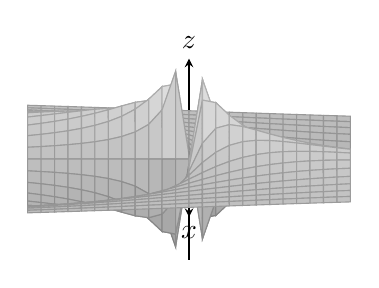
\begin{tikzpicture}[declare function={f(\x,\y)=2*\x*\y/((\x)^4+(\y)^2);}]
  \begin{axis}[view/h=90,small,axis lines=center,colormap={}{gray(0.2cm)=(0.6);gray(1cm)=(0.9);},enlargelimits=true,xlabel={$x$},ylabel={$y$},zlabel={$z$},hide y axis,xlabel style={anchor={north}},zlabel style={anchor=south},xtick={\empty},ytick={\empty},ztick={\empty}]
    \addplot3[surf,domain=-2:2,domain y=-1:1] { (x==0&&y==0) ?0 : f(x,y) } ;
  \end{axis}
\end{tikzpicture}
\end{subfigure}\hfill
\begin{subfigure}{0.45\textwidth}
\centering
\begin{tikzpicture}[declare function={f(\x,\y)=2*\x*\y/((\x)^4+(\y)^2);}]
  \begin{axis}[view/h=90,small,axis lines=center,colormap={kdark}{gray(0.2cm)=(0.6);gray(1cm)=(0.6);},enlargelimits=true,xlabel={$x$},ylabel={$y$},zlabel={$z$},xlabel style={anchor={west}},ylabel style={anchor=south west},zlabel style={anchor=south},xtick={\empty},ytick={\empty},ztick={\empty},hide z axis]
\addplot3[contour gnuplot={output point meta=rawz,number=10,labels=false,},samples=41,z filter/.code=\def\pgfmathresult{0},]{f(x,y)};
  \end{axis}
\end{tikzpicture}
\end{subfigure}
\caption{ماسوائے نقطہ \عددی{(0,0)} تفاعل \عددی{f(x,y)=2x^2y/(x^4+y^2)} استمراری ہے۔}
\label{شکل_مثال_کثیرالمتغیر_مبدا_پر_غیر_استمراری_سطح_ب}
\end{figure}
یہاں آپ سوال اٹھا سکتے ہیں کہ مبدا تک نقطہ \عددی{(x,y)} کے پہنچنے سے بہت سارے مختلف حد ملتے ہیں لہٰذا یہ کہنا درست نہیں کہ \عددی{f} کا حد غیر موجود ہے۔ یہی وہ نقطہ ہے جسے سمجھنا ضروری ہے۔ حد کی تعریف  کہتی ہے کہ حد کی قیمت راہ پر منحصر نہیں ہو سکتی۔

\جزوحصہء{دو سے زیادہ متغیرات کے تفاعل}
دو متغیرات کے تفاعل  کے حد اور استمرار کی تعریف  اور ان  تفاعل کے مجموعہ،  فرق، حاصل ضرب، حاصل تقسیم، طاقت اور مرکب کے بارے میں حاصل نتائج  تین یا تین سے زیادہ متغیرات کے تفاعل کے لئے بھی کارآمد  ہیں۔ درج ذیل تفاعل اپنے پورے دائرہ کار میں استمراری ہیں
\begin{align*}
\ln(x+y+z)\quad \text{اور}\quad \frac{y\sin z}{x-1}
\end{align*} 
اور  درج ذیل طرز کا حد ، جہاں \عددی{N} نقطہ \عددی{(x,y,z)} کو ظاہر کرتا ہے،   حاصل کرنے کے لئے  تفاعل میں نقطہ پر  کیا جاتا ہے۔
\begin{align*}
\lim_{N\to(1,0,-1)}\frac{e^{x+z}}{z^2+\cos\sqrt{xy}}=\frac{e^{1-1}}{(-1)^2+\cos 0}=\frac{1}{2}
\end{align*}

\جزوحصہء{سوالات}
\ابتدا{سوالات}
\موٹا{حد کی قیمت کی تلاش}\\
سوال \حوالہ{سوال_کثیرالمتغیر_حد_قیمت_تلاش_الف} تا سوال \حوالہ{سوال_کثیرالمتغیر_حد_قیمت_تلاش_ب} میں حد کی قیمت تلاش کریں۔

\ابتدا{سوال}\شناخت{سوال_کثیرالمتغیر_حد_قیمت_تلاش_الف}
$\lim\limits_{(x,y)\to(0,0)}\frac{3x^2-y^2+5}{x^2+y^2+2}$
\ابتدا{جواب}
\wf{\unexpanded{
$\tfrac{5}{2}$
}}
\انتہا{جواب}
\انتہا{سوال}
%==================
\ابتدا{سوال}
$\lim\limits_{(x,y)\to(0,4)}\frac{x}{\sqrt{y}}$
\انتہا{سوال}
%===================
\ابتدا{سوال}
$\lim\limits_{(x,y)\to(3,4)}\sqrt{x^2+y^2-1}$
\ابتدا{جواب}
\wf{\unexpanded{
$2\sqrt{6}$
}}
\انتہا{جواب}
\انتہا{سوال}
%===================
\ابتدا{سوال}
$\lim\limits_{(x,y)\to(2,-3)}\big(\frac{1}{x}+\frac{1}{y}\big)^2$
\انتہا{سوال}
%===================
\ابتدا{سوال}
$\lim\limits_{(x,y)\to(0,\pi/4)}\sec x\tan y$
\ابتدا{جواب}
\wf{\unexpanded{
$1$
}}
\انتہا{جواب}
\انتہا{سوال}
%===================
\ابتدا{سوال}
$\lim\limits_{(x,y)\to(0,0)}\cos\frac{x^2+y^3}{x+y+1}$
\انتہا{سوال}
%===================
\ابتدا{سوال}
$\lim\limits_{(x,y)\to(0,\ln 2)}e^{x-y}$
\ابتدا{جواب}
\wf{\unexpanded{
$\tfrac{1}{2}$
}}
\انتہا{جواب}
\انتہا{سوال}
%===================
\ابتدا{سوال}
$\lim\limits_{(x,y)\to(1,1)}\ln\abs{1+x^2y^2}$
\انتہا{سوال}
%===================
\ابتدا{سوال}
$\lim\limits_{(x,y)\to(0,0)} \frac{e^y\sin x}{x}$
\ابتدا{جواب}
\wf{\unexpanded{
$1$
}}
\انتہا{جواب}
\انتہا{سوال}
%===================
\ابتدا{سوال}
$\lim\limits_{(x,y)\to(1,1)}\cos\sqrt[3]{\abs{xy}-1}$
\انتہا{سوال}
%===================
\ابتدا{سوال}
$\lim\limits_{(x,y)\to(1,0)}\frac{x\sin y}{x^2+1}$
\ابتدا{جواب}
\wf{\unexpanded{
$0$
}}
\انتہا{جواب}
\انتہا{سوال}
%===================
\ابتدا{سوال}\شناخت{سوال_کثیرالمتغیر_حد_قیمت_تلاش_ب}
$\lim\limits_{(x,y)\to(\pi/2,0)}\frac{\cos y+1}{y-\sin x}$
\انتہا{سوال}
%===================

\موٹا{حاصل تقسیم کے حد}\\
حاصل تقسیم کو ترتیب دیتے ہوئے سوال \حوالہ{سوال_کثیرالمتغیر_ترتیب_حد_تلاش_الف} تا سوال \حوالہ{سوال_کثیرالمتغیر_ترتیب_حد_تلاش_ب} میں حد تلاش کریں۔

\ابتدا{سوال}\شناخت{سوال_کثیرالمتغیر_ترتیب_حد_تلاش_الف}
$\lim\limits_{\substack{(x,y)\to(1,1)\\ x\ne y}}\frac{x^2-2xy+y^2}{x-y}$
\ابتدا{جواب}
\wf{\unexpanded{
$0$
}}
\انتہا{جواب}
\انتہا{سوال}
%=================
\ابتدا{سوال}
$\lim\limits_{\substack{(x,y)\to(1,1)\\ x\ne y}}\frac{x^2-y^2}{x-y}$
\انتہا{سوال}
%=================
\ابتدا{سوال}
$\lim\limits_{\substack{(x,y)\to(1,1)\\x\ne 1}}\frac{xy-y-2x+2}{x-1}$
\ابتدا{جواب}
\wf{\unexpanded{
$-1$
}}
\انتہا{جواب}
\انتہا{سوال}
%=================
\ابتدا{سوال}
$\lim\limits_{\substack{(x,y)\to(2,-4)\\y\ne -4,\, x\ne x^2}}\frac{y+4}{x^2y-xy+4x^2-4x}$
\انتہا{سوال}
%=================
\ابتدا{سوال}
$\lim\limits_{\substack{(x,y)\to(0,0)\\x\ne y}}\frac{x-y+2\sqrt{x}-2\sqrt{y}}{\sqrt{x}-\sqrt{y}}$
\ابتدا{جواب}
\wf{\unexpanded{
$2$
}}
\انتہا{جواب}
\انتہا{سوال}
%=================
\ابتدا{سوال}
$\lim\limits_{\substack{(x,y)\to(2,2)\\x+y\ne 4}}\frac{x+y-4}{\sqrt{x+y}-2}$
\انتہا{سوال}
%=================
\ابتدا{سوال}
$\lim\limits_{\substack{(x,y)\to(2,0)\\2x-y\ne 4}}\frac{\sqrt{2x-y}-2}{2x-y-4}$
\ابتدا{جواب}
\wf{\unexpanded{
$\tfrac{1}{4}$
}}
\انتہا{جواب}
\انتہا{سوال}
%=================
\ابتدا{سوال}\شناخت{سوال_کثیرالمتغیر_ترتیب_حد_تلاش_ب}
$\lim\limits_{\substack{(x,y)\to(4,3)\\x\ne y+1}}\frac{\sqrt{x}-\sqrt{y+1}}{x-y-1}$
\انتہا{سوال}
%=================

\موٹا{تین متغیرات کے تفاعل کا حد}\\
سوال \حوالہ{سوال_کثیرالمتغیر_تین_متغیر_حد_الف} تا سوال \حوالہ{سوال_کثیرالمتغیر_تین_متغیر_حد_ب} میں حد تلاش کریں۔

\ابتدا{سوال}\شناخت{سوال_کثیرالمتغیر_تین_متغیر_حد_الف}
$\lim\limits_{N\to (1,3,4)}\big(\frac{1}{x}+\frac{1}{y}+\frac{1}{z}\big)$
\ابتدا{جواب}
\wf{\unexpanded{
$\tfrac{19}{12}$
}}
\انتہا{جواب}
\انتہا{سوال}
%=====================
\ابتدا{سوال}
$\lim\limits_{N\to(1,-1,-1)}\frac{2xy+yz}{x^2+z^2}$
\انتہا{سوال}
%================
\ابتدا{سوال}
$\lim\limits_{N\to(3,3,0)}(\sin^2x+\cos^2y+\sec^2z)$
\ابتدا{جواب}
\wf{\unexpanded{
$2$
}}
\انتہا{جواب}
\انتہا{سوال}
%======================
\ابتدا{سوال}
$\lim\limits_{N\to(-1/4,\pi/2,2)}\tan^{-1}xyz$
\انتہا{سوال}
%======================
\ابتدا{سوال}
$\lim\limits_{N\to(\pi,0,3)}ze^{-2y}\cos 2x$
\ابتدا{جواب}
\wf{\unexpanded{
$3$
}}
\انتہا{جواب}
\انتہا{سوال}
%======================
\ابتدا{سوال}\شناخت{سوال_کثیرالمتغیر_تین_متغیر_حد_ب}
$\lim\limits_{N\to(0,-2,0)}\ln\sqrt{x^2+y^2+z^2}$
\انتہا{سوال}
%======================

\موٹا{مستوی میں استمرار}\\
سوال \حوالہ{سوال_کثیرالمتغیر_استمراری_سطح_الف} تا سوال \حوالہ{سوال_کثیرالمتغیر_استمراری_سطح_ب} میں  کس نقطہ \عددی{(x,y)} پر مستوی میں تفاعل استمراری ہیں؟

\ابتدا{سوال}\شناخت{سوال_کثیرالمتغیر_استمراری_سطح_الف}
(ا)
$f(x,y)=\sin(x+y)$\quad
(ب)
$f(x,y)=\ln(x^2+y^2)$
\ابتدا{جواب}
\wf{\unexpanded{
(ا)   تمام \عددی{(x,y)}، (ب) ماسوائے \عددی{(0,0)} تمام \عددی{(x,y)}
}}
\انتہا{جواب}
\انتہا{سوال}
%==================
\ابتدا{سوال}
(ا)
$f(x,y)=\frac{x+y}{x-y}$\quad
(ب)
$f(x,y)=\frac{y}{x^2+1}$
\انتہا{سوال}
%=================
\ابتدا{سوال}
(ا)
$g(x,y)=\sin\frac{1}{xy}$\quad
(ب)
$g(x,y)=\frac{x+y}{2+\cos x}$
\ابتدا{جواب}
\wf{\unexpanded{
(ا) تمام \عددی{(x,y)} ماسوائے جہاں \عددی{x=0} یا \عددی{y=0} ہو، (ب) تمام \عددی{(x,y)}
}}
\انتہا{جواب}
\انتہا{سوال}
%=================
\ابتدا{سوال}\شناخت{سوال_کثیرالمتغیر_استمراری_سطح_ب}
(ا)
$g(x,y)=\frac{x^2+y^2}{x^2-3x+2}$\quad
(ب)
$g(x,y)=\frac{1}{x^2-y}$
\انتہا{سوال}
%=================

\موٹا{فضا میں استمرار}\\
سوال \حوالہ{سوال_کثیرالمتغیر_استمراری_فضا_الف} تا سوال \حوالہ{سوال_کثیرالمتغیر_استمراری_فضا_ب} میں  کس نقطہ \عددی{(x,y,z)} پر فضا  میں تفاعل استمراری ہیں؟

\ابتدا{سوال}\شناخت{سوال_کثیرالمتغیر_استمراری_فضا_الف}
(ا)
$f(x,y,z)=x^2+y^2-2z^2$\quad
(ب)
$f(x,y,z)=\sqrt{x^2+y^2-1}$
\ابتدا{جواب}
\wf{\unexpanded{
(ا) تمام \عددی{(x,y,z)}، (ب) نلکی \عددی{x^2+y^2=1} کی اندرون کے علاوہ تمام \عددی{(x,y,z)}
}}
\انتہا{جواب}
\انتہا{سوال}
%=================
\ابتدا{سوال}
(ا)
$f(x,y,z)=\ln xyz$\quad
(ب)
$f(x,y,z)=e^{x+y}\cos z$
\انتہا{سوال}
%=====================
\ابتدا{سوال}
(ا)
$h(x,y,z)=xy\sin\frac{1}{z}$\quad
(ب)
$h(x,y,z)=\frac{1}{x^2+z^2-1}$
\ابتدا{جواب}
\wf{\unexpanded{
(ا) وہ تمام \عددی{(x,y,z)} جہاں \عددی{z\ne 0} ہو، (ب)   وہ تمام \عددی{(x,y,z)} جہاں \عددی{x^2+y^2\ne 1} ہو۔
}}
\انتہا{جواب}
\انتہا{سوال}
%=====================
\ابتدا{سوال}\شناخت{سوال_کثیرالمتغیر_استمراری_فضا_ب}
(ا)
$h(x,y,z)=\frac{1}{\abs{y}+\abs{z}}$\quad
(ب)
$h(x,y,z)=\frac{1}{\abs{xy}+\abs{z}}$
\انتہا{سوال}
%=====================

\موٹا{نقطہ پر حد غیر موجود}\\
نقطہ تک   مختلف راہ پر پہنچتے ہوئے سوال \حوالہ{سوال_کثیرالمتغیر_غیر_موجود_حد_الف} تا سوال \حوالہ{سوال_کثیرالمتغیر_غیر_موجود_حد_ب} میں دکھائیں کہ \عددی{(x,y)\to(0,0)} کرتے ہوئے تفاعل کا کوئی حد نہیں پایا جاتا ہے۔

\ابتدا{سوال}\شناخت{سوال_کثیرالمتغیر_غیر_موجود_حد_الف}
$f(x,y)=-\frac{x}{\sqrt{x^2+y^2}}$\quad
(شکل \حوالہ{شکل_سوال_کثیرالمتغیر_غیر_موجود_حد_الف}-ا)
\ابتدا{جواب}
\wf{\unexpanded{
راہ \عددی{y=x,x>0} اور \عددی{y=x,x<0}  لیں۔ 
}}
\انتہا{جواب}
\انتہا{سوال}
%===================
\begin{figure}
\centering
\begin{subfigure}{0.45\textwidth}
\centering
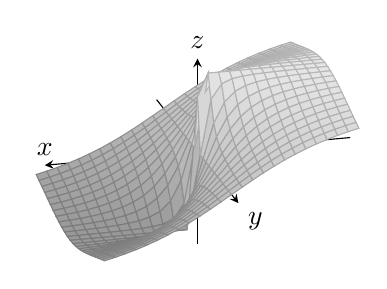
\begin{tikzpicture}[declare function={f(\x,\y)=-\x/sqrt((\x)^2+(\y)^2);}]
\begin{axis}[small,axis lines=center,view/h=165,colormap={}{gray(0.2cm)=(0.6);gray(1cm)=(0.9);},enlargelimits=true,xlabel={$x$},ylabel={$y$},zlabel={$z$},xlabel style={anchor=south},ylabel style={anchor=north west},zlabel style={anchor=south},xtick={\empty},ytick={\empty},ztick={\empty}]
\addplot3[z buffer=sort,surf,domain=-0.1:0.1,domain y=-0.1:0.1]{f(x,y)};
\end{axis}
\end{tikzpicture}
\caption{}
\end{subfigure}\hfill
\begin{subfigure}{0.45\textwidth}
\centering
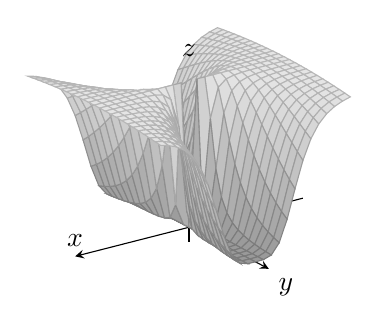
\begin{tikzpicture}[declare function={f(\x,\y)=(\x)^4/((\x)^4+(\y)^2);}]
\begin{axis}[small,axis lines=center,view/h=145,colormap={}{gray(0.2cm)=(0.6);gray(1cm)=(0.9);},enlargelimits=true,xlabel={$x$},ylabel={$y$},zlabel={$z$},xlabel style={anchor=south},ylabel style={anchor=north west},zlabel style={anchor=south},xtick={\empty},ytick={\empty},ztick={\empty}]
\addplot3[z buffer=sort,surf]{f(x,y)};
\end{axis}
\end{tikzpicture}
\caption{}
\end{subfigure}
\caption{}
\label{شکل_سوال_کثیرالمتغیر_غیر_موجود_حد_الف}
\end{figure}
\ابتدا{سوال}
$h(x,y)=\frac{x^4}{x^4+y^2}$\quad
(شکل \حوالہ{شکل_سوال_کثیرالمتغیر_غیر_موجود_حد_الف}-ب)
\انتہا{سوال}
%=================
\ابتدا{سوال}
$h(x,y)=\frac{x^4-y^2}{x^4+y^2}$
\ابتدا{جواب}
\wf{\unexpanded{
راہ \عددی{y=kx^2} لیں جہاں \عددی{k} ایک  مستقل ہو۔
}}
\انتہا{جواب}
\انتہا{سوال}
%================
\ابتدا{سوال}
$f(x,y)=\frac{xy}{\abs{xy}}$
\انتہا{سوال}
%=================
\ابتدا{سوال}
$g(x,y)=\frac{x-y}{x+y}$
\ابتدا{جواب}
\wf{\unexpanded{
راہ \عددی{y=mx} لیں جہاں \عددی{m} ایک مستقل    \عددی{m\ne -1} ہو۔
}}
\انتہا{جواب}
\انتہا{سوال}
%=================
\ابتدا{سوال}
$g(x,y)=\frac{x+y}{x-y}$
\انتہا{سوال}
%=================
\ابتدا{سوال}
$h(x,y)=\frac{x^2+y}{y}$
\ابتدا{جواب}
\wf{\unexpanded{
راہ \عددی{y=kx^2} لیں جہاں \عددی{k} ایک مستقل  \عددی{k\ne 0} ہو۔ 
}}
\انتہا{جواب}
\انتہا{سوال}
%=================
\ابتدا{سوال}\شناخت{سوال_کثیرالمتغیر_غیر_موجود_حد_ب}
$h(x,y)=\frac{x^2}{x^2-y}$
\انتہا{سوال}
%=================
\موٹا{نظریہ اور مثالیں}\\
\ابتدا{سوال}
کیا  \عددی{\lim_{(x,y)\to(x_0,y_0)}f(x,y)=L} کی صورت میں \عددی{(x_0,y_0)} کا معین ہونا لازمی ہے؟ اپنے جواب کی وجہ پیش کریں۔
\ابتدا{جواب}
\wf{\unexpanded{
نہیں
}}
\انتہا{جواب}
\انتہا{سوال}
%=====================
\ابتدا{سوال}
اگر \عددی{f(x_0,y_0)=3} ہو تب درج ذیل کے بارے میں  (ا)   \عددی{(x_0,y_0)} پر استمراری \عددی{f} کی صورت میں،
\begin{align*}
\lim_{(x,y)\to(x_0,y_0)} f(x,y)
\end{align*}
(ب)  \عددی{(x_0,y_0)} پر غیر استمراری \عددی{f} کی صورت میں کیا کہا جا  سکتا ہے۔ اپنے جواب کہ وجہ پیش کریں۔
\انتہا{سوال}
%===============
دو متغیرات کے تفاعل کا مسئلہ بیچ  کہتا ہے کہ اگر ایک قرص، جس کا  مرکز  \عددی{(x_0,y_0)} ہو، کے اندر تمام \عددی{(x,y)\ne (x_0,y_0)} پر \عددی{g(x,y)\le f(x,y)\le h(x,y)} ہو،  اور \عددی{(x,y)\to (x_0,y_0)} کرتے ہوئے  \عددی{g} اور \عددی{h} دونوں کا  حد  متناہی اور \عددی{L} ہو   تب
\begin{align*}
\lim_{(x,y)\to(x_0,y_0)}f(x,y)=L
\end{align*}
ہو گا۔سوال \حوالہ{سوال_کثیرالمتغیر_مسئلہ_بیچ_الف} تا سوال \حوالہ{سوال_کثیرالمتغیر_مسئلہ_بیچ_ب} میں  اس نتیجہ  کا سہارا لیتے ہوئے جواب دیں۔ 

\ابتدا{سوال}\شناخت{سوال_کثیرالمتغیر_مسئلہ_بیچ_الف}
کیا 
\begin{align*}
1-\frac{x^2y^2}{3}<\frac{\tan^{-1}xy}{xy}<1
\end{align*}
جانتے ہوئے آپ
\begin{align*}
\lim\limits_{(x,y)\to(0,0)}\frac{\tan^{-1}xy}{xy}
\end{align*}
کے بارے میں کچھ کہہ سکتے ہیں؟ اپنے جواب کی وجہ پیش کریں۔
\ابتدا{جواب}
\wf{\unexpanded{
حد \عددی{1} ہے۔
}}
\انتہا{جواب}
\انتہا{سوال}
%============
\ابتدا{سوال}
کیا
\begin{align*}
2\abs{xy}-\frac{x^2y^2}{6}<4-4\cos\sqrt{\abs{xy}}<2\abs{xy}
\end{align*}
جانتے ہوئے
\begin{align*}
\lim\limits_{(x,y)\to(0,0)}\frac{4-4\cos\sqrt{\abs{xy}}}{\abs{xy}}
\end{align*}
کے بارے میں کچھ کہا جا سکتا ہے؟ اپنے جواب کی وجہ پیش کریں۔
\انتہا{سوال}
%===============
\ابتدا{سوال}
کیا \عددی{\abs{\sin(1/x)}\le 1} جانتے ہوئے درج ذیل کے بارے میں کچھ کہا جا سکتا ہے؟ اپنے جواب کی وجہ پیش کریں۔
\begin{align*}
\lim\limits_{(x,y)\to(0,0)}y\sin\frac{1}{x}
\end{align*}
\ابتدا{جواب}
\wf{\unexpanded{
حد \عددی{0} ہے۔
}}
\انتہا{جواب}
\انتہا{سوال}
%==============
\ابتدا{سوال}
کیا \عددی{\abs{\cos(1/y)}\le 1} جانتے ہوئے درج ذیل کے بارے میں کچھ کہا جا سکتا ہے؟ اپنے جواب کی وجہ پیش کریں۔
\begin{align*}
\lim\limits_{(x,y)\to(0,0)}x\cos\frac{1}{y}
\end{align*}
\انتہا{سوال}
%==============
\ابتدا{سوال}
(ا)دوبارہ  مثال \حوالہ{مثال_کثیرالمتغیر_حد_یکتا_ضروری} کو  پڑھیں۔اب درج ذیل کلیہ میں \عددی{m=\tan\theta} پر کر کے اس کی سادہ صورت حاصل کرتے ہوئے دکھائیں کہ \عددی{f} کی قیمت  لکیر کے زاویہ میلان  پر منحصر ہی گی۔
\begin{align*}
\left.f(x,y)\right\vert_{y=mx}=\frac{2m}{1+m^2}
\end{align*}
(ب) جزو-ا میں حاصل کلیہ استعمال کرتے ہوئے دکھائیں کہ لکیر \عددی{y=mx} پر چلتے ہوئے \عددی{(x,y)\to (0,0)} کرنے سے \عددی{f} کے  حد کی قیمت \عددی{-1} تا \عددی{1} ہو سکتی ہے جو قریب پہنچنے کی راہ کے  زاویہ پر منحصر ہو گی۔  
\ابتدا{جواب}
\wf{\unexpanded{
(ا) \عددی{\left. f(x,y)\right\vert_{y=mx}=\sin2\theta} جہاں\\  
 \عددی{\tan\theta=m} ہے۔
}}
\انتہا{جواب}
\انتہا{سوال}
%=================
\ابتدا{سوال}\شناخت{سوال_کثیرالمتغیر_مسئلہ_بیچ_ب}
\عددی{f(0,0)} کی ایسی تعریف پیش کریں جو درج ذیل کو مبدا پر بھی استمراری بناتا ہو۔
\begin{align*}
f(x,y)=xy\frac{x^2-y^2}{x^2+y^2}
\end{align*}
\انتہا{سوال}
%==============

\موٹا{قطبی محدد میں تبادلہ}\\
اگر کارتیسی محدد میں \عددی{\lim_{(x,y)\to(0,0)}f(x,y)}  کے حصول میں پیش رفت  نہ ہو تب قطبی محدد میں حد تلاش کرنے کی کوشش کریں۔ ایسا کرنے  کی خاطر \عددی{x=r\cos\theta} اور \عددی{y=r\sin\theta} کرتے ہوئے \عددی{r\to 0}  کے لئے حاصل تفاعل کا حد تلاش کریں۔دوسرے الفاظ میں یہ دیکھنے کی کوشش کریں کہ آیا کوئی ایسا عدد \عددی{L} پایا جاتا ہے جو درج ذیل کو مطمئن کرتا ہو:

کسی بھی دیے گئے عدد \عددی{\epsilon>0} کا ایسا مطابقتی عدد \عددی{\delta>0} پایا جاتا ہو کہ تمام \عددی{r} اور \عددی{\theta} کے لئے درج ذیل ہو۔
\begin{align*}
\abs{r}<\delta\implies \abs{f(r,\theta)-L}<\epsilon
\end{align*}
اگر ایسا \عددی{L} موجود ہو تب
\begin{align}\label{مساوات_کثیرالمتغیر_قطبی_حد_الف}
\lim_{(x,y)\to(0,0)}f(x,y)=\lim_{r\to 0}f(r,\theta)=L
\end{align}
ہو گا۔مثال کے طور پر 
\begin{align*}
\lim_{(x,y)\to(0,0)}\frac{x^3}{x^2+y^2}=\lim_{r\to 0}\frac{r^3\cos^3\theta}{r^2}=\lim_{r\to 0}r\cos^3\theta=0
\end{align*}
ہو گا۔ آخری عدم مساوات  کی تصدیق کرنے کی خاطر ہمیں دکھانا  ہو گا کہ \عددی{f(r,\theta)=r\cos^3\theta} اور \عددی{L}  مساوات \حوالہ{مساوات_کثیرالمتغیر_قطبی_حد_الف} کو مطمئن کرتے ہیں۔ یعنی ہمیں دکھانا ہو گا کہ کسی بھی دیے گئے عدد \عددی{\epsilon>0} کے لئے ایسا مطابقتی  عدد \عددی{\delta>0} موجود ہے کہ  تمام \عددی{r} اور \عددی{\theta} کے لئے درج ذیل  مطمئن ہو۔
\begin{align}\label{مساوات_کثیرالمتغیر_قطبی_حد_ب}
\abs{r}<\delta\implies \abs{r\cos^3\theta-0}<\epsilon
\end{align}
چونکہ
\begin{align*}
\abs{r\cos^3\theta}=\abs{r}\abs{\cos^3\theta}\le \abs{r}\cdot 1=\abs{r}
\end{align*}
ہوتا ہے لہٰذا  \عددی{\delta=\epsilon} لینے سے تمام \عددی{r} اور \عددی{\theta} کے لئے مساوات \حوالہ{مساوات_کثیرالمتغیر_قطبی_حد_ب} مطمئن ہو گا۔

اس کے برعکس    \عددی{\abs{r}} جتنا بھی چھوٹا کیوں نا ہو   درج ذیل تفاعل کی قیمت \عددی{0}  سے  \عددی{1} تک ہو سکتی ہے لہٰذا \عددی{\lim_{(x,y)\to (0,0)}\tfrac{x^2}{x^2+y^2}} غیر موجود ہو گا۔
\begin{align*}
\frac{x^2}{x^2+y^2}=\frac{r^2\cos^2\theta}{r^2}=\cos^2\theta
\end{align*}

درج بالا دو تفاعل میں \عددی{r\to 0} کرتے ہوئے  حد کی موجودگی یا غیر موجودگی کا مسئلہ سیدھا تھا۔البتہ ضروری نہیں کہ  قطبی محدد میں تبادلہ سودمند ثابت ہو، بلکہ بعض اوقات ایسا کرنے سے ہم بالکل غلط نتیجہ کی طرف راغب ہو سکتے ہیں۔ مثال کے طور پر، تمام سیدھے خطوط \عددی{\theta=c}، جہاں \عددی{c} مستقل ہے، پر حد موجود ہو سکتا ہے اگرچہ وسیع معنوں میں حد غیر موجود ہو گا۔ مثال \حوالہ{مثال_کثیرالمتغیر_مبدا_پر_غیر_استمراری_سطح_ب} میں اس حقیقت کی وضاحت کی گئی ہے۔قطبی محدد میں \عددی{r\ne 0} کے لئے  \عددی{f(x,y)=\tfrac{2x^2y}{x^4+y^2}} درج ذیل ہو گا۔
\begin{align*}
f(r\cos\theta,r\sin\theta)=\frac{r\cos\theta\sin2\theta}{r^2\cos^4\theta+\sin^2\theta}
\end{align*}
اب \عددی{\theta}  برقرار رکھتے ہوئے  \عددی{r\to 0} کرنے سے حد \عددی{0} ملتا ہے۔البتہ راہ \عددی{y=x^2} پر \عددی{r\sin\theta=r^2\cos^2\theta}لہٰذا درج ذیل ہو گا۔
\begin{align*}
f(r\cos\theta,r\sin\theta)&=\frac{r\cos\theta\sin 2\theta}{r^2\cos^4\theta+(r\cos^2\theta)^2}\\
&=\frac{2r\cos^2\theta\sin\theta}{2r^2\cos^4\theta}=\frac{r\sin\theta}{r^2\cos^2\theta}=1
\end{align*}

سوال \حوالہ{سوال_کثیرالمتغیر_قطبی_محدد_حد_الف} تا سوال \حوالہ{سوال_کثیرالمتغیر_قطبی_محدد_حد_ب} میں \عددی{(x,y)\to(0,0)} کرتے ہوئے \عددی{f} کا حد تلاش کریں یا دکھائیں کہ اس کا حد غیر موجود ہے۔

\ابتدا{سوال}\شناخت{سوال_کثیرالمتغیر_قطبی_محدد_حد_الف}
$f(x,y)=\frac{x^3-xy^2}{x^2+y^2}$
\ابتدا{جواب}
\wf{\unexpanded{
$0$
}}
\انتہا{جواب}
\انتہا{سوال}
%==================
\ابتدا{سوال}
$f(x,y)=\cos\big(\frac{x^3-y^3}{x^2+y^2}\big)$
\انتہا{سوال}
%====================
\ابتدا{سوال}
$f(x,y)=\frac{y^2}{x^2+y^2}$
\ابتدا{جواب}
\wf{\unexpanded{
غیر موجود ہے۔
}}
\انتہا{جواب}
\انتہا{سوال}
%====================
\ابتدا{سوال}
$f(x,y)=\frac{2x}{x^2+x+y^2}$
\انتہا{سوال}
%====================
\ابتدا{سوال}
$f(x,y)=\tan^{-1}\big(\frac{\abs{x}+\abs{y}}{x^2+y^2}\big)$
\ابتدا{جواب}
\wf{\unexpanded{
$\tfrac{\pi}{2}$
}}
\انتہا{جواب}
\انتہا{سوال}
%====================
\ابتدا{سوال}\شناخت{سوال_کثیرالمتغیر_قطبی_محدد_حد_ب}
$f(x,y)=\frac{x^2-y^2}{x^2+y^2}$
\انتہا{سوال}
%====================

سوال \حوالہ{سوال_کثیرالمتغیر_مبدا_پر_استمراری_الف} اور سوال \حوالہ{سوال_کثیرالمتغیر_مبدا_پر_استمراری_ب} میں \عددی{f(0,0)} کی ایسی تعریف پیش کریں کہ \عددی{f} مبدا پر بھی استمراری ہو۔

\ابتدا{سوال}\شناخت{سوال_کثیرالمتغیر_مبدا_پر_استمراری_الف}
$f(x,y)=\ln\big(\frac{3x^2-x^2y^2+3y^2}{x^2+y^2}\big)$
\ابتدا{جواب}
\wf{\unexpanded{
$f(0,0)=\ln 3$
}}
\انتہا{جواب}
\انتہا{سوال}
%====================
\ابتدا{سوال}\شناخت{سوال_کثیرالمتغیر_مبدا_پر_استمراری_ب}
$f(x,y)=\frac{2xy^2}{x^2+y^2}$
\انتہا{سوال}
%=================

\موٹا{\عددی{\delta\epsilon}  تعریفات  کا استعمال}\\
\ابتدا{سوال}
دکھائیں کہ حد کی تعریف  (مساوات \حوالہ{مساوات_کثیرالمتغیر_تعریف_حد_الف}) میں \عددی{\delta\epsilon} پر عائد  شرط مساوات \حوالہ{مساوات_کثیرالمتغیر_تعریف_حد_ب} میں دی گئی شرط کے مترادف ہے۔
\انتہا{سوال}
%===================
\ابتدا{سوال}
\عددی{(x,y)\to (x_0,y_0)} کرتے ہوئے تفاعل \عددی{f(x,y)}کے حد  کی باضابطہ \عددی{\delta\epsilon} تعریف کو مد نظر رکھتے ہوئے  \عددی{(x,y,z)\to(x_ 0,y_0,z_0)} کرتے ہوئے \عددی{g(x,y,z)} کے حد کی تعریف پیش کریں۔چار غیر تابع متغیرات کے تفاعل \عددی{h(x,y,z,t)} کی حد کی تعریف کیا ہو گی؟  
\انتہا{سوال}
%=========

سوال \حوالہ{سوال_کثیرالمتغیر_حد_دو_متغیرات_الف} تا سوال \حوالہ{سوال_کثیرالمتغیر_حد_دو_متغیرات_ب} میں  تفاعل \عددی{f(x,y)} اور مثبت عدد \عددی{\epsilon} دیے گئے ہیں۔ ہر ایک سوال میں یا دکھائیں کہ  ایسا \عددی{\delta>0} موجود ہے  کہ  \عددی{(x,y)} کے لئے 
\begin{align*}
\sqrt{x^2+y^2}<\delta\implies \abs{f(x,y)-f(0,0)}<\epsilon
\end{align*}
مطمئن ہوتا ہے  یا دکھائیں کہ ایسا \عددی{\delta>0} موجود ہے کہ تمام \عددی{(x,y)} کے لئے
\begin{align*}
\abs{x}<\delta,\quad \abs{y}<\delta \implies \abs{f(x,y)-f(0,0)}<\epsilon
\end{align*}
مطمئن ہوتا ہے۔ان میں سے وہ دکھائیں  جو آپ کو زیادہ  آسان لگے۔ دونوں دکھانے  کی ضرورت نہیں ہے۔ 

\ابتدا{سوال}\شناخت{سوال_کثیرالمتغیر_حد_دو_متغیرات_الف}
$f(x,y)=x^2+y^2,\quad \epsilon=0.01$
\ابتدا{جواب}
\wf{\unexpanded{
$\delta=0.1$
}}
\انتہا{جواب}
\انتہا{سوال}
%==================
\ابتدا{سوال}
$f(x,y)=\frac{y}{x^2+1},\quad \epsilon=0.05$
\انتہا{سوال}
%==============
\ابتدا{سوال}
$f(x,y)=\frac{x+y}{x^2+1},\quad \epsilon=0.01$
\ابتدا{جواب}
\wf{\unexpanded{
$\delta=0.005$
}}
\انتہا{جواب}
\انتہا{سوال}
%================
\ابتدا{سوال}\شناخت{سوال_کثیرالمتغیر_حد_دو_متغیرات_ب}
$f(x,y)=\frac{x+y}{2+\cos x},\quad \epsilon=0.02$
\انتہا{سوال}
%=================


سوال \حوالہ{سوال_کثیرالمتغیر_حد_تین_متغیرات_الف} تا سوال \حوالہ{سوال_کثیرالمتغیر_حد_تین_متغیرات_ب} میں  تفاعل \عددی{f(x,y,z)} اور مثبت عدد \عددی{\epsilon} دیے گئے ہیں۔ ہر ایک سوال میں یا دکھائیں کہ  ایسا \عددی{\delta>0} موجود ہے  کہ  \عددی{(x,y,z)} کے لئے 
\begin{align*}
\sqrt{x^2+y^2+z^2}<\delta\implies \abs{f(x,y,z)-f(0,0,0)}<\epsilon
\end{align*}
مطمئن ہوتا ہے  یا دکھائیں کہ ایسا \عددی{\delta>0} موجود ہے کہ تمام \عددی{(x,y,z)} کے لئے
\begin{align*}
\abs{x}<\delta,\quad \abs{y}<\delta,\quad \abs{z}<\delta  \implies \abs{f(x,y,z)-f(0,0,0)}<\epsilon
\end{align*}
مطمئن ہوتا ہے۔ان میں سے وہ دکھائیں  جو آپ کو زیادہ  آسان لگے۔ دونوں دکھانے کی ضرورت نہیں ہے۔ 

\ابتدا{سوال}\شناخت{سوال_کثیرالمتغیر_حد_تین_متغیرات_الف}
$f(x,y,z)=x^2+y^2+z^2,\quad \epsilon=0.015$
\ابتدا{جواب}
\wf{\unexpanded{
$\delta=\sqrt{0.015}$
}}
\انتہا{جواب}
\انتہا{سوال}
%=================
\ابتدا{سوال}
$f(x,y,z)=xyz,\quad \epsilon=0.008$
\انتہا{سوال}
%===================
\ابتدا{سوال}
$f(x,y,z)=\frac{x+y+z}{x^2+y^2+z^2+1},\quad \epsilon=0.015$
\ابتدا{جواب}
\wf{\unexpanded{
$\delta=0.005$
}}
\انتہا{جواب}
\انتہا{سوال}
%===================
\ابتدا{سوال}\شناخت{سوال_کثیرالمتغیر_حد_تین_متغیرات_ب}
$f(x,y,z)=\tan^2x+\tan^2y+\tan^2z,\quad \epsilon=0.03$
\انتہا{سوال}
%===================
\ابتدا{سوال}
دکھائیں کہ ہر نقطہ  \عددی{(x_0,y_0,z_0)} پر تفاعل \عددی{f(x,y,z)=x+y-z} استمراری ہے۔ 
\انتہا{سوال}
%===============
\ابتدا{سوال}
دکھائیں کہ مبدا پر \عددی{f(x,y,z)=x^2+y^2+z^2} استمراری ہے۔
\انتہا{سوال}
%==================
\انتہا{سوالات}


\حصہ{جزوی تفرقات}
جب  ماسوائے ایک غیر تابع متغیر کے ہم باقی تمام  کو برقرار رکھیں اور اس ایک متغیر کے لحاظ سے تفاعل کا تفرق لیں تو ہمیں "جزوی" تفرق حاصل ہوتا ہے۔ اس حصہ میں دکھایا جائے گا کہ جزوی تفرقات کیسے  پائے جاتے ہیں اور واحد متغیر کے تفاعل کے تفرق کے قواعد بروئے کار لاتے ہوئے   جزوی تفرقات   کی قیمت کے حصول کے بارے میں بتایا جائے گا۔

\جزوحصہء{تعریفات اور علامتیت }
اگر تفاعل \عددی{f(x,y)} کے دائرہ کار میں \عددی{(x_0,y_0)} ایک نقطہ ہو تب انتصابی سطح \عددی{y=y_0}  سطح \عددی{z=f(x,y)} کو منحنی \عددی{z=f(x,y_0)} میں مس کرے گا (شکل \حوالہ{شکل_کثیرالمتغیر_تقاطع_سطح_اور_مستوی})۔ یہ منحنی مستوی \عددی{y=y_0} میں   تفاعل \عددی{z=f(x,y_0)} کی ترسیم ہو گی۔اس مستوی میں  افقی محدد \عددی{x}  ہے؛   انتصابی محدد \عددی{z} ہے۔
\begin{figure}
\centering
\pgfmathsetmacro{\xa}{1}
\pgfmathsetmacro{\ya}{1.25}
\pgfmathsetmacro{\m}{-3*\xa^2}
\pgfmathsetmacro{\za}{8-\xa^3}
\pgfmathsetmacro{\xb}{\xa+0.4}
\begin{tikzpicture}[declare function={f(\x,\y)=8-(\x)^3;g(\x)=\za+\m*(\x-\xa);}]
\begin{axis}[font=\small,clip=false,view/h=155,small,axis lines=center,xlabel={$x$},ylabel={$y$},zlabel={$z$},enlargelimits=true,zmax=9,colormap={lgray}{gray(0.2cm)=(0.9);gray(1cm)=(0.9);},xtick={\empty},ytick={\empty},ztick={\empty},xlabel style={anchor=north east},ylabel style={anchor=north west},zlabel style={anchor=east}]
\addplot3[surf,domain=0:1.75,domain y=0.4:2]{f(x,y)};
\addplot3[black,domain=0:1.75,samples y=0](x,\ya,{f(x,\ya)})node[pin={[align=right]-135:{\RL{مستوی \عددی{y=y_0} میں}\\  \RL{منحنی \عددی{z=f(x,y_0)}}}}]{};
\addplot3[black,domain=-0.2:1.75,samples y=0](x,\ya,{g(x)})node[pos=0,right]{\RL{مماسی خط}};
\addplot3[-latex]coordinates {(0,\ya,0)(1.75,\ya,0)}node[pos=0.3,pin={[below,align=right,font=\small,pin edge=-]-60:{\RL{مستوی \عددی{y=y_0} }\\  \RL{میں افقی محور}}}]{};
\addplot3[-latex]coordinates {(0,\ya,0)(0,\ya,12)}node[pos=0,below]{$y_0$}node[pos=0.15,pin={[align=right,font=\small,pin edge=-]45:{\RL{مستوی \عددی{y=y_0} }\\  \RL{میں انتصابی  محور}}}]{};
\addplot3[dashed]coordinates{(\xa,\ya,{f(\xa,\ya)})(\xa,\ya,0)}node[below]{$(x_0,y_0)$};
\addplot3[dashed]coordinates{(\xb,\ya,{f(\xb,\ya)})(\xb,\ya,0)}node[pin={[pin edge={-,solid},below]-110:{$(x_0+h,y_0)$}}]{};
\addplot3[]coordinates{(\xa,\ya,{f(\xa,\ya)})}node[pin=125:{$N(x_0,y_0,f(x_0,y_0))$}]{};
\addplot3[]coordinates {(1.75,0.4,{f(1.75,0.4)})}node[pin=170:{$z=f(x,y)$}]{};
\end{axis}
\end{tikzpicture}
\caption{مستوی \عددی{y=y_0} اور سطح \عددی{z=f(x,y)} کا تقاطع۔}
\label{شکل_کثیرالمتغیر_تقاطع_سطح_اور_مستوی}
\end{figure}

ہم نقطہ \عددی{(x_0,y_0)} پر \عددی{x} کے لحاظ سے \عددی{f} کے جزوی تفرق سے مراد  نقطہ \عددی{x=x_0} پر  \عددی{f(x,y_0)} کا سادہ تفرق لیتے ہیں۔

\ابتدا{تعریف}
نقطہ \عددی{(x_0,y_0)} پر\اصطلاح{ \عددی{x} کے لحاظ سے \عددی{f(x,y)} کا جزوی تفرق}\فرہنگ{تفرق!جزوی}\حاشیہب{partial derivative}\فرہنگ{derivative!partial}
\begin{align}\label{مساوات_کثیرالمتغیر_جزوی_تفرق_الف}
\left.\frac{\partial f}{\partial x}\right\vert_{(x_0,y_0)}=\left.\frac{\dif}{\dif x}f(x,y_0)\right\vert_{x=x_0}=\lim_{h\to 0}\frac{f(x_0+h,y_0)-f(x_0,y_0)}{h}
\end{align}
ہو گا بشرطیکہ  یہ حد موجود ہو۔ (آپ \عددی{\partial} کو \عددی{\dif} کی ایک قسم تصور کریں۔)
\انتہا{تعریف}
%================

نقطہ \عددی{N(x_0,y_0,f(x_0,y_0))} پر مستوی \عددی{y=y_0} میں منحنی \عددی{z=f(x,y_0)} کی ڈھلوان  سے مراد نقطہ \عددی{(x_0,y_0)} پر \عددی{x} کے لحاظ سے \عددی{f} کے جزوی تفرق کی قیمت ہے۔  نقطہ \عددی{N} پر منحنی کا مماسی خط، مستوی \عددی{y=y_0} میں وہ خط ہے جو \عددی{N} سے گزرتا ہو اور جس کی ڈھلوان یہی ہو۔ جب \عددی{y} کی قیمت برقرار \عددی{y_0} رکھی جائے  تب \عددی{x} کے لحاظ سے \عددی{f} کی شرح تبدیلی نقطہ \عددی{(x_0,y_0)} پر جزوی تفرق \عددی{\tfrac{\partial f}{\partial x}}    دیتا ہے۔ یہ نقطہ \عددی{(x_0,y_0)} پر \عددی{\ai} کے رخ \عددی{f} کی شرح تبدیلی  ہے۔

جزوی تفرق کی علامت اس چیز  پر منحصر ہو گی جس پر ہم زور دینا چاہتے ہیں۔یوں درج ذیل علامت اس وقت استعمال کیے جائیں گے  جب ہم نقطہ \عددی{(x_0,y_0)} پر زور دینا چاہیں۔
\begin{align*}
\frac{\partial f}{\partial x}(x_0,y_0),\quad f_x(x_0,y_0)
\end{align*}
سائنس اور انجینئری میں درج ذیل علامت مقبول ہے جہاں تفاعل کا صریحاً  ذکر  کیے  بغیر نقطہ \عددی{(x_0,y_0)} پر \عددی{x} کے لحاظ سے  \عددی{z} کا  جزوی تفرق لیا  گیا ہے۔
\begin{align*}
\left.\frac{\partial z}{\partial x}\right\vert_{(x_0,y_0)}
\end{align*}
جہاں جزوی تفرق  کو ایک تفاعل تصور کرنا مقصود  ہو وہاں درج ذیل علامت استعمال کیے جائیں گے، جہاں  \عددی{x} لے لحاظ سے \عددی{f} (یا \عددی{z}) کے جزوی تفرقات لیے گئے ہیں۔
\begin{align*}
f_x,\quad \frac{\partial f}{\partial x},\quad z_x,\quad \frac{\partial z}{\partial x}
\end{align*}

نقطہ \عددی{(x_0,y_0)} پر \عددی{y} کے لحاظ سے \عددی{f(x,y)} کے جزوی تفرق کی تعریف ، \عددی{x} کے لحاظ سے \عددی{f} کی جزوی تفرق کی تعریف کی طرح ہے۔ہم \عددی{x} کو \عددی{x_0} رکھتے ہوئے \عددی{y_0} پر \عددی{y} کے لحاظ سے \عددی{f(x_0,y)} کا سادہ تفرق لیتے ہیں۔

\ابتدا{تعریف}
نقطہ \عددی{(x_0,y_0)} پر\اصطلاح{ \عددی{y} کے لحاظ سے \عددی{f(x,y)} کا جزوی تفرق}\فرہنگ{تفرق!جزوی}\حاشیہب{partial derivative}\فرہنگ{derivative!partial}
\begin{align}\label{مساوات_کثیرالمتغیر_جزوی_تفرق_ب}
\left.\frac{\partial f}{\partial y}\right\vert_{(x_0,y_0)}=\left.\frac{\dif}{\dif y}f(x_0,y)\right\vert_{y=y_0}=\lim_{h\to 0}\frac{f(x_0,y_0+h)-f(x_0,y_0)}{h}
\end{align}
ہو گا بشرطیکہ  یہ حد موجود ہو۔ 
\انتہا{تعریف}
%=================

\begin{figure}
\centering
\pgfmathsetmacro{\ya}{1}
\pgfmathsetmacro{\xa}{1.25}
\pgfmathsetmacro{\m}{-3*\ya^2}
\pgfmathsetmacro{\za}{8-\ya^3}
\pgfmathsetmacro{\yb}{\ya+0.4}
\begin{tikzpicture}[declare function={f(\x,\y)=8-(\y)^3;g(\y)=\za+\m*(\y-\ya);}]
\begin{axis}[font=\small,clip=false,view/h=110,small,axis lines=center,xlabel={$x$},ylabel={$y$},zlabel={$z$},enlargelimits=true,zmax=9,colormap={lgray}{gray(0.2cm)=(0.9);gray(1cm)=(0.9);},xtick={\empty},ytick={\empty},ztick={\empty},xlabel style={anchor=east},ylabel style={anchor=west},zlabel style={anchor=east}]
\addplot3[surf,domain y=0:1.75,domain=0.4:2]{f(x,y)};
\addplot3[black,domain y=0:1.75](\xa,y,{f(\xa,y)})node[pin={[align=right]-45:{\RL{مستوی \عددی{x=x_0} میں}\\  \RL{منحنی \عددی{z=f(x_0,y)}}}}]{};
\addplot3[black,domain y=-0.2:1.75](\xa,y,{g(y)})node[pos=0,left]{مماسی خط };
\addplot3[-latex]coordinates {(\xa,0,0)(\xa,1.75,0)}node[pos=0,left]{$x_0$}node[pos=0.3,pin={[pin distance=1cm,pin edge={-},below,align=right]-135:{\RL{مستوی \عددی{x=x_0}}\\  \RL{میں افقی محور}}}]{};
\addplot3[-latex]coordinates {(\xa,0,0)(\xa,0,12)}node[pos=0.2,pin={[pin distance=1cm,pin edge={-},left,align=right]135:{\RL{مستوی \عددی{x=x_0}}\\  \RL{میں انتصابی  محور}}}]{};
\addplot3[dashed]coordinates{(\xa,\ya,{f(\xa,\ya)})(\xa,\ya,0)}node[below]{$(x_0,y_0)$};
\addplot3[dashed]coordinates{(\xa,\yb,{f(\xa,\yb)})(\xa,\yb,0)}node[pin={[pin edge={-,solid},below]-80:{$(x_0,y_0+h)$}}]{};
\addplot3[]coordinates{(\xa,\ya,{f(\xa,\ya)})}node[pin=45:{$N(x_0,y_0,f(x_0,y_0))$}]{};
\addplot3[]coordinates {(0.4,1.75,{f(0.4,1.75)})}node[pin=10:{$z=f(x,y)$}]{};
\end{axis}
\end{tikzpicture}
\caption{مستوی \عددی{x=x_0} اور سطح \عددی{z=f(x,y)} کا تقاطع۔}
\label{شکل_کثیرالمتغیر_تقاطع_سطح_اور_مستوی_دوم}
\end{figure}

نقطہ \عددی{N(x_0,y_0,f(x_0,y_0))} پر مستوی \عددی{x=x_0} میں منحنی \عددی{z=f(x_0,y)} کی ڈھلوان  سے مراد نقطہ \عددی{(x_0,y_0)} پر \عددی{y} کے لحاظ سے \عددی{f} کے جزوی تفرق کی قیمت ہے (شکل \حوالہ{شکل_کثیرالمتغیر_تقاطع_سطح_اور_مستوی_دوم})۔  نقطہ \عددی{N} پر منحنی کا مماسی خط، مستوی \عددی{x=x_0} میں وہ خط ہے جو \عددی{N} سے گزرتا ہو اور جس کی ڈھلوان یہی ہو۔ جب \عددی{x} کی قیمت برقرار \عددی{x_0} رکھی جائے  تب \عددی{y} کے لحاظ سے \عددی{f} کی شرح تبدیلی نقطہ \عددی{(x_0,y_0)} پر جزوی تفرق \عددی{\tfrac{\partial f}{\partial y}}    دیتا ہے۔ یہ نقطہ \عددی{(x_0,y_0)} پر \عددی{\aj} کے رخ \عددی{f} کی شرح تبدیلی  ہے۔

متغیر \عددی{y} کے لحاظ سے جزوی تفرق کو \عددی{x} کے لحاظ سے جزوی تفرق کی طرح لکھا جاتا ہے:
\begin{align*}
\frac{\partial f}{\partial y}(x_0,y_0),\quad f_y(x_0,y_0),\quad \frac{\partial f}{\partial y},\quad f_y
\end{align*}

دھیان رہے کہ نقطہ \عددی{(x_0,y_0)} پر اب سطح \عددی{z=f(x,y)} کے ساتھ دو مماسی خط منسلک ہیں (شکل \حوالہ{شکل_کثیرالمتغیر_دو_مماس}) ۔شکل \حوالہ{شکل_کثیرالمتغیر_دو_مماس} میں ظاہری طور پر دو مماس کا تعین کردہ سطح نقطہ \عددی{N} پر \عددی{z=f(x,y)} کو مماسی نظر آتا ہے۔کیا  ایسے دو  مماسی  کا تعین کردہ سطح نقطہ \عددی{N} پر \عددی{z=f(x,y)} کو مماسی ہو گا؟  جزوی تفرق کے بارے میں مزید معلومات جاننے کے بعد ہم اس سوال کا جواب دے پائیں گے۔

\begin{figure}
\centering
\pgfmathsetmacro{\xa}{1}
\pgfmathsetmacro{\ya}{1}
\pgfmathsetmacro{\m}{-3*\xa^2}
\pgfmathsetmacro{\my}{-3*\ya^2}
\pgfmathsetmacro{\za}{8-\xa^3-\ya^3}
\pgfmathsetmacro{\xb}{\xa+0.4}
\begin{tikzpicture}[declare function={f(\x,\y)=8-(\x)^3-(\y)^3;g(\x)=\za+\m*(\x-\xa);h(\y)=\za+\my*(\y-\ya);}]
\begin{axis}[font=\small,clip=false,view/h=155,small,axis lines=center,xlabel={$x$},ylabel={$y$},zlabel={$z$},enlargelimits=true,zmax=9,colormap={lgray}{gray(0.2cm)=(0.9);gray(1cm)=(0.9);},xtick={\empty},ytick={\empty},ztick={\empty},xlabel style={anchor=north east},ylabel style={anchor=north west},zlabel style={anchor=east},ymax=1.25]
\addplot3[surf,domain=0:1.5,domain y=0:1.5]{f(x,y)};
\addplot3[black,domain=0:1.5,samples y=0](x,\ya,{f(x,\ya)})node[pos=0,pin={[align=right]-45:{\RL{مستوی \عددی{y=y_0} میں}\\  \RL{منحنی \عددی{z=f(x,y_0)}}}}]{};
\addplot3[black,domain=-0.2:1.5,samples y=0](x,\ya,{g(x)})node[pos=0,right,align=right]{\RL{اس خط مماس کی ڈھلوان}\\  \RL{\عددی{f_x(x_0,y_0)} ہے}};
\addplot3[black,domain y=0:1.5](\xa,y,{f(\xa,y)})node[pin={[align=right,below]-80:{\RL{مستوی \عددی{x=x_0} میں}\\  \RL{منحنی \عددی{z=f(x_0,y)}}}}]{};
\addplot3[black,domain y=-0.2:1.75](\xa,y,{h(y)})node[pos=0,left,align=right]{\RL{اس مماسی خط کی ڈھلوان}\\  \RL{\عددی{f_y(x_0,y_0)} ہے}};
\addplot3[]coordinates{(\xa,\ya,{f(\xa,\ya)})}node[pin={[pin distance=2cm]170:{$N(x_0,y_0,f(x_0,y_0))$}}]{};
\addplot3[]coordinates {(1.5,0.4,{f(1.5,0.4)})}node[pin={[left]-170:{$z=f(x,y)$}}]{};
\end{axis}
\end{tikzpicture}
\caption{نقطہ \عددی{N} پر  دو مماس کا تعین کردہ سطح ظاہری طور پر \عددی{z=f(x,y)} کو مماسی نظر آتا ہے۔}
\label{شکل_کثیرالمتغیر_دو_مماس}
\end{figure}
\جزوحصہء{حساب}
جیسا ہم مساوات \حوالہ{مساوات_کثیرالمتغیر_جزوی_تفرق_الف} سے جانتے ہیں،   \عددی{y} کو مستقل تصور کرتے ہوئے \عددی{x} کے لحاظ سے \عددی{f} کا سادہ تفرق  ہمیں  \عددی{\tfrac{\partial f}{\partial x}} دیگا۔اسی طرح مساوات \حوالہ{مساوات_کثیرالمتغیر_جزوی_تفرق_ب} کہتی ہے کہ \عددی{x} کو مستقل رکھتے ہوئے \عددی{y} کے لحاظ سے \عددی{f} کا سادہ تفرق ہمیں \عددی{\tfrac{\partial f}{\partial y}} دیگا۔ 

\ابتدا{مثال}
نقطہ \عددی{(4,-5)} پر درج ذیل کے لئے \عددی{\tfrac{\partial f}{\partial x}} اور \عددی{\tfrac{\partial f}{\partial y}} کی قیمتیں تلاش کریں۔
\begin{align*}
f(x,y)=x^2+3xy+y-1
\end{align*}
حل:\quad
ہم \عددی{y} کو مستقل تصور کرتے ہوئے \عددی{x} کے لحاظ سے \عددی{f} کا تفرق لے کر   \عددی{\tfrac{\partial f}{\partial x}} حاصل کرتے ہیں۔
\begin{align*}
\frac{\partial f}{\partial x}=\frac{\partial}{\partial x}(x^2+3xy+y-1)=2x+3\cdot 1\cdot y+0-0=2x+3y
\end{align*}
نقطہ \عددی{(4,-5)} پر \عددی{\tfrac{\partial f}{\partial x}} کی قیمت \عددی{2(4)+3(-5)=-7} ہو گی۔

اسی طرح ہم \عددی{x} کو مستقل تصور کرتے ہوئے \عددی{y} کے لحاظ سے \عددی{f} کا تفرق لے کر   \عددی{\tfrac{\partial f}{\partial y}} حاصل کرتے ہیں۔
\begin{align*}
\frac{\partial f}{\partial y}=\frac{\partial}{\partial x}(x^2+3xy+y-1)=0+3\cdot x\cdot 1+1-0=3x+1
\end{align*}
نقطہ \عددی{(4,-5)} پر \عددی{\tfrac{\partial f}{\partial y}} کی قیمت \عددی{3(4)+1=13} ہو گی۔
\انتہا{مثال}
%=============
\ابتدا{مثال}
تفاعل \عددی{f(x,y)=y\sin xy} کا \عددی{\tfrac{\partial f}{\partial y}} معلوم کریں۔

حل:\quad
ہم \عددی{x} کو مستقل  تصور جبکہ  \عددی{f} کو \عددی{y} اور \عددی{\sin xy} کا حاصل ضرب تصور کرتے ہیں:
\begin{align*}
\frac{\partial f}{\partial y}&=\frac{\partial}{\partial y}(y\sin xy)=y\frac{\partial}{\partial y}\sin xy+(\sin xy)\frac{\partial}{\partial y}(y)\\
&=(y\cos xy)\frac{\partial}{\partial y}(xy) +\sin xy=xy\cos xy+\sin xy
\end{align*}
\انتہا{مثال}
%==================

\جزوحصہء{فنیات}
\ترچھا{جزوی تفرق}\quad کمپیوٹر آپ کو حساب میں کئی بعد  تک مدد فراہم کر سکتا ہے۔ آپ ایک غیر تابع متغیر کے علاوہ تمام متغیرات کی قیمتیں فراہم کر کے واحد  متغیر کے لحاظ سے جزوی تفرق معلوم کر  کے  ترسیم کر سکتے ہیں۔ جزوی تفرق اور سادہ تفرق کے لئے کمپیوٹر کی زبان میں عموماً  ایک جیسی اصطلاح استعمال کی جاتی ہے۔  جزوی تفرقات کے حصول میں کمپیوٹر ضرور استعمال کریں۔

\ابتدا{مثال}
تفاعل \عددی{f(x,y)=\tfrac{2y}{y+\cos x}} کے لئے \عددی{f_x} تلاش کریں۔

حل:\quad
ہم \عددی{f} کو حاصل تقسیم تصور کر کے \عددی{y} کو مستقل رکھ کر درج ذیل حاصل کرتے ہیں۔
\begin{align*}
f_x&=\frac{\partial}{\partial x}\big(\frac{2y}{y+\cos x}\big)=\frac{(y+\cos x)\tfrac{\partial}{\partial x}(2y)-2y\tfrac{\partial}{\partial x}(y+\cos x)}{(y+\cos x)^2}\\
&=\frac{(y+\cos x)(0)-2y(-\sin x)}{(y+\cos x)^2}=\frac{2y\sin x}{(y+\cos x)^2}
\end{align*}
\انتہا{مثال}
%=================
\ابتدا{مثال}
مستوی \عددی{x=1} قطع مکافی سطح  \عددی{z=x^2+y^2} کو قطع مکافی میں قطع کرتا ہے۔نقطہ \عددی{(1,2,5)} پر اس قطع مکافی کے مماس کی ڈھلوان تلاش کریں۔

حل:\quad
مماس کی ڈھلوان نقطہ \عددی{(1,2)} پر جزوی تفرق \عددی{\tfrac{\partial z}{\partial y}} کی قیمت ہو گی:
\begin{align*}
\left.\frac{\partial z}{\partial y}\right\vert_{(1,2)}=\left.\frac{\partial}{\partial y}(x^2+y^2)\right\vert_{(1,2)}=\left.2y\right\vert_{(1,2)}=2(2)=4
\end{align*}
تصدیق کی خاطر ہم قطع مکافی کو  واحد متغیر تفاعل \عددی{z=(1)^2+y^2=1+y^2} کی مستوی \عددی{x=1} میں ترسیم تصور کر کے \عددی{y=2} پر اس کی ڈھلوان حاصل کرتے ہیں۔ یہ ڈھلوان جس کو سادہ تفرق سے حاصل کیا جاتا ہے درج ذیل ہو گا۔
\begin{align*}
\left.\frac{\dif z}{\dif y}\right\vert_{y=2}=\left.\frac{\dif}{\dif y}(1+y^2)\right\vert_{y=2}=\left.2y\right\vert_{y=2}=4
\end{align*}
\انتہا{مثال}
%==============

سادہ تفرق کی طرح جزوی تفرق کے لئے بھی  خفی تفرق کار آمد ہے۔

\ابتدا{مثال}
اگر درج ذیل مساوات  دو غیر تابع متغیرات \عددی{x} اور \عددی{y} کا تفاعل  \عددی{z} دیتی ہو  جس کا  جزوی تفرق موجود ہو تب \عددی{\tfrac{\partial z}{\partial x}} تلاش کریں۔
\begin{align*}
yz-\ln z=x+y
\end{align*}
حل:\quad
ہم \عددی{y} کو مستقل اور \عددی{z} کو \عددی{x} کا تفاعل تصور کرتے ہوئے  مساوات کے دونوں اطراف کا \عددی{x} کے لحاظ سے تفرق لیتے ہیں:
\begin{align*}
\frac{\partial}{\partial x}(yz)-\frac{\partial}{\partial x}\ln z&=\frac{\partial x}{\partial x}+\frac{\partial y}{\partial x}\\
y\frac{\partial z}{\partial x}-\frac{1}{z}\frac{\partial z}{\partial x}&=1+0&&\text{\RL{\عددی{y} مستقل}}\\
\big(y-\frac{1}{z}\big)\frac{\partial z}{\partial x}&=1&&\tfrac{\partial}{\partial x}(yz)=y\tfrac{\partial z}{\partial x}\\
\frac{\partial z}{\partial x}&=\frac{z}{yz-1}
\end{align*}
\انتہا{مثال}
%===================
\جزوحصہء{دو سے زیادہ متغیرات کے تفاعل}
دو سے زیادہ متغیرات کے تفاعل کے جزوی تفرق کی تعریف ،  دو متغیرات کے تفاعل کے جزوی تفرق کی طرح ہے۔یہ ایک متغیر کے لحاظ سے سادہ تفرق ہوتے ہیں جبکہ باقی  تمام  متغیرات کو مستقل تصور کیا جاتا ہے۔

\ابتدا{مثال}
اگر \عددی{x}، \عددی{y} اور \عددی{z} غیر تابع متغیرات ہوں  جن کا تفاعل
\begin{align*}
f(x,y,z)=x\sin(y+3z)
\end{align*}
ہو تب درج ذیل ہو گا۔
\begin{align*}
\frac{\partial f}{\partial z}&=\frac{\partial}{\partial z}[x\sin(y+3z)]=x\frac{\partial}{\partial z}\sin(y+3z)\\
&=x\cos(y+3z)\frac{\partial}{\partial z}(y+3z)=3x\cos(y+3z)
\end{align*}
\انتہا{مثال}
%==========
\ابتدا{مثال}\شناخت{مثال_کثیرالمتغیر_متوازی_مزاحمت}\ترچھا{متوازی جڑے برقی مزاحمت}\\
اگر \عددی{R_1}، \عددی{R_2} اور \عددی{R_3} مزاحمت متوازی جڑے ہوں  تب ان کا معادل مزاحمت \عددی{R} درج ذیل کلیہ سے حاصل کیا جا سکتا ہے (شکل \حوالہ{شکل_مثال_کثیرالمتغیر_متوازی_مزاحمت})۔ 
\begin{align}\label{مساوات_کثیرالمتغیر_متوازی_مزاحمت}
\frac{1}{R}=\frac{1}{R_1}+\frac{1}{R_2}+\frac{1}{R_3}
\end{align}
برقی مزاحمتوں کی قیمتیں \عددی{R_1=\SI{30}{\ohm}}، \عددی{R_2=\SI{45}{\ohm}}، \عددی{R_3=\SI{90}{\ohm}} لیتے ہوئے  جزوی تفرق \عددی{\tfrac{\partial R}{\partial R_2}} حاصل کریں۔

حل:\quad
ہم \عددی{R_1} اور \عددی{R_3} کو مستقل تصور کرتے ہوئے \عددی{\tfrac{\partial R}{\partial R_2}} تلاش کرنے کی خاطر  مساوات \حوالہ{مساوات_کثیرالمتغیر_متوازی_مزاحمت} کے دونوں اطراف کا \عددی{R_2}  کے لحاظ سے تفرق لیتے ہیں۔
\begin{align*}
\frac{\partial}{\partial R_2}\big(\frac{1}{R}\big)&=\frac{\partial}{\partial R_2}\big(\frac{1}{R_1}+\frac{1}{R_2}+\frac{1}{R_3}\big)\\
-\frac{1}{R^2}\frac{\partial R}{\partial R_2}&=0-\frac{1}{R_2^2}+0\\
\frac{\partial R}{\partial R_2}&=\frac{R^2}{R_2^2}=\big(\frac{R}{R_2}\big)^2
\end{align*}
مزاحمتوں کی دی گئی قیمتیں پر کرتے ہیں۔
\begin{align*}
\frac{1}{R}=\frac{1}{30}+\frac{1}{45}+\frac{1}{90}=\frac{3+2+1}{90}=\frac{6}{90}=\frac{1}{15}
\end{align*}
یوں \عددی{R=\SI{15}{\ohm}} حاصل ہوتا ہے لہٰذا   درج ذیل نتیجہ حاصل ہو گا۔
\begin{align*}
\frac{\partial R}{\partial R_2}=\big(\frac{15}{45}\big)^2=\big(\frac{1}{3}\big)^2=\frac{1}{9}
\end{align*}
\انتہا{مثال}
%====================
\begin{figure}
\centering
\begin{minipage}{0.45\textwidth}
\centering
\begin{tikzpicture}
\pgfmathsetmacro{\k}{1.5}
\draw(0,0) to [american voltage source,l_={$V_S$}]++(0,\k) to [short]++(\k,0) to [resistor,l={$R_1$}]++(0,-\k) to [short](0,0);
\ctikzset{bipoles/length=1.25cm}
\draw(\k,0) to [short,*-]++(\k,0) to [resistor,l_={$R_2$}]++(0,\k) to [short,-*]++(-\k,0);
\draw(2*\k,0) to [short,*-]++(\k,0) to [resistor,l_={$R_3$}]++(0,\k) to [short,-*]++(-\k,0);
\end{tikzpicture}
\caption{اس طرح جوڑے گئے مزاحمتوں کو متوازی جڑا کہتے ہیں۔}
\label{شکل_مثال_کثیرالمتغیر_متوازی_مزاحمت}
\end{minipage}\hfill
\begin{minipage}{0.45\textwidth}
\centering
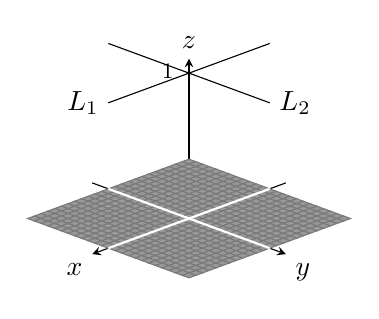
\begin{tikzpicture}
\begin{axis}[small,view/h=135,axis lines=center,colormap={}{gray(0.2cm)=(0.6);gray(1cm)=(0.9);},xlabel={$x$},ylabel={$y$},zlabel={$z$},enlargelimits=true,xtick={\empty},ytick={\empty},ztick={0,1},xlabel style={anchor={north east}},ylabel style={anchor={north west}},zlabel style={anchor={south}}]
\addplot3[surf,domain=-1:1,domain y=-1:1]{0};
\addplot3[thick,white,domain=-1:1](x,0,0);
\addplot3[thick,white,domain y=-1:1](0,y,0);
\addplot3[domain=-1:1](x,0,1)node[left]{$L_1$};
\addplot3[domain y=-1:1](0,y,1)node[right]{$L_2$};
\end{axis}
\end{tikzpicture}
\caption{تفاعل \عددی{f} چار کھلے ربعات اور لکیر \عددی{L_1}، \عددی{L_2} پر مشتمل ہے (مثال \حوالہ{مثال_کثیرالمتغیر_ٹکڑوں_میں_استمراری})۔}
\label{شکل_مثال_کثیرالمتغیر_ٹکڑوں_میں_استمراری}
\end{minipage}
\end{figure}
\جزوحصہء{استمرار اور جزوی تفرق کی موجودگی کا تعلق}
ایک نقطہ پر ایک تفاعل کا \عددی{x} اور \عددی{y} دونوں کے لحاظ سے جزوی تفرق موجود ہونے کے باوجود تفاعل غیر استمراری ہو سکتا ہے۔ یہ واحد متغیر  تفاعل سے مختلف ہے جہاں تفاعل کے تفرق کی موجودگی اس کی استمرار یقینی بناتی ہے۔ہاں (جیسا ہم اگلے حصہ میں دیکھیں گے)، اگر ایک قرص میں،  جس کا مرکز   \عددی{(x_0,y_0)} ہو،  \عددی{f(x,y)} کے جزوی تفرق موجود ہوں  جو پورے قرص میں استمراری ہوں تب \عددی{(x_0,y_0)} پر \عددی{f} استمراری ہو گا۔ 

\ابتدا{مثال}\شناخت{مثال_کثیرالمتغیر_ٹکڑوں_میں_استمراری}
درج ذیل تفاعل
\begin{align*}
f(x,y)=
\begin{cases}
0,&xy\ne 0\\
1,& xy=0
\end{cases}
\end{align*}
نقطہ \عددی{(0,0)} پر غیر استمراری ہے (شکل \حوالہ{شکل_مثال_کثیرالمتغیر_ٹکڑوں_میں_استمراری})۔ لکیر \عددی{y=x} پر چلتے ہوئے  نقطہ  \عددی{(x,y)} کا  \عددی{(x_0,y_0)} تک پہنچنے سے \عددی{f} کا حد \عددی{0} حاصل ہوتا ہے جبکہ \عددی{f(0,0)=1} ہے۔   نقطہ \عددی{(0,0)} پر \عددی{f} کے جزوی تفرقات \عددی{f_x}، \عددی{f_y}، جو شکل میں خط \عددی{L_1} اور \عددی{L_2} کی ڈھلوان ہیں،  دونوں موجود ہیں۔
\انتہا{مثال}
%===============

\جزوحصہء{دو رتبی جزوی  تفرقات}
تفاعل \عددی{f(x,y)} کو دو بار تفرق کرنے سے ہمیں  اس تفاعل کا دو رتبی تفرق ملتا ہے۔ان تفرقات کو عموماً درج ذیل سے ظاہر کیا جاتا ہے۔
\begin{align*}
\frac{\partial^{\,2}f}{\partial x^2}\quad \text{یا}\quad f_{xx}\\
\frac{\partial^{\,2}f}{\partial y^2}\quad \text{یا}\quad f_{yy}\\
\frac{\partial^{\,2}f}{\partial x \partial y}\quad \text{یا}\quad f_{yx}\\
\frac{\partial^{\,2}f}{\partial y \partial x}\quad \text{یا}\quad f_{xy}
\end{align*}
ان کی تعریفی مساوات درج ذیل ہیں
\begin{align*}
\frac{\partial^{\,2}f}{\partial x^2}=\frac{\partial}{\partial x}\big(\frac{\partial f}{\partial x}\big),\quad \frac{\partial^{\,2}f}{\partial x\partial y}=\frac{\partial}{\partial x}\big(\frac{\partial f}{\partial y}\big)
\end{align*}
جہاں تفرق لینے کی ترتیب  دھیان سے دیکھیں۔
\begin{align*}
\frac{\partial^{\,2}f}{\partial x\partial y}&=\frac{\partial}{\partial x}\big(\frac{\partial f}{\partial y}\big)&&\text{\RL{پہلے \عددی{y} اور بعد میں \عددی{x} کے ساتھ تفرق لیں}}\\
f_{yx}&=(f_y)_x&&\text{\RL{ان کا بھی یہی مطلب ہے۔}}
\end{align*}

\ابتدا{مثال}\شناخت{مثال_کثیرالمتغیر_مدغم_دو_رتبی}
اگر \عددی{f(x,y)=x\cos y+ye^x} ہو تب
\begin{align*}
\frac{\partial f}{\partial x}&=\cos y+ye^x\\
\frac{\partial^{\,2} f}{\partial y\partial x}&=\frac{\partial}{\partial y}\big(\frac{\partial f}{\partial x}\big)=-\sin y+e^x\\
\frac{\partial^{\,2} f}{\partial x^2}&=\frac{\partial}{\partial x}\big(\frac{\partial f}{\partial x}\big)=ye^x
\end{align*}
اور  درج ذیل ہوں گے۔
\begin{align*}
\frac{\partial f}{\partial y}&=-x\sin y+e^x\\
\frac{\partial^{\,2} f}{\partial x\partial y}&=\frac{\partial}{\partial x}\big(\frac{\partial f}{\partial y}\big)=-\sin y+e^x\\
\frac{\partial^{\,2} f}{\partial y^2}&=\frac{\partial}{\partial y}\big(\frac{\partial f}{\partial y}\big)=-x\cos y
\end{align*}
\انتہا{مثال}
%=================================

\جزوحصہء{مسئلہ یولر}
آپ نے مثال \حوالہ{مثال_کثیرالمتغیر_مدغم_دو_رتبی} میں دھیان دیا ہو گا کہ    مدغم      دو رتبی جزوی تفرقات
\begin{align*}
\frac{\partial^{\,2}f}{\partial y\partial x}\quad \text{}\quad \frac{\partial^{\,2}f}{\partial x\partial y}
\end{align*}
 کی قیمتیں ایک جیسی تھیں۔یہ محض اتفاق نہیں ہے۔جہاں  بھی \عددی{f}، \عددی{f_x}، \عددی{f_y}، \عددی{f_{xy}} اور \عددی{f_{yx}} استمراری ہوں یہ ایک دوسرے کے برابر ہوں گے۔

\ابتدا{مسئلہ}\شناخت{مسئلہ_کثیرالمتغیر_یولر}\موٹا{مدغم تفرق مسئلہ یا مسئلہ یولر}\\
اگر   ایک  کھلے  خطہ میں،  جس میں نقطہ \عددی{(a,b)} پایا جاتا ہو، \عددی{f(x,y)} اور اس کے جزوی تفرقات \عددی{f_x}، \عددی{f_y}، \عددی{f_{xy}} اور \عددی{f_{yx}} معین ہوں اور    \عددی{(a,b)}  پر یہ تمام  استمراری ہوں تب درج ذیل ہو گا۔
\begin{align}
f_{xy}(a,b)=f_{yx}(a,b)
\end{align} 
\انتہا{مسئلہ}
%================= 

مسئلہ یولر (مسئلہ \حوالہ{مسئلہ_کثیرالمتغیر_یولر}) کا ثبوت آپ کو  ضمیمہ \حوالہ{ضمیمہ_ط} میں ملے گا۔

مسئلہ \حوالہ{مسئلہ_کثیرالمتغیر_یولر} کہتا ہے کہ مدغم دو رتبی جزوی تفرق کے حصول میں ہم کسی بھی ترتیب سے تفرق لے سکتے ہیں۔ بعض اوقات ایسا مدد گار ثابت ہوتا ہے۔ 

\ابتدا{مثال}
درج ذیل تفاعل کے لئے \عددی{\tfrac{\partial^{\,2}w}{\partial x\partial y}} تلاش کریں۔
\begin{align*}
w=xy+\frac{e^y}{y^2+1}
\end{align*}
حل:\quad
ہمیں  \عددی{\tfrac{\partial^{\,2}w}{\partial x\partial y}} کہتا ہے کہ کہ پہلے \عددی{y} کے لحاظ سے تفرق لیں اور بعد میں \عددی{x} کے لحاظ سے تفرق لیں۔البتہ اگر ہم پہلے \عددی{x} اور بعد میں \عددی{y} کے لحاظ  سے تفرق لیں تب  نتیجہ زیادہ جلدی   اور زیادہ  آسانی سے صرف دو  قدموں  میں   حاصل ہوتا ہے۔ 
\begin{align*}
\frac{\partial w}{\partial x}&=y\\
\frac{\partial^{\,2}w}{\partial y\partial x}&=1
\end{align*}
اب  پہلے \عددی{y} اور بعد میں \عددی{x} کا تفرق لیتے ہوئے اسی کو دوبارہ حل کر کے دیکھیں۔
\انتہا{مثال}
%=================

\جزوحصہء{مزید بلند رتبہ کے جزوی تفرقات}
عملی استعمال میں یک رتبی اور دو رتبی جزوی تفرقات   زیادہ کثرت سے پائے جاتے ہیں لہٰذا ہمیں عموماً انہیں سے واسطہ ہو گا ۔جہاں تک تفاعل کے بلند تفرقات  کی بات ہے، ہم ایک تفاعل کا تفرق  جتنی بار چاہیں لیں سکتے ہیں بشرطیکہ ایسے تفرقات موجود ہوں۔ یوں ہم تین رتبی اور چار رتبی تفرقات لے سکتے ہیں جنہیں درج ذیل علامتوں  کی طرز    پر  ظاہر کیا جائے گا۔
 \begin{align*}
\frac{\partial^{\,3}f}{\partial x\partial^{\,2}y}&=f_{yyx}\\
\frac{\partial^{\,4}f}{\partial^{\,2}x\partial^{\,2}y}&=f_{yyxx}
\end{align*}
دو رتبی تفرق کی طرح،   تفرق کی ترتیب غیر اہم ہے جب تک تمام  تفرقات استمراری ہوں۔


\جزوحصہء{سوالات}
\ابتدا{سوالات}
\موٹا{یک رتبی جزوی تفرق کی تلاش}\\
سوال \حوالہ{ سوال_کثیرالمتغیر_یک_رتبی_جزوی_الف}  تا سوال  \حوالہ{سوال_کثیرالمتغیر_یک_رتبی_جزوی_ب} میں \عددی{\tfrac{\partial f}{\partial x}} اور \عددی{\tfrac{\partial f}{\partial y}} تلاش کریں۔

\ابتدا{سوال}\شناخت{ سوال_کثیرالمتغیر_یک_رتبی_جزوی_الف}
$f(x,y)=2x^2-3y-4$
\ابتدا{جواب}
\wf{\unexpanded{
$\tfrac{\partial f}{\partial x}=4x,\quad \tfrac{\partial f}{\partial y}=-3$
}}
\انتہا{جواب}
\انتہا{سوال}
%===================
\ابتدا{سوال}
$f(x,y)=x^2-xy+y^2$
\انتہا{سوال}
%====================
\ابتدا{سوال}
$f(x,y)=(x^2-1)(y+2)$
\ابتدا{جواب}
\wf{\unexpanded{
$\tfrac{\partial f}{\partial x}=2x(y+2),\quad \tfrac{\partial f}{\partial y}=x^2-1$
}}
\انتہا{جواب}
\انتہا{سوال}
%====================
\ابتدا{سوال}
$f(x,y)=5xy-7x^2-y^2+3x-6y+2$
\انتہا{سوال}
%====================
\ابتدا{سوال}
$f(x,y)=(xy-1)^2$
\ابتدا{جواب}
\wf{\unexpanded{
$\tfrac{\partial f}{\partial x}=2y(xy-1),\quad \tfrac{\partial f}{\partial y}=2x(xy-1)$
}}
\انتہا{جواب}
\انتہا{سوال}
%====================
\ابتدا{سوال}
$f(x,y)=(2x-3y)^3$
\انتہا{سوال}
%====================
\ابتدا{سوال}
$f(x,y)=\sqrt{x^2+y^2}$
\ابتدا{جواب}
\wf{\unexpanded{
$\tfrac{\partial f}{\partial x}=\tfrac{x}{\sqrt{x^2+y^2}},\quad \tfrac{\partial f}{\partial y}=\tfrac{y}{\sqrt{x^2+y^2}}$
}}
\انتہا{جواب}
\انتہا{سوال}
%====================
\ابتدا{سوال}
$f(x,y)=(x^3+y/2)^{2/3}$
\انتہا{سوال}
%====================
\ابتدا{سوال}
$f(x,y)=\frac{1}{x+y}$
\ابتدا{جواب}
\wf{\unexpanded{
$\tfrac{\partial f}{\partial x}=\tfrac{-1}{(x+y)^2},\quad \tfrac{\partial f}{\partial y}=\tfrac{-1}{(x+y)^2}$
}}
\انتہا{جواب}
\انتہا{سوال}
%====================
\ابتدا{سوال}
$f(x,y)=\frac{x}{x^2+y^2}$
\انتہا{سوال}
%====================
\ابتدا{سوال}
$f(x,y)=\frac{x+y}{xy-1}$
\ابتدا{جواب}
\wf{\unexpanded{
$\tfrac{\partial f}{\partial x}=\tfrac{-y^2-1}{(xy-1)^2},\quad \tfrac{\partial f}{\partial y}=\tfrac{-x^2-1}{(xy-1)^2}$
}}
\انتہا{جواب}
\انتہا{سوال}
%====================
\ابتدا{سوال}
$f(x,y)=\tan^{-1}\frac{y}{x}$
\انتہا{سوال}
%====================
\ابتدا{سوال}
$f(x,y)=e^{x+y+1}$
\ابتدا{جواب}
\wf{\unexpanded{
$\tfrac{\partial f}{\partial x}=e^{x+y+1},\quad \tfrac{\partial f}{\partial y}=e^{x+y+1}$
}}
\انتہا{جواب}
\انتہا{سوال}
%====================
\ابتدا{سوال}
$f(x,y)=e^{-x}\sin(x+y)$
\انتہا{سوال}
%====================
\ابتدا{سوال}
$f(x,y)=\ln(x+y)$
\ابتدا{جواب}
\wf{\unexpanded{
$\tfrac{\partial f}{\partial x}=\tfrac{1}{x+y},\quad \tfrac{\partial f}{\partial y}=\tfrac{1}{x+y}$
}}
\انتہا{جواب}
\انتہا{سوال}
%====================
\ابتدا{سوال}
$f(x,y)=e^{xy}\ln y$
\انتہا{سوال}
%====================
\ابتدا{سوال}
$f(x,y)=\sin^2(x-3y)$
\ابتدا{جواب}
\wf{\unexpanded{
$\tfrac{\partial f}{\partial x}=2\sin(x-3y)\cos(x-3y),$\\
$\tfrac{\partial f}{\partial y}=-6\sin(x-3y)\cos(x-3y)$
}}
\انتہا{جواب}
\انتہا{سوال}
%====================
\ابتدا{سوال}
$f(x,y)=\cos^2(3x-y^2)$
\انتہا{سوال}
%====================
\ابتدا{سوال}
$f(x,y)=x^y$
\ابتدا{جواب}
\wf{\unexpanded{
$\tfrac{\partial f}{\partial x}=yx^{y-1},\quad \tfrac{\partial f}{\partial y}=x^y\ln x$
}}
\انتہا{جواب}
\انتہا{سوال}
%====================
\ابتدا{سوال}
$f(x,y)=\log_y x$
\انتہا{سوال}
%====================
\ابتدا{سوال}
$f(x,y)=\int_x^yg(t)\dif t\quad \text{\RL{تمام \عددی{t} کے لئے \عددی{g} استمراری ہے}}$
\ابتدا{جواب}
\wf{\unexpanded{
$\tfrac{\partial f}{\partial x}=-g(x),\quad \tfrac{\partial f}{\partial y}=g(y)$
}}
\انتہا{جواب}
\انتہا{سوال}
%====================
\ابتدا{سوال}\شناخت{سوال_کثیرالمتغیر_یک_رتبی_جزوی_ب}
$f(x,y)=\sum\limits_{n=0}^{\infty}(xy)^n\quad (\abs{xy}<1)$
\انتہا{سوال}
%====================

سوال \حوالہ{سوال_کثیرالمتغیر_یک_رتبی_تین_متغیر_تفاعل_الف} تا سوال \حوالہ{سوال_کثیرالمتغیر_یک_رتبی_تین_متغیر_تفاعل_ب} میں \عددی{f_x}، \عددی{f_y}  اور \عددی{f_z} تلاش کریں۔

\ابتدا{سوال}\شناخت{سوال_کثیرالمتغیر_یک_رتبی_تین_متغیر_تفاعل_الف}
$f(x,y,z)=1+xy^2-2z^2$
\ابتدا{جواب}
\wf{\unexpanded{
$f_x=y^2,\quad f_y=2xy,\quad f_z=-4z$
}}
\انتہا{جواب}
\انتہا{سوال}
%===================
\ابتدا{سوال}
$f(x,y,z)=xy+yz+xz$
\انتہا{سوال}
%=====================
\ابتدا{سوال}
$f(x,y,z)=x-\sqrt{y^2+z^2}$
\ابتدا{جواب}
\wf{\unexpanded{
$f_x=1,f_y=-y(y^2+z^2)^{-1/2},$\\
$f_z=-z(y^2+z^2)^{-1/2}$
}}
\انتہا{جواب}
\انتہا{سوال}
%=====================
\ابتدا{سوال}
$f(x,y,z)=(x^2+y^2+z^2)^{-1/2}$
\انتہا{سوال}
%=====================
\ابتدا{سوال}
$f(x,y,z)=\sin^{-1}(xyz)$
\ابتدا{جواب}
\wf{\unexpanded{
$f_x=\tfrac{yz}{\sqrt{1-x^2y^2z^2}}, f_y=\tfrac{xz}{\sqrt{1-x^2y^2z^2}},$\\
$f_z=\tfrac{xy}{\sqrt{1-x^2y^2z^2}}$
}}
\انتہا{جواب}
\انتہا{سوال}
%=====================
\ابتدا{سوال}
$f(x,y,z)=\sec^{-1}(x+yz)$
\انتہا{سوال}
%=====================
\ابتدا{سوال}
$f(x,y,z)=\ln(x+2y+3z)$
\ابتدا{جواب}
\wf{\unexpanded{
$f_x=\tfrac{1}{x+2y+3z},f_y=\tfrac{2}{x+2y+3z},$\\
$f_z=\tfrac{3}{x+2y+3z}$
}}
\انتہا{جواب}
\انتہا{سوال}
%=====================
\ابتدا{سوال}
$f(x,y,z)=yz\ln(xy)$
\انتہا{سوال}
%=====================
\ابتدا{سوال}
$f(x,y,z)=e^{-(x^2+y^2+z^2)}$
\ابتدا{جواب}
\wf{\unexpanded{
$f_x=-2xe^{-(x^2+y^2+z^2)},$\\
$f_y=-2ye^{-(x^2+y^2+z^2)},$\\
$f_z=-2ze^{-(x^2+y^2+z^2)}$
}}
\انتہا{جواب}
\انتہا{سوال}
%=====================
\ابتدا{سوال}
$f(x,y,z)=e^{-xyz}$
\انتہا{سوال}
%=====================
\ابتدا{سوال}
$f(x,y,z)=\tanh(x+2y+3z)$
\ابتدا{جواب}
\wf{\unexpanded{
$f_x=\sech^2(x+2y+3z),$\\
$f_y=2\sech^2(x+2y+3z),$\\
$f_z=3\sech^2(x+2y+3z)$
}}
\انتہا{جواب}
\انتہا{سوال}
%=====================
\ابتدا{سوال}\شناخت{سوال_کثیرالمتغیر_یک_رتبی_تین_متغیر_تفاعل_ب}
$f(x,y,z)=\sinh(xy-z^2)$
\انتہا{سوال}
%=====================

سوال \حوالہ{سوال_کثیر_المتغیر_ہر_متغیر_جزوی_الف} تا سوال \حوالہ{سوال_کثیر_المتغیر_ہر_متغیر_جزوی_ب} میں ہر متغیر کے لحاظ سے تفاعل کا جزوی تفرق تلاش کریں۔

\ابتدا{سوال}\شناخت{سوال_کثیر_المتغیر_ہر_متغیر_جزوی_الف}
$f(t,\alpha)=\cos(2\pi t-\alpha)$
\ابتدا{جواب}
\wf{\unexpanded{
$\tfrac{\partial f}{\partial t}=-2\pi\sin(2\pi t-\alpha),$\\
$\tfrac{\partial f}{\partial \alpha}=\sin(2\pi t-\alpha)$
}}
\انتہا{جواب}
\انتہا{سوال}
%=================
\ابتدا{سوال}
$g(u,v)=v^2e^{2u/v}$
\انتہا{سوال}
%=================
\ابتدا{سوال}
$h(\rho,\theta,\phi)=\rho\sin\theta\cos\phi$
\ابتدا{جواب}
\wf{\unexpanded{
$\tfrac{\partial h}{\partial \rho}=\sin\theta\cos\phi,$\\
$\tfrac{\partial h}{\partial \theta}=\rho\cos\theta\cos\phi,$\\
$\frac{\partial h}{\partial \phi}=-\rho\sin\theta\sin\phi$
}}
\انتہا{جواب}
\انتہا{سوال}
%=================
\ابتدا{سوال}
$g(r,\theta,z)=r(1-\cos\theta)-z$
\انتہا{سوال}
%=================
\ابتدا{سوال}\ترچھا{قلب کا کام}\\
$W(P,H,\delta,v,g)=PH+\frac{H\delta v^2}{2g}$
\ابتدا{جواب}
\wf{\unexpanded{
$W_P(P,H,\delta,v,g)=H,$\\
$W_H(P,H,\delta,v,g)=P+\tfrac{\delta v^2}{2g},$\\
$W_{\delta}(P,H,\delta,v,g)=\tfrac{Hv^2}{2g},$\\
$W_v(P,H,\delta,v,g)=\tfrac{H\delta v}{g},$\\
$W_g(P,H,\delta,v,g)=-\tfrac{H\delta v^2}{2g^2}$
}}
\انتہا{جواب}
\انتہا{سوال}
%=================
\ابتدا{سوال}\شناخت{سوال_کثیر_المتغیر_ہر_متغیر_جزوی_ب}
$A(c,h,k,m,q)=\frac{km}{q}+cm+\frac{hq}{2}$
\انتہا{سوال}
%=================

\موٹا{دو رتبی جزوی تفرق کا حصول}\\
سوال \حوالہ{سوال_کثیرالمتغیر_تمام_جزوی_تلاش_الف} تا سوال \حوالہ{سوال_کثیرالمتغیر_تمام_جزوی_تلاش_ب} میں تفاعل کے تمام دو رتبی جزوی تفرقات تلاش کریں۔

\ابتدا{سوال}\شناخت{سوال_کثیرالمتغیر_تمام_جزوی_تلاش_الف}
$f(x,y)=x+y+xy$
\ابتدا{جواب}
\wf{\unexpanded{
$\tfrac{\partial f}{\partial x}=1+y, \tfrac{\partial f}{\partial y}=1+x,\frac{\partial^{\,2} f}{\partial x^2}=0,$\\
$\frac{\partial^{\,2} f}{\partial y^2}=0,\frac{\partial^{\,2} f}{\partial y\partial x}=\frac{\partial^{\,2} f}{\partial x\partial y}=1$
}}
\انتہا{جواب}
\انتہا{سوال}
%=================
\ابتدا{سوال}
$f(x,y)=\sin xy$
\انتہا{سوال}
%=================
\ابتدا{سوال}
$g(x,y)=x^2y+\cos y+y\sin x$
\ابتدا{جواب}
\wf{\unexpanded{
$\tfrac{\partial g}{\partial x}=2xy+y\cos x,$\\
$\tfrac{\partial g}{\partial y}=x^2-\sin y+\sin x,$\\
$\frac{\partial^{\,2} g}{\partial x^2}=2y-y\sin x,\frac{\partial^{\,2} g}{\partial y^2}=-\cos y,$\\
$\frac{\partial^{\,2} g}{\partial y\partial x}=\frac{\partial^{\,2} f}{\partial x\partial y}=2x+\cos x$
}}
\انتہا{جواب}
\انتہا{سوال}
%=================
\ابتدا{سوال}
$h(x,y)=xe^y+y+1$
\انتہا{سوال}
%=================
\ابتدا{سوال}
$r(x,y)=\ln(x,y)$
\ابتدا{جواب}
\wf{\unexpanded{
$\tfrac{\partial r}{\partial x}=\tfrac{1}{x+y},\tfrac{\partial r}{\partial y}=\tfrac{1}{x+y},\frac{\partial^{\,2} r}{\partial x^2}=\tfrac{-1}{(x+y)^2}$\\
$\frac{\partial^{\,2} r}{\partial y^2}=\tfrac{-1}{(x+y)^2},\frac{\partial^{\,2} r}{\partial y\partial x}=\frac{\partial^{\,2} f}{\partial x\partial y}=\tfrac{-1}{(x+y)^2}$
}}
\انتہا{جواب}
\انتہا{سوال}
%=================
\ابتدا{سوال}\شناخت{سوال_کثیرالمتغیر_تمام_جزوی_تلاش_ب}
$s(x,y)=\tan^{-1}\frac{y}{x}$
\انتہا{سوال}
%=================

\موٹا{مدغم جزوی تفرقات}\\
سوال \حوالہ{سوال_کثیرالمتغیر_تصدیق_مدغم_الف} تا سوال \حوالہ{سوال_کثیرالمتغیر_تصدیق_مدغم_ب}   میں \عددی{w_{xy}=w_{yx}} کی   تصدیق کریں۔

\ابتدا{سوال}\شناخت{سوال_کثیرالمتغیر_تصدیق_مدغم_الف}
$w=\ln(2x+3y)$
\ابتدا{جواب}
\wf{\unexpanded{
$\tfrac{\partial w}{\partial x}=\tfrac{2}{2x+3y},\tfrac{\partial w}{\partial y}=\tfrac{3}{2x+3y},$\\
$\frac{\partial^{\,2} w}{\partial y\partial x}=\frac{\partial^{\,2} f}{\partial x\partial y}=\tfrac{-6}{(2x+3y)^2}$
}}
\انتہا{جواب}
\انتہا{سوال}
%===============
\ابتدا{سوال}
$w=e^x+x\ln y+y\ln x$
\انتہا{سوال}
%==================
\ابتدا{سوال}
$w=xy^2+x^2y^3+x^3y^4$
\ابتدا{جواب}
\wf{\unexpanded{
$\tfrac{\partial w}{\partial x}=y^2+2xy^3+3x^2y^4,$\\
$\tfrac{\partial w}{\partial y}=2xy+3x^2y^2+4x^3y^3,$\\
$\frac{\partial^{\,2} w}{\partial y\partial x}=2y+6xy^2+12x^2y^3,$\\
$\frac{\partial^{\,2} f}{\partial x\partial y}=2y+6xy^2+12x^2y^3$
}}
\انتہا{جواب}
\انتہا{سوال}
%==================
\ابتدا{سوال}\شناخت{سوال_کثیرالمتغیر_تصدیق_مدغم_ب}
$w=x\sin y+y\sin x+xy$
\انتہا{سوال}
%==================
\ابتدا{سوال}
بغیر قلم اٹھائے   بتائیں کہ درج ذیل میں \عددی{x} کے لحاظ سے پہلے اور \عددی{y} کے  لحاظ سے بعد میں یا اس کے الٹ حل کرتے ہوئے  \عددی{f_{xy}} زیادہ جلدی حاصل ہو گا۔
\begin{enumerate}[a.]
\item
$f(x,y)=x\sin y+e^y$
\item
$f(x,y)=\frac{1}{x}$
\item
$f(x,y)=y+\frac{x}{y}$
\item
$f(x,y)=y+x^2y+4y^3-\ln(y^2+1)$
\item
$f(x,y)=x^2+5xy+\sin x+7e^x$
\item
$f(x,y)=x\ln xy$
\end{enumerate}
\ابتدا{جواب}
\wf{\unexpanded{
(ا) پہلے \عددی{x}، (ب) پہلے \عددی{y}، (ج) پہلے \عددی{x}، (د) پہلے \عددی{x}، (ہ) پہلے \عددی{y}، (ہ) پہلے \عددی{y} 
}}
\انتہا{جواب}
\انتہا{سوال}
%===============
\ابتدا{سوال}
درج ذیل میں تمام کا پانچ رتبی جزوی تفرق \عددی{\tfrac{\partial^{\,5}f}{\partial x^2\partial y^3}} صفر کے برابر ہے۔ اس کی تصدیق کرنے کی خاطر آپ کس متغیر کے لحاظ سے پہلے جزوی تفرق لیں گے؟ بغیر کچھ لکھے جواب دینے کی کوشش کریں۔
\begin{enumerate}[a.]
\item
$f(x,y)=y^2x^4e^x+2$
\item
$f(x,y)=y^2+y(\sin x-x^4)$
\item
$f(x,y)=x^2+5xy+\sin x+7e^x$
\item
$f(x,y)=xe^{y^2/2}$
\end{enumerate}
\انتہا{سوال}
%==============

\موٹا{جزوی تفرق کی تعریف کا استعمال}\\
سوال \حوالہ{سوال_کثیرالمتغیر_تعریف_حد_جزوی_تفرق_الف} اور سوال \حوالہ{سوال_کثیرالمتغیر_تعریف_حد_جزوی_تفرق_ب} میں جزوی تفرق کی تعریف بذریعہ حد استعمال کرتے ہوئے دیے گئے نقطہ پر تفاعل کا جزوی تفرق حاصل کریں۔

\ابتدا{سوال}\شناخت{سوال_کثیرالمتغیر_تعریف_حد_جزوی_تفرق_الف}
$f(x,y)=1-x+y-3x^2y,\quad \frac{\partial f}{\partial x},\,\frac{\partial f}{\partial y},\quad (1,2)$
\ابتدا{جواب}
\wf{\unexpanded{
$f_x(1,2)=-13, f_y(1,2)=-2$
}}
\انتہا{جواب}
\انتہا{سوال}
%==================
\ابتدا{سوال}\شناخت{سوال_کثیرالمتغیر_تعریف_حد_جزوی_تفرق_ب}
$f(x,y)=4+2x-3y-xy^2,\quad \frac{\partial f}{\partial x},\,\frac{\partial f}{\partial y},\quad (-2,1)$
\انتہا{سوال}
%=================
\ابتدا{سوال}
فرض کریں \عددی{w=f(x,y,z)} تین غیر تابع متغیرات کا تفاعل ہے۔ نقطہ \عددی{(x_0,y_0,z_0)} پر جزوی تفرق  \عددی{\tfrac{\partial f}{\partial z}} کی باضابطہ تعریف  لکھیں کریں۔ اس تعریف کو استعمال کرتے ہوئے \عددی{(1,2,3)} پر \عددی{f(x,y,z)=x^2yz^2} کا \عددی{\tfrac{\partial f}{\partial z}} تلاش کریں۔
\ابتدا{جواب}
\wf{\unexpanded{
$12$
}}
\انتہا{جواب}
\انتہا{سوال}
%===================
\ابتدا{سوال}
فرض کریں \عددی{w=f(x,y,z)} تین غیر تابع متغیرات کا تفاعل ہے۔ نقطہ \عددی{(x_0,y_0,z_0)} پر جزوی تفرق  \عددی{\tfrac{\partial f}{\partial y}} کی باضابطہ تعریف  لکھیں کریں۔ اس تعریف کو استعمال کرتے ہوئے \عددی{(-1,0,3)} پر \عددی{f(x,y,z)=-2xy^2+yz^2} کا \عددی{\tfrac{\partial f}{\partial z}} تلاش کریں۔
\انتہا{سوال}
%===============
\موٹا{خفی جزوی تفرقات}\\
\ابتدا{سوال}
 ذیل مساوات  میں     غیر تابع متغیرات \عددی{x} اور \عددی{y} کا تفاعل \عددی{z} پیش کیا گیا ہے۔ نقطہ \عددی{(1,1,1)} پر \عددی{\tfrac{\partial z}{\partial x}} کی قیمت تلاش کریں۔ اس نقطہ پر   یہ  جزوی تفرق  موجود ہے۔  
\begin{align*}
xy+z^3x-2yz=0
\end{align*}
\ابتدا{جواب}
\wf{\unexpanded{
$-2$
}}
\انتہا{جواب}
\انتہا{سوال}
%====================
\ابتدا{سوال}
 ذیل مساوات  میں     غیر تابع متغیرات \عددی{x} اور \عددی{y} کا تفاعل \عددی{z} پیش کیا گیا ہے۔ نقطہ \عددی{(1,-1,-3)} پر \عددی{\tfrac{\partial z}{\partial x}} کی قیمت تلاش کریں۔ اس نقطہ پر   یہ  جزوی تفرق  موجود ہے۔  
\begin{align*}
xz+y\ln x-x^2+4=0
\end{align*}
\انتہا{سوال}
%===================
سوال \حوالہ{سوال_کثیرالمتغیر_مثلث_الف} اور سوال \حوالہ{سوال_کثیرالمتغیر_مثلث_الف} درج ذیل مثلث  کے بارے میں ہے۔
\begin{center}
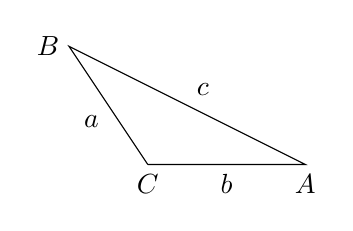
\begin{tikzpicture}
\draw(0,0)node[below]{$C$}--(2,0)node[below]{$A$}node[pos=0.5,below]{$b$}--(-1,1.5)node[left]{$B$}node[pos=0.5,above right]{$c$}--(0,0)node[pos=0.5,below left]{$a$};
\end{tikzpicture}
\end{center}

\ابتدا{سوال}\شناخت{سوال_کثیرالمتغیر_مثلث_الف}
\عددی{A} کو خفی طور پر \عددی{a}، \عددی{b} اور \عددی{c} کا تفاعل لکھ کر \عددی{\tfrac{\partial A}{\partial a}} اور \عددی{\tfrac{\partial A}{\partial b}} تلاش کریں۔
\ابتدا{جواب}
\wf{\unexpanded{
$\tfrac{\partial A}{\partial a}=\tfrac{a}{bc\sin A},\tfrac{\partial A}{\partial b}=\tfrac{c\cos A-b}{bc\sin A}$
}}
\انتہا{جواب}
\انتہا{سوال}
%=================
\ابتدا{سوال}\شناخت{سوال_کثیرالمتغیر_مثلث_ب}
\عددی{a} کو خفی طور پر \عددی{A}، \عددی{b} اور \عددی{B} کا تفاعل لکھ کر \عددی{\tfrac{\partial a}{\partial A}} اور \عددی{\tfrac{\partial a}{\partial B}} تلاش کریں۔
\انتہا{سوال}
%=================
\ابتدا{سوال}\شناخت{سوال_کثیرالمتغیر_پیچیدہ_مساوات}
غیر تابع متغیرات \عددی{x} اور \عددی{y} کی صورت میں تفاعل  \عددی{u} اور \عددی{v} مساوات \عددی{x=v\ln u} اور \عددی{y=u\ln v} دیتی ہیں۔ جزوی تفرق \عددی{v_x} ،  جو موجود ہے، کو \عددی{u} اور \عددی{v} کی صورت میں لکھیں۔ (اشارہ: دونوں مساوات کا تفرق  \عددی{x} ا کے لحاظ سے لے کر \عددی{v_x} کے لئے حل کریں۔)
\ابتدا{جواب}
\wf{\unexpanded{
$v_x=\tfrac{\ln v}{(\ln u)(\ln v)-1}$
}}
\انتہا{جواب}
\انتہا{سوال}
%=====================
\ابتدا{سوال}
غیر تابع متغیرات \عددی{u} اور \عددی{v} کی صورت میں تفاعل  \عددی{x} اور \عددی{y} مساوات \عددی{u=x^2-y^2} اور \عددی{v=x^2-y} دیتی ہیں۔ جزوی تفرق \عددی{\tfrac{\partial x}{\partial u}} اور  \عددی{\tfrac{\partial y}{\partial u}} ،  جو موجود  ہیں تلاش کریں۔ (اشارہ:سوال \حوالہ{سوال_کثیرالمتغیر_پیچیدہ_مساوات} میں دیا گیا اشارہ دیکھیں۔)   اب \عددی{s=x^2+y} لیتے ہوئے \عددی{\tfrac{\partial s}{\partial u}} حاصل کریں۔
\انتہا{سوال}
%=====================
\موٹا{مساوات لاپلاس}\\
\ترچھا{تین بعدی مساوات لاپلاس}
\begin{align}\label{مساوات_کثیر_المتغیر_مساوات_لاپلاس_الف}
\frac{\partial^{\,2}f}{\partial x^2}+\frac{\partial^{\,2}f}{\partial y^2}+\frac{\partial^{\,2}f}{\partial z^2}=0
\end{align}
کو فضا میں  برقرار حال حراری تقسیم \عددی{T=f(x,y,z)}، تجاذبی  مخفی قوہ اور برقی ساکن مخفی قوہ   مطمئن کرتے ہیں۔ مساوات \حوالہ{مساوات_کثیر_المتغیر_مساوات_لاپلاس_الف} سے جزو \عددی{\tfrac{\partial f}{\partial z}} نکالنے سے    \ترچھا{دو بعدی مساوات لاپلاس}
 \begin{align}\label{مساوات_کثیر_المتغیر_مساوات_لاپلاس_ب}
\frac{\partial^{\,2}f}{\partial x^2}+\frac{\partial^{\,2}f}{\partial y^2}=0
\end{align}
حاصل ہوتی ہے جو مستوی میں  خفی قوہ اور برقرار حال حراری تقسیم  بیان کرتی ہے۔

دکھائیں کہ سوال \حوالہ{سوال_کثیرالمتغیر_مطمئن_لاپلاس_الف} تا سوال \حوالہ{سوال_کثیرالمتغیر_مطمئن_لاپلاس_ب} میں  دیا ہر ایک  تفاعل مساوات لاپلاس میں سے کسی ایک کو مطمئن کرتا ہے۔ 

\ابتدا{سوال}\شناخت{سوال_کثیرالمتغیر_مطمئن_لاپلاس_الف}
$f(x,y,z)=x^2+y^2-2z^2$
\انتہا{سوال}
%==============
\ابتدا{سوال}
$f(x,y,z)=2z^3-3(x^2+y^2)z$
\انتہا{سوال}
%=====================
\ابتدا{سوال}
$f(x,y)=e^{-2y}\cos 2x$
\انتہا{سوال}
%=====================
\ابتدا{سوال}
$f(x,y)=\ln\sqrt{x^2+y^2}$
\انتہا{سوال}
%=====================
\ابتدا{سوال}
$f(x,y,z)=(x^2+y^2+z^2)^{-1/2}$
\انتہا{سوال}
%=====================
\ابتدا{سوال}\شناخت{سوال_کثیرالمتغیر_مطمئن_لاپلاس_ب}
$f(x,y,z)=e^{2x+4y}\cos 5z$
\انتہا{سوال}
%=====================

\موٹا{مساوات موج}\\
سمندر  کے کنارے کھڑے  ہو کر سمندری امواج کی لی گئی  تصویر  میں نشیب و فراز کا   ایک منظم نقش نظر آتا ہے۔ہمیں  فضا میں  فاصلہ کے لحاظ سے   دوری انتصابی حرکت نظر آتی ہے۔ پانی میں کھڑے ہو کر ہم گزرتی امواج کی بنا پانی کا اتار چھڑاو محسوس کرتے ہیں۔ ہم وقت کے لحاظ سے دوری انتصابی حرکت  دیکھتے ہیں۔طبیعیات  میں اس خوبصورت   تشاکلی کو \ترچھا{یک بعدی مساوات موج}
\begin{align}
\frac{\partial^{\,2}u}{\partial t^2}=c^2\frac{\partial ^{\,2}w}{\partial x^2}
\end{align}
بیان کرتی ہے جہاں  قد موج  \عددی{w}، فاصلاتی متغیر  \عددی{x}، لمحاتی متغیر \عددی{t} اور موج کی رفتار  \عددی{c}  ہے۔ 

سمندری سطح پر فاصلہ \عددی{x} ہو گا لیکن دیگر عملی استعمال میں \عددی{x}  ارتعاش پذیر  تار کے ساتھ ساتھ  فاصلہ، ہوا میں فاصلہ (صوتی امواج)، یا فضا میں فاصلہ  (امواج نور)  ہو سکتا ہے۔  عدد \عددی{c} کی قیمت موج کی قسم اور  ذریعہ پر منحصر ہو  گا۔

دکھائیں کہ سوال \حوالہ{سوال_کثیرالمتغیر_مساوات_موج_الف} تا سوال \حوالہ{سوال_کثیرالمتغیر_مساوات_موج_ب}  میں تمام  تفاعل مساوات موج کو مطمئن کرتے ہیں۔ 

\ابتدا{سوال}\شناخت{سوال_کثیرالمتغیر_مساوات_موج_الف}
$w=\sin(x+ct)$
\انتہا{سوال}
%===================
\ابتدا{سوال}
$w=\cos(2x+2ct)$
\انتہا{سوال}
%==================
\ابتدا{سوال}
$w=\sin(x+ct)+\cos(2x+2ct)$
\انتہا{سوال}
%==================
\ابتدا{سوال}
$w=\ln(2x+2ct)$
\انتہا{سوال}
%==================
\ابتدا{سوال}
$w=\tan(2x-2ct)$
\انتہا{سوال}
%==================
\ابتدا{سوال}
$w=5\cos(3x+3ct)+e^{x+ct}$
\انتہا{سوال}
%==================
\ابتدا{سوال}\شناخت{سوال_کثیرالمتغیر_مساوات_موج_ب}
\عددی{w=f(u)}؛ جہاں \عددی{f} متغیر \عددی{u} کا قابل تفرق تفاعل ،  \عددی{u=a(x+ct)} اور  \عددی{a} مستقل ہیں۔
\انتہا{سوال}
%==================

\انتہا{سوالات}

%===============================


\حصہ{تفرق  پذیری، خط بندی، اور تفرقات}
اس حصہ میں ہم تفرق پذیری کی تعریف    کے بعد  خط بندی اور تفریقیں  پیش کرتے ہیں۔ اس حصہ کے  ریاضی نتائج مسئلہ  بڑھوتری کی بنا ہیں۔ جیسا ہم اگلے حصہ میں دیکھیں گے، کثیر المتغیر تفاعل کے  زنجیری قاعدہ  کی بنیاد بھی یہی مسئلہ ہے۔

\جزوحصہء{تفرق پذیری}
تفرق پذیری کا  ابتدا نقطہ  بڑھوتری کا تصور ہے۔آپ کو یاد ہو گا کہ اگر \عددی{x=x_0} پر ایک متغیر کا تفاعل \عددی{y=f(x)} قابل تفرق ہو  تب \عددی{x} کی قیمت \عددی{x_0} سے \عددی{x_0+\Delta x}   کرنے سے \عددی{f} کی قیمت میں تبدیلی 
\begin{align}
\Delta y=f'(x_0)\Delta x+\epsilon \Delta x
\end{align}
لکھی جا سکتی ہے جہاں \عددی{\Delta x\to 0} اور \عددی{\epsilon \to 0} ہیں۔دو متغیرات کے تفاعل  کے لئے   یہی خاصیت تفرق پذیری کی تعریف  بنتی ہے۔اعلٰی  احصاء کا   مسئلہ بڑھوتری ہمیں یقین دلاتا ہے کہ یہ خاصیت  کار آمد رہے گی:

\ابتدا{مسئلہ}\شناخت{مسئلہ_کثیرالمتغیر_بڑھوتری}\موٹا{دو متغیرات کے تفاعل کا مسئلہ بڑھوتری}\\
فرض کریں    پورا کھلا  خطہ \عددی{R} میں، جس میں نقطہ \عددی{(x_0,y_0)} پایا جاتا ہو،     \عددی{f(x,y)} کے    جزوی  اول تفرقات  معین  ہیں اور \عددی{(x_0,y_0)} پر \عددی{f_x} اور \عددی{f_y} استمراری ہیں۔تب نقطہ \عددی{(x_0,y_0)} کو \عددی{R} میں    دوسری جگہ  \عددی{(x_0+\Delta x,y_0+\Delta y)} منتقل کرنے سے \عددی{f} میں رونما ہونے والی تبدیلی
\begin{align*}
\Delta z=f(x_0+\Delta x,y_0+\Delta y)-f(x_0,y_0)
\end{align*}
 درج ذیل روپ  کی مساوات کو مطمئن کرے گی جہاں \عددی{\Delta x,\, \Delta y\to 0}  کرنے سے \عددی{\epsilon_1,\,\epsilon_2\to 0} ہوں  گے۔
\begin{align}\label{مساوات_کثیرالمتغیر_تفریق_تعریف_الف}
\Delta z=f_x(x_0,y_0)\Delta x+f_y(x_0,y_0)\Delta y+\epsilon_1\Delta x+\epsilon_2\Delta y
\end{align}
\انتہا{مسئلہ}
%=================

آپ ضمیمہ \حوالہ{ضمیمہ_ط} میں  اس کا ثبوت  دیکھ کر جان سکیں گے کہ \عددی{\epsilon_1}، \عددی{\epsilon_2} کہاں سے آتے ہیں۔  آپ یہ بھی دیکھ پائیں گے کہ اسی طرح کے نتائج دو سے زیادہ  غیر تابع متغیرات کے تفاعل کے لئے کار آمد ہوں گے۔

\ابتدا{تعریف}
اگر   \عددی{f_x(x_0,y_0)} اور \عددی{f_y(x_0,y_0)}  موجود ہوں اور \عددی{(x_0,y_0)} پر \عددی{f} مساوات \حوالہ{مساوات_کثیرالمتغیر_تفریق_تعریف_الف}  کو مطمئن کرتا ہو تب \اصطلاح{\عددی{(x_0,y_0)} پر \عددی{f(x,y)} قابل تفرق}  ہو گا۔  اگر \عددی{f} اپنے دائرہ کار کے اندر ہر نقطہ پر قابل تفرق ہو تب \عددی{f}\اصطلاح{ قابل تفرق}\فرہنگ{قابل تفرق}\حاشیہب{differentiable}\فرہنگ{differentiable} ہو گا۔
\انتہا{تعریف}
%===============

اس تعریف کی روشنی میں ہمیں مسئلہ \حوالہ{مسئلہ_کثیرالمتغیر_بڑھوتری} کا  ضمنی نتیجہ ملتا ہے جس کے تحت  جس تفاعل کے   جزوی اول   تفرقات استمراری ہوں وہ تفاعل قابل تفرق ہو گا۔

\ابتدا{ضمنی نتیجہ}\موٹا{برائے مسئلہ \حوالہ{مسئلہ_کثیرالمتغیر_بڑھوتری}}
اگر پورے کھلا وقفہ \عددی{R} میں تفاعل \عددی{f(x,y)} کے جزوی تفرقات \عددی{f_x} اور \عددی{f_x} استمراری ہوں تب \عددی{R} کے ہر نقطہ پر \عددی{f} تفرق پذیر ہو گا۔
\انتہا{ضمنی نتیجہ}
%=============

  ہم مساوات \حوالہ{مساوات_کثیرالمتغیر_تفریق_تعریف_الف} میں \عددی{z} کی جگہ \عددی{f(x,y)-f(x_0,y_0)} پر کر کے اس کو
\begin{align}\label{مساوات_کثیرالمتغیر_نقطہ_پر_تفاعل_کی_قیمت}
f(x,y)=f(x_0,y_0)+f_x(x_0,y_0)\Delta x+f_y(x_0,y_0)\Delta y+\epsilon_1\Delta x+\epsilon_2\Delta y
\end{align}
لکھتے ہوئے دیکھتے ہیں کہ   اگر \عددی{\Delta x} اور \عددی{\Delta y} صفر کے قریب پہنچنے کی کوشش کرے   تب نئی مساوات کا دایاں ہاتھ \عددی{f(x_0,y_0)} کے قریب پہنچتا ہے۔اس سے ہمیں معلوم ہوتا ہے کہ تفاعل  \عددی{f(x,y)} ان تمام نقطوں پر  استمراری ہو  ہو گا جہاں یہ تفرق پذیر  ہو ۔

\ابتدا{مسئلہ}\شناخت{مسئلہ_کثیرالمتغیر_تفاعل_استمرار}
اگر نقطہ \عددی{(x_0,y_0)} پر تفاعل \عددی{f(x,y)} تفرق پذیر ہو تب \عددی{(x_0,y_0)} پر \عددی{f} استمراری ہو گا۔
\انتہا{مسئلہ}
%============

ہم مسئلہ \حوالہ{مسئلہ_کثیرالمتغیر_بڑھوتری} اور مسئلہ  \حوالہ{مسئلہ_کثیرالمتغیر_تفاعل_استمرار} سے دیکھتے ہیں کہ  اگر اس پورے  خطہ میں، جس میں  نقطہ \عددی{(x_0,y_0)} پایا جاتا ہو،     \عددی{f_x} اور \عددی{f_y} استمراری ہوں تب  \عددی{(x_0,y_0)} پر \عددی{f(x,y)} لازماً استمراری ہو گا۔  یاد رہے کہ  دو متغیرات کا تفاعل اس نقطہ پر غیر استمراری ہو سکتا ہے جہاں اس  کا جزوی اول تفرق موجود ہو (مثال \حوالہ{مثال_کثیرالمتغیر_ٹکڑوں_میں_استمراری})۔ صرف موجودگی کافی نہیں ہے۔ 

\جزوحصہء{دو متغیرات کے تفاعل کی خط بندی}
دو متغیرات کے تفاعل پیچیدہ ہو سکتے ہیں اور بعض اوقات    ہم چاہیں گے کہ  ان کی جگہ  ایسے نسبتاً  سادہ  تفاعل استعمال کریں  جن کے ساتھ کام کرنا  آسان ہو  اور جو  مخصوص عملی  استعمال میں درکار درستگی دیتے ہوں۔ہم      واحد متغیر کے تفاعل  کی خط بند ی  کی طرز پر ایسا    کرتے ہیں (حصہ \حوالہ{حصہ_استعمال_خط_بندی_اور_تفرقات})۔


فرض کریں   تفاعل \عددی{z=f(x,y)} نقطہ \عددی{(x_0,y_0)} پر  قابل تفرق ہے  اور ہم اس نقطہ پر     \عددی{f}، \عددی{f_x} اور \عددی{f_y} کی  قیمتیں  جانتے ہیں۔ ہم  اس تفاعل کا ایسا متبادل  چاہتے ہیں جو  \عددی{(x_0,y_0)}    کے قریب  موثر ہو۔ چونکہ \عددی{f} قابل تفرق ہے لہٰذا نقطہ \عددی{(x_0,y_0)} پر مساوات \حوالہ{مساوات_کثیرالمتغیر_نقطہ_پر_تفاعل_کی_قیمت}  تفاعل \عددی{f} کے لئے کار آمد ہو گا۔یوں \عددی{\Delta x=x-x_0} اور \عددی{\Delta y=y-y_0} کی بڑھوتری  سے   \عددی{(x_0,y_0)} سے نقطہ  \عددی{(x,y)}  منتقل ہونے سے \عددی{f} کی نئی قیمت
\begin{align*}
f(x,y)&=f(x_0,y_0)+f_x(x_0,y_0)(x-x_0)+f_y(x_0,y_0)(y-y_0)+\epsilon_1\Delta x+\epsilon_2\Delta y
\end{align*}
ملتی ہے جہاں \عددی{\Delta x,\Delta y\to 0} کرنے سے \عددی{\epsilon_1,\epsilon_2\to 0} ہو گا۔ اگر \عددی{\Delta x} اور \عددی{\Delta y} چھوٹے ہوں تب \عددی{\epsilon_1\Delta x} اور \عددی{\epsilon_2\Delta y} آخر کار مزید چھوٹے ہوں گے لہٰذا ہم درج ذیل لکھ سکتے ہیں۔
\begin{align*}
f(x,y)&\approx \underbrace{f(x_0,y_0)+f_x(x_0,y_0)(x-x_0)+f_y(x_0,y_0)(y-y_0)}_{L(x,y)}
\end{align*}
دوسرے لفظوں میں، جب تک \عددی{\Delta x} اور \عددی{\Delta y} چھوٹے ہوں، \عددی{f} کی قیمت تقریباً وہی ہو گی جو خطی تفاعل \عددی{L} کی ہو گی۔ اگر \عددی{f} کے ساتھ کام کرنا دشوار ہو اور \عددی{L} ہمیں درکار درستگی دیتا ہو تب ہم \عددی{f} کی جگہ \عددی{L} استعمال کر سکتے ہیں۔

\ابتدا{تعریف}
نقطہ \عددی{(x_0,y_0)}پر  ،  جہاں تفاعل \عددی{f(x,y)} قابل تفرق ہو، \عددی{f} کا\اصطلاح{  خط بند}\فرہنگ{خط بند!تفاعل}\حاشیہب{linearization}\فرہنگ{linearization} تفاعل درج ذیل ہو گا۔
\begin{align}\label{مساوات_کثیرالمتغیر_خط_بند_تخمین}
L(x,y)=f(x_0,y_0)+f_x(x_0,y_0)(x-x_0)+f_y(x_0,y_0)(y-y_0)
\end{align}
درج ذیل  تخمین
\begin{align*}
f(x,y)\approx L(x,y)
\end{align*}
  نقطہ \عددی{(x_0,y_0)} پر تفاعل \عددی{f}  کی \اصطلاح{معیاری خطی تخمین}\فرہنگ{خطی تخمین!معیاری}\حاشیہب{standard linear approximation}\فرہنگ{linear approximation!standard} ہے۔ 
\انتہا{تعریف}
%=====================

ہم دیکھیں گے کہ مستوی \عددی{z=L(x,y)} سطح \عددی{z=f(x,y)} کو  نقطہ \عددی{(x_0,y_0)} پر مماسی ہے۔یوں  جیسا واحد متغیر کی خط بندی مماسی خط تخمین دیتی ہے، اسی طرح  دو متغیرات کے تفاعل کی خط بندی ہمیں مماسی مستوی  تخمین دیتی ہے۔

\ابتدا{مثال}\شناخت{مثال_کثیرالمتغیر_خط_بند_تخمین}
نقطہ \عددی{(3,2)} پر درج ذیل کی خط بند تخمین تلاش کریں۔
\begin{align*}
f(x,y)=x^2-xy+\frac{1}{2}y^2+3
\end{align*}
حل:\quad
ہم  مساوات \حوالہ{مساوات_کثیرالمتغیر_خط_بند_تخمین} میں درج ذیل  پر کرتے ہیں۔
\begin{align*}
f(x_0,y_0)&=\big(x^2-xy+\frac{1}{2}y^2+3\big)_{(3,2)}=8\\
f_x(x_0,y_0)&=\frac{\partial}{\partial x}\big(x^2-xy+\frac{1}{2}y^2+3\big)_{(3,2)}=(2x-y)_{(3,2)}=4\\
f_y(x_0,y_0)&=\frac{\partial}{\partial y}\big(x^2-xy+\frac{1}{2}y^2+3\big)_{(3,2)}=(-x+y)_{(3,2)}=-1
\end{align*}
یوں درج ذیل حاصل ہو گا۔
\begin{align*}
L(x,y)&=f(x_0,y_0)+f_x(x_0,y_0)(x-x_0)+f_y(x_0,y_0)(y-y_0)&&\text{\RL{مساوات \حوالہ{مساوات_کثیرالمتغیر_خط_بند_تخمین}}}\\
&=8+(4)(x-3)+(-1)(y-2)=4x-y-2
\end{align*}
نقطہ \عددی{(3,2)} پر \عددی{f} کی خط بندی \عددی{L(x,y)=4x-y-2} ہے۔
\انتہا{مثال}
%================

\جزوحصہء{معیاری خطی تخمین کی درستگی}
تخمین \عددی{f(x,y)\approx L(x,y)}  میں خلل کی تلاش میں ہم \عددی{f} کے دو  رتبی  جزوی تفرقات استعمال کرتے ہیں۔ فرض کریں ایک  کھلا  سلسلہ  میں \عددی{f} کے یک رتبی اور دو رتبی جزوی تفرقات استمراری ہوں اور اس سلسلہ   میں ایک  مستطیل خطہ \عددی{R}   جس کا مرکز \عددی{(x_0,y_0)} ہو پایا جاتا ہو۔ اس مستطیل خطہ کو  درج ذیل عدم مساوات  ظاہر کرتے ہیں۔
\begin{align*}
\abs{x-x_0}\le h,\quad \abs{y-y_0}\le k
\end{align*}
چونکہ \عددی{R} بند اور محدود ہے لہٰذا \عددی{R} میں    تمام دو رتبی جزوی تفرقات  کی مطلق   زیادہ سے زیادہ قیمتیں ہوں گی۔ اگر ان میں \عددی{B} سب سے بڑی قیمت ہو تب، جیسا   آگے حصہ میں سمجھایا گیا ہے،پورے \عددی{R} میں   معیاری خطی تخمین میں خلل \عددی{E(x,y)=f(x,y)-L(x,y)}  درج ذیل عدم مساوات کو مطمئن کرے گا۔ 
\begin{align*}
\abs{E(x,y)}\le \frac{1}{2}B(\abs{x-x_0}+\abs{y-y_0})^2
\end{align*}

جب ہم اس عدم مساوات کو  \عددی{E} کی اندازاً قیمت حاصل کرنے کے لئے استعمال کریں تب ہم \عددی{f_{xx}}، \عددی{f_{yy}} اور \عددی{f_{xy}}، جو \عددی{B} تعین کرتے ہیں،  حاصل کرنے سے قاصر ہوں گے لہٰذا ہمیں  بالائی حد بندی  یعنی  بد ترین قیمت  پر گزارہ کرنا ہو گا۔   اگر   \عددی{R} میں  \عددی{\abs{f_{xx}}}، \عددی{\abs{f_{yy}}} اور \عددی{\abs{f_{xy}}}    کی مشترک بالائی حد بندی \عددی{M} ہو، تب \عددی{B} کی قیمت \عددی{M} کے برابر یا اس سے کم ہو گی لہٰذا درج ذیل ہو گا۔
\begin{align*}
\abs{E(x,y)}\le\frac{1}{2}M(\abs{x-x_0}+\abs{y-y_0})^2
\end{align*}
اس  عدم مساوات سے عموماً   \عددی{E}کی  تخمینی  قیمت حاصل کی جاتی ہے۔  کسی \عددی{M} کے لئے \عددی{\abs{E(x,y)}} کی قیمت کم کرنے کے لئے ہم \عددی{\abs{x-x_0}} اور \عددی{\abs{y-y_0}} کو چھوٹا بناتے ہیں۔

\موٹا{معیاری خطی تخمین میں خلل}\\
اگر   ایک  کھلا  سلسلہ  میں \عددی{f} کے یک رتبی اور دو رتبی جزوی تفرقات استمراری ہوں اور اس سلسلہ   میں ایک  مستطیل خطہ \عددی{R}   جس کا مرکز \عددی{(x_0,y_0)} ہو پایا جاتا ہو  اور \عددی{R} پر \عددی{\abs{f_{xx}}}، \عددی{\abs{f_{yy}}} اور \عددی{\abs{f_{xy}}}  کی بالائی حد  بندی \عددی{M} ہو   تب  \عددی{R}  پر \عددی{f(x,y)} کا متبادل 
\begin{align*}
L(x,y)=f(x_0,y_0)+f_x(x_0y_0)(x-x_0)+f_y(x_0,y_0)(y-y_0)
\end{align*}
استعمال کرنے سے پیدا خلل \عددی{E(x,y)} درج ذیل مساوات کو مطمئن کرے گا۔
\begin{align}\label{مساوات_کثیرالمتغیر_بالائی_حد_بندی_عدم_مساوات}
\abs{E(x,y)}\le \frac{1}{2}M(\abs{x-x_0}+\abs{y-y_0})^2
\end{align}


\ابتدا{مثال}
ہم نے مثال \حوالہ{مثال_کثیرالمتغیر_خط_بند_تخمین} میں \عددی{(3,2)} پر درج ذیل کی خط بندی کی۔
\begin{align*}
f(x,y)=x^2-xy+\frac{1}{2}y^2+3
\end{align*}
مستطیل 
\begin{align*}
R:\quad \abs{x-3}\le 0.1,\quad \abs{y-2}\le 0.1
\end{align*}
پر تخمین \عددی{f(x,y)\approx L(x,y)} کے خلل کی بالائی حد بندی  تلاش کریں۔اس حد بندی کو  مستطیل کے مرکز پر  \عددی{f} کی قیمت \عددی{f(3,2)} کا فی صد لکھیں۔

حل:\quad
ہم درج ذیل عدم مساوات استعمال کرتے ہیں۔
\begin{align*}
\abs{E(x,y)}&\le \frac{1}{2}M(\abs{x-x_0}+\abs{y-y_0})^2&&\text{\RL{مساوات \حوالہ{مساوات_کثیرالمتغیر_بالائی_حد_بندی_عدم_مساوات}}}
\end{align*}
ہم معمول کے تفرق سے دیکھتے ہیں کہ   \عددی{f_{xx}}، \عددی{f_{yy}} اور \عددی{f_{xy}}  تینوں مستقل  ہیں:
\begin{align*}
\abs{f_{xx}}=\abs{2}=2,\quad \abs{f_{xy}}=\abs{-1}=1,\quad \abs{f_{yy}}=\abs{1}=1
\end{align*}
ان تمام میں  سب سے بڑی قیمت   \عددی{2} ہے لہٰذا ہم \عددی{M} کو \عددی{2} کے برابر رکھ سکتے ہیں۔ اب \عددی{(x_0,y_0)=(3,2)} کے لئے \عددی{R} میں درج ذیل ہو گا۔
\begin{align*}
\abs{E(x,y)}&\le \frac{1}{2}(2)(\abs{x-3}+\abs{y-2})^2
\end{align*}
آخر میں چونکہ \عددی{\abs{x-3}\le 0.1} اور \عددی{\abs{y-2}\le 0.1} ہیں لہٰذا \عددی{R} پر 
\begin{align*}
\abs{E(x,y)}\le (0.1+0.1)^2=0.04
\end{align*}
ہو گا۔جب تب \عددی{(x,y)} مستطیل \عددی{R} میں رہے تخمین \عددی{f(x,y)\approx L(x,y)}  میں خلل \عددی{0.04} سے زیادہ نہیں ہو گی جو \عددی{R} کے مرکز پر \عددی{f} کی قیمت کا \عددی{\SI{0.5}{\percent}} ہے۔
\انتہا{مثال}
%==========

\جزوحصہء{تفریق سے تبدیلی کی پیش گوئی}
فرض  کریں ہم   نقطہ \عددی{(x_0,y_0)}   پر قابل تفرق تفاعل  \عددی{f(x,y)} اور اس کے یک رتبی تفرقات  کی قیمتیں جانتے ہیں اور ہم قریبی نقطہ \عددی{(x_0+\Delta x,y_0+\Delta y)}  پر   منتقل ہونے سے \عددی{f} کی قیمت میں تبدیلی  جاننا چاہتے  ہیں۔ اگر \عددی{\Delta x} اور \عددی{\Delta y} چھوٹے ہوں تب\عددی{(x_0,y_0)} پر  \عددی{f} اور اس کی خط بندی کی  قیمت  میں تبدیلی تقریباً ایک دوسرے جیسی ہو گی لہٰذا \عددی{L} کی تبدیلی سے ہمیں عملاً  \عددی{f} کی تبدیلی حاصل ہو گی۔

تفاعل \عددی{f}  میں تبدیلی درج ذیل ہو گی۔
\begin{align*}
\Delta f=f(x_0+\Delta x,y_0+\Delta y)-f(x_0,y_0)
\end{align*}
ہم مساوات \حوالہ{مساوات_کثیرالمتغیر_خط_بند_تخمین} میں \عددی{x-x_0=\Delta x} اور \عددی{y-y_0=\Delta y} لیتے ہوئے  \عددی{L} میں تبدیلی
\begin{align*}
\Delta L&=L(x_0+\Delta x,y_0+\delta y)-L(x_0,y_0)\\
&=f_x(x_0,y_0)\Delta x+f_y(x_0,y_0)\Delta y
\end{align*}
حاصل کرتے ہیں۔عموماً \عددی{\Delta L} کے  کلیہ  کے ساتھ کام کرنا اتنا ہی مشکل ہو گا جتنا  \عددی{\Delta f} کے کلیہ کے ساتھ کام کرنا مشکل ہو گا۔البتہ \عددی{L} میں تبدیلی \عددی{f} کے کلیہ سے حاصل کرنا زیادہ مشکل ثابت ہوتا ہے۔ خطی تخمین \عددی{L} میں تبدیلی،  ایک معلوم  مستقل ضرب \عددی{\Delta x} جمع دوسرا  معلوم  مستقل ضرب \عددی{\Delta y} ہوتا ہے۔  

ہم  تبدیلی \عددی{\Delta L} کو عموماً درج ذیل خیال آفریں  علامتی روپ    سے ظاہر کرتے ہیں جہاں\عددی{x} اور \عددی{y} میں تبدیلی \عددی{\Delta x} اور \عددی{\Delta y} کی بنا     خط بندی میں   تبدیلی کو \عددی{\dif f} ظاہر کرتی ہے۔ 
\begin{align*}
\dif f=f_x(x_0,y_0)\dif x+f_y(x_0,y_0)\dif y
\end{align*}
حسب معمول ہم \عددی{\dif x} اور \عددی{\dif y} کو \عددی{x} اور \عددی{y} کی  تفریق کہتے ہیں اور \عددی{\dif f} کو \عددی{f} کی مطابقتی  تفریق کہتے ہیں۔

\ابتدا{تعریف}
نقطہ  \عددی{(x_0,y_0)} سے قریبی نقطہ \عددی{(x_0+\Delta x,y_0+\Delta y)} منتقلی  کی بنا \عددی{f} کی  \اصطلاح{تفریق}\فرہنگ{تفریق}\حاشیہب{differential}\فرہنگ{differential} درج ذیل ہو گی۔
\begin{align}\label{مساوات_کثیرالمتغیر_کل_تفریق}
\dif f=f_x(x_0,y_0)\dif x+f_y(x_0,y_0)\dif y
\end{align}
تفاعل \عددی{f} کی خط بندی میں اس تبدیلی کو\اصطلاح{ \عددی{f} کی کل تفریق}\فرہنگ{تفریق!کل}\حاشیہب{total differential}\فرہنگ{differential!total} کہتے ہیں۔
\انتہا{تعریف}
%=================

\ابتدا{مثال}\ترچھا{تبدیلی کے لئے حساسیت }\\
آپ کا ادارہ       دائری نلکی حوض   بناتا ہے جس کا قد \عددی{\SI{25}{\meter}} اور رداس \عددی{\SI{5}{\meter}} ہے۔ قد اور رداس میں چھوٹی تبدیلی کو حوض کے حجم کی حساسیت تلاش کریں۔ 

حل:\quad
حوض کا حجم درج ذیل ہو گا۔
\begin{align*}
H(r,h)=\pi r^2 h
\end{align*}
قد اور رداس میں چھوٹی تبدیلیوں  \عددی{\dif h} اور \عددی{\dif r} کی بنا حوض کے حجم میں تبدیلی درج ذیل ہو گی۔
\begin{align*} 
\dif H&=H_r(5,25)\dif r+H_h(5,25)\dif h&&\text{\RL{مساوات \حوالہ{مساوات_کثیرالمتغیر_کل_تفریق}}}\\
&=(2\pi rh)_{(5,25)}\dif r+(\pi r^2)_{(5,25)}\dif h\\
&=250\pi\dif r+25\pi \dif h
\end{align*}
یوں \عددی{r} میں \عددی{1} اکائی تبدیلی \عددی{H} میں \عددی{250\pi} اکائیاں تبدیلی پیدا کرتی ہے جبکہ   \عددی{h} میں \عددی{1} اکائی تبدیلی \عددی{H} میں \عددی{25\pi} اکائیاں تبدیلی پیدا کرتی ہے۔ حوض کا حجم \عددی{r} میں  چھوٹی تبدیلی کو،  \عددی{h}  میں چھوٹی  تبدیلی کے لحاظ سے  \عددی{10} گنّا زیادہ حساس ہے۔ یوں آپ کو رداس پر کھڑی نظر رکھنی ہو گی۔

اس کے برعکس اگر \عددی{r} اور \عددی{h} کی قیمتیں آپس میں بدل دی جائیں تا کہ \عددی{r=\SI{25}{\meter}} اور \عددی{h=\SI{5}{\meter}} ہوں تب   کل تفریقی حجم
\begin{align*}
\dif H=(2\pi r h)_{(25,5)}\dif h+(\pi r^2)_{(25,5)}\dif r=250\pi\dif r+625\pi\dif h
\end{align*}
ہو گا۔اب حوض کا حجم قد میں تبدیلی کو زیادہ حساس ہے۔

اس مثال سے ہم یہ قاعدہ سیکھتے ہیں کہ تفاعل ان متغیرات کو زیادہ حساس ہوتے ہیں جو سب سے بڑا جزوی  تفرق دیتا ہو۔
\انتہا{مثال}
%==========

\جزوحصہء{مطلق،  نسبتی اور فی صف تبدیلی}
ایک نقطہ \عددی{(x_0,y_0)} سے قریبی نقطہ منتقلی  کی بنا تفاعل \عددی{f(x,y)}  کی قیمت میں تبدیلی کو تین مختلف طریقوں سے بیان کیا جا سکتا ہے:
\begin{center}
\renewcommand{\arraystretch}{1.5}
\begin{tabular}{RCC}
&\text{درست}&\text{اندازاً}\\
\cline{2-3}
\text{\RL{مطلق تبدیلی}}&\Delta f&\dif f\\
\text{\RL{نسبتی تبدیلی}}&\frac{\Delta f}{f(x_0,y_0)}&\frac{\dif f}{f(x_0,y_0)}\\
\text{\RL{فی صد تبدیلی}}&\frac{\Delta f}{f(x_0,y_0)}\times 100&\frac{\dif f}{f(x_0,y_0)}\times 100
\end{tabular}
\end{center}

\ابتدا{مثال}
فرض کریں متغیرات \عددی{r} اور \عددی{h} کی   قیمتوں  \عددی{(r_0,h_0)=(1,5)}  میں تبدیلی  \عددی{\dif r=0.03} اور \عددی{\dif h=-0.1} ہو۔ تفاعل \عددی{H=\pi r^2h}  کی قیمت میں مطلق، نسبتی اور فی صد تبدیلی کتنی ہو گی؟

حل:\quad
تفاعل \عددی{H} میں تبدیلی جاننے کے لئے ہم
\begin{align*}
\dif H=H_r(r_0,h_0)\dif r+H_h(r_0,h_0)\dif h
\end{align*}
کی قیمت تلاش کر کے
\begin{align*}
\dif H&=2\pi r_0h_0\dif r+\pi r_0^2h\dif h\\
&=2\pi(1)(5)(0.03)+\pi(1)^2(-0.1)=0.3\pi-0.1\pi=0.2\pi
\end{align*}
حاصل کرتے ہیں جبکہ   \عددی{H(1,5)=\pi(1)^2(5)=5\pi} ہے۔  یوں مطلق تبدیلی \عددی{0.2\pi}،  نسبتی تبدیلی \عددی{\tfrac{0.2\pi}{5\pi}=0.04} اور فی صف تبدیلی \عددی{\SI{4}{\percent}} ہو گی۔ 
\انتہا{مثال}
%==========
\ابتدا{مثال}
ایک دائری بیلن  کا حجم \عددی{H=\pi r^2h}  اس کا رداس اور قد ناپ کر حاصل کیا جاتا ہے۔ فرض کریں رداس اور قد  کی ناپ میں خلل  بالترتیب \عددی{\SI{2}{\percent}}  اور  \عددی{\SI{0.5}{\percent}} سے زیادہ نہیں ہو سکتا ہے۔حجم  کی قیمت حاصل کرنے میں خلل کتنا ہو سکتا ہے؟

حل:\quad
ہمیں درج ذیل معلومات دی گئی ہیں۔
\begin{align*}
\abs{\frac{\dif r}{r}\times 100}\le 2,\quad \abs{\frac{\dif h}{h}\times 100}\le 0.5
\end{align*}
چونکہ
\begin{align*}
\frac{\dif H}{H}=\frac{2\pi rh\dif r+\pi r^2\dif h}{\pi r^2h}=\frac{2\dif r}{r}+\frac{\dif h}{h}
\end{align*}
ہے لہٰذا 
\begin{align*}
\abs{\frac{\dif H}{H}\times 100}&=\abs{2\frac{\dif r}{r}\times 100+\frac{\dif h}{h}\times 100}\\
&\le 2\abs{\frac{\dif r}{r}\times 100}+\abs{\frac{\dif h}{h}\times 100}\le 2(2)+0.5=4.5
\end{align*}
ہو گا۔ہمارا اندازہ  ہے کہ حجم  کے حساب میں خلل  \عددی{\SI{4.5}{\percent}} سے زیادہ نہیں ہو گا۔
\انتہا{مثال}
%================

ہمیں \عددی{r} اور \عددی{h} کتنی درستگی سے ناپنا ہو گا تا کہ حجم کے حساب میں خلل  مثلاً \عددی{\SI{2}{\percent}} سے زیادہ نہ ہو؟ اس طرح کے سوالات کا جواب دینا مشکل ہے چونکہ اس کا کوئی ایک صحیح جواب نہیں پایا جاتا ہے۔چونکہ
\begin{align*}
\frac{\dif H}{H}=2\frac{\dif r}{r}+\frac{\dif h}{h}
\end{align*}
ہے لہٰذا \عددی{\tfrac{\dif H}{H}} کو \عددی{\tfrac{\dif r}{r}} اور \عددی{\tfrac{\dif h}{h}}  مل کر قابو کرتے ہیں۔اگر ہم \عددی{h} درست  ناپ سکیں تب  عین  ممکن ہے کہ \عددی{r} کی ناپ زیادہ درست نہ ہونے کی صورت میں بھی ہمیں درکار نتائج  ملیں۔ اس کے برعکس    \عددی{h} کی ناپ اتنی ناقص ہو سکتی ہے کہ ہم جتنا چاہیں \عددی{r} کی ناپ درست رکھیں، نتائج قابل قبول نہ ہوں۔

ایسی صورت میں ہم ناپی گئی قیمتوں  \عددی{(r_0,h_0)}  کو مرکز رکھتے ہوئے ایک مربع  منتخب کرتے ہیں جس میں \عددی{H} کی  قیمت \عددی{\pi r_0^2h_0} سے قابل قبول حد سے زیادہ تجاوز نہ کرتا ہو۔
%=================
\ابتدا{مثال}
نقطہ \عددی{(r_0,h_0=(5,12)} کو مرکز رکھتے ہوئے ایسا مربع تلاش کریں جس میں حجم \عددی{H=\pi r^2h} کی   قیمت \عددی{\pm 0.1} سے زیادہ تجاوز نہ کرے۔

حل:\quad
ہم \عددی{\dif H} کی درج ذیل تخمین  لیتے ہیں۔
\begin{align*}
\dif H=2\pi r_0h_0\dif r+\pi r_0^2\dif h=2\pi(5)(12)\dif r+\pi(5)^2\dif h=120\pi\dif r+25\pi\dif h
\end{align*}
چونکہ ہم جس خطہ کے اندر رہنا چاہتے ہیں وہ خطہ ایک  مربع  ہے لہٰذا ہم \عددی{\dif h=\dif r} لے  کر
\begin{align*}
\dif H=120\pi \dif r+25\pi\dif r=145\pi\dif r
\end{align*}
حاصل کرتے ہیں۔ ہم اب پوچتھے  ہیں، \عددی{\dif r} کتنا چھوٹا ہونا چاہیے تا کہ \عددی{\abs{\dif H}} ی قیمت \عددی{0.1} سے کسی صورت زیادہ نہ ہو؟ ہم عدم مساوات
\begin{align*}
\abs{\dif H}\le 0.1
\end{align*}
سے شروع کر کے \عددی{\dif H} کو \عددی{\dif r} کی صورت 
\begin{align*}
\abs{145\pi\dif r}\le 0.1
\end{align*}
میں لکھ کر \عددی{\dif r} کی بالائی حد بندی تلاش کرتے ہیں:
\begin{align*}
\abs{\dif r}\le \frac{0.1}{145\pi}&\approx 2.1\times 10^{-4}&&\text{\RL{نیچے  پورا کرتے ہیں تا کہ غلطی سے \عددی{\dif r} بڑا نہ ہو جائے}}
\end{align*}
اب \عددی{\dif h=\dif r} کی بنا ہمارا مربع درج ذیل مساوات دیں گے۔
\begin{align*}
\abs{r-5}\le 2.1\times 10^{-4},\quad \abs{h-12}\le 2.1\times 10^{-4}
\end{align*}
جب تک \عددی{(r,h)} اس مربع میں رہیں، ہم توقع کر سکتے ہیں کہ \عددی{\abs{\dif H}} کی قیمت \عددی{0.1} کے برابر یا اس سے کم ہو گی اور ہم توقع کر سکتے ہیں کہ \عددی{\abs{\Delta H}}  بھی تقریباً اتنا ہو گا۔
\انتہا{مثال}
%=====================
\جزوحصہء{دو سے زیادہ متغیرات کے تفاعل}
دو سے زیادہ متغیرات کے تفاعل کے لئے بھی ایسا ہو گا۔
\begin{enumerate}[1.]
\item
نقطہ \عددی{N_0(x_0,y_0,z_0)} پر تفاعل \عددی{f(x,y,z)} کی خط بندی  درج ذیل ہو گی۔
{\small{
\begin{align}\label{مساوات_کثیرالمتغیر_تین_متغیر_تفاعل_تخمین}
L(x,y,z)=f(N_0)+f_x(N_0)(x-x_0)+f_y(N_0)(y-y_0)+f_z(N_0)(z-z_0)
\end{align}
}}
\item
فرض کریں بند  ٹھوس مستطیل  \عددی{R} کا مرکز \عددی{N_0} ہے۔ یہ مستطیل ایسے خطہ میں پایا جاتا ہے جہاں \عددی{f} کے دو رتبی جزوی تفرقات استمراری ہیں۔ مزید فرض کریں کہ پورے \عددی{R} پر \عددی{\abs{f_{xx}}}،  \عددی{\abs{f_{yy}}}،  \عددی{\abs{f_{zz}}}،  \عددی{\abs{f_{xy}}}،  \عددی{\abs{f_{xz}}} اور  \عددی{\abs{f_{yz}}} کی قیمتیں \عددی{M} کے برابر یا اس سے کم ہیں۔تب پورے \عددی{R} میں   \عددی{f} کی تخمین \عددی{L} میں \اصطلاح{خلل}\فرہنگ{خلل}\حاشیہب{error}\فرہنگ{error} \عددی{ٰE(x,y,z)=f(x,y,z)-L(x,y,z)}کی بالائی حد بندی   درج ذیل عدم مساوات دے گی۔
\begin{align}\label{مساوات_کثیرالمتغیر_تین_متغیر_تفاعل_خلل}
\abs{E}\le \frac{1}{2}M(\abs{x-x_0}+\abs{y-y_0}+\abs{z-z_0})^2
\end{align} 
\item
اگر \عددی{f} کے  دو رتبی جزوی تفرقات استمراری ہوں اور \عددی{x}، \عددی{y}، \عددی{z} کی قیمتیں  چھوٹی تبدیلیوں \عددی{\dif x}، \عددی{\dif y}، \عددی{\dif z} کی بنا  \عددی{x_0}، \عددی{y_0}، \عددی{z_0} سے تبدیل ہو جائیں ، تب کل  تفریق
\begin{align*}
\dif =f_x(N_0)\dif x+f_y(N_0)\dif y+f_z(N_0)\dif z
\end{align*}
تفاعل \عددی{f} میں نتیجتاً تبدیلی کی اچھی تخمین ہو گی۔
\end{enumerate}

\ابتدا{مثال}
نقطہ \عددی{(x_0,y_0,z_0)=(2,1,0)} پر درج ذیل تفاعل کی خط بندی \عددی{L(x,y,z)} تلاش کریں۔
\begin{align*}
f(x,y,z)=x^2-xy+3\sin z
\end{align*}
تفاعل \عددی{f} کی جگہ تخمین \عددی{L} استعمال کرنے سے درج ذیل مستطیل میں   پیدا خلل کی بالائی حد بندی دریافت کریں۔
\begin{align*}
R:\quad \abs{x-2}\le 0.01,\quad \abs{y-1}\le 0.02,\quad \abs{z}\le 0.01
\end{align*}
حل:\quad
ہم پلہے درج ذیل معلوم کرتے ہیں۔
\begin{align*}
f(2,1,0)=2, f_x(2,1,0)=3, f_y(2,1,0)=-2,f_z(2,1,0)=3
\end{align*}
ان قیمتوں کو استعمال کرتے ہوئے  مساوات \حوالہ{مساوات_کثیرالمتغیر_تین_متغیر_تفاعل_تخمین} درج ذیل دیتی ہے۔
\begin{align*}
L(x,y,z)=2+3(x-2)+(-2)(y-1)+3(z-0)=3x-2y+3z-2
\end{align*}
اسی طرح پہلے دو رتبی جزوی تفرقات حاصل کرتے ہیں۔
\begin{align*}
f_{xx}=2, f_{yy}=0, f_{zz}=-3\sin z, f_{xy}=-1,f_{xz}=0,f_{yz}=0
\end{align*}
مساوات \حوالہ{مساوات_کثیرالمتغیر_تین_متغیر_تفاعل_خلل} میں \عددی{M} کو \عددی{\abs{-3\sin z}} کی زیادہ سے زیادہ قیمت یعنی \عددی{3} لے سکتے ہیں۔یوں 
\begin{align*}
\abs{E}\le \frac{1}{2}(3)(0.01+0.02+0.01)^2=0.0024
\end{align*}
ہو گا لہٰذا خلل \عددی{0.0024} سے زیادہ نہیں ہو گا۔
\انتہا{مثال}
%===========
\ابتدا{مثال}\ترچھا{یکساں بار بردار شہتیر کی جھول }\\
ایک افقی مستطیل شہتیر جس کے  دونوں سروں کو  سہارا دیا گیا  اور جس پر یکساں بوجھ (یکساں وزن فی میٹر لمبائی) ڈالا گیا ہو  اس  بوجھ کے نیچے جھک جائے گا۔ جھکاو \عددی{S}  کو درج ذیل کلیہ سے معلوم کیا جا سکتا ہے ۔
\begin{align*}
S=C\frac{px^4}{wh}
\end{align*}
اس مساوات میں متغیرات کی تفصیل درج ذیل ہے۔
\begin{description}
\item{p}\quad
بوجھ (شہتیر کے ایک میٹر پر وزن ۔وزن کی اکائی نیوٹن ہے۔)
\item{x}\quad
دونوں سروں پر سہارا کے بیچ فاصلہ (میٹر)
\item{w}\quad
شہتیر کی چوڑائی (میٹر)
\item{h}\quad
شہتیر کا قد (میٹر)
\item{C}\quad
ایک مستقل  جو اس مادہ پر منحصر ہو گا جس سے شہتیر بنایا گیا ہو۔
\end{description}
ایک شہتیر کی   لمبائی \عددی{\SI{4}{\meter}}، چوڑائی  \عددی{\SI{10}{\centi\meter}}  اور   قد  \عددی{\SI{20}{\centi\meter}}  ہیں۔اس پر \عددی{\SI{100}{\newton\per\meter}} بوجھ ڈالا گیا ہے۔ جھول میں تبدیلی  \عددی{\dif S}  سے شہتیر کے بارے میں کیا نتیجہ حاصل کیا جا سکتا ہے؟

حل:\quad
چونکہ \عددی{S} چار متغیرات \عددی{p}، \عددی{x}، \عددی{w}، \عددی{h} کا تفاعل ہے لہٰذا اس  کی  کل تفریق \عددی{\dif S} درج ذیل ہو گی۔
\begin{align*}
\dif S=S_p\dif p+S_x\dif x+S_w\dif w+S_h\dif h
\end{align*}
کسی مخصوص \عددی{p_0}، \عددی{x_0}، \عددی{w_0}، \عددی{h_0} کے لئے اس کو حل کرتے ہوئے  مساوات کی سادہ صورت حاصل کرنے سے  
\begin{align*}
\dif S=S_0\big(\frac{\dif p}{p_0}+\frac{4\dif x}{x_0}-\frac{\dif w}{w_0}-\frac{3\dif h}{h_0}\big)
\end{align*}
ملتا ہے جہاں \عددی{S_0=S(p_0,x_0,w_0,h_0)=Cp_0x_0^4/(w_0h_0^3)} ہے۔

اگر \عددی{p_0=\SI{100}{\newton\per\meter}}، \عددی{x_0=\SI{4}{\meter}}، \عددی{w_0=\SI{0.1}{\meter}} اور \عددی{h_0=\SI{0.2}{\meter}} ہوں تب
\begin{align}
\dif S=S_0\big(\frac{\dif p}{100}+\dif x-10\dif w-15\dif h\big)
\end{align}
اس مساوات میں چونکہ \عددی{\dif p} اور \عددی{\dif x} کے عددی سر  مثبت ہیں لہٰذا \عددی{p} اور \عددی{x} جھول بڑھاتے ہیں۔ اس کے برعکس \عددی{\dif w} اور \عددی{\dif h} کے عددی سر  منفی ہیں لہٰذا \عددی{w} اور \عددی{h} جھول کم کرتے ہیں۔ چونکہ \عددی{\dif p} کا عددی سر \عددی{\tfrac{1}{100}} ہے لہٰذا بوجھ کا جھول پر زیادہ اثر نہیں ہو گا۔ چونکہ \عددی{\dif h} کا عددی سر \عددی{\dif w} کے عدی سر سے بڑا ہے لہٰذا  شہتیر کا قد \عددی{\SI{1}{\centi\meter}} بڑھانے سے جھول زیادہ کم ہو گا۔
\انتہا{مثال}
%========================
